\documentclass[12pt]{article}
\usepackage[utf8]{inputenc}
\usepackage{fancyhdr}
\usepackage{xspace}
\usepackage{systeme}
\usepackage{authblk}
\usepackage{hyperref}



\usepackage{TFG}
\linespread{1.5}
%\pagestyle{fancy}
%\rhead{}
%\lhead{}
\date{}

\renewcommand\Authfont{\fontsize{12}{14.4}\selectfont}
\renewcommand\Affilfont{\fontsize{9}{10.8}\itshape}

\title{Stochastic Parametrisations Using Operator Expansions}

\author[1,2]{Manuel Santos Gutiérrez}
\author[1,2,3]{Valerio Lucarini}
\affil[1]{Department of Mathematics and Statistics, University of Reading, Reading, U.K.}
\affil[2]{Centre for the Mathematics of Planet Earth, University of Reading, Reading, U.K.}
\affil[3]{CEN-Meteorological Institute, University of Hamburg, Hamburg, Germany}

\begin{document}
\maketitle

\begin{abstract}
We use formal perturbative expansions of the Koopman operator to derive stochastic parametrisations of weakly coupled dynamical systems. Such parametrisation yields a set of stochastic integro-differential equations with explicit noise and memory kernel formulae, describing the effects of unresolved variables. In this document, we clarify that the perturbation expansions need not be truncated when the coupling is additive and state some conditions for when such integro-differential equation can be recast to a simpler Markovian model. Finally, we compare this methodology with well-establish data-driven protocols which have been proven to provide rigorous dynamical closures to partially observed systems. The general aim is to provide a conceptual basis for the link between empirical and theoretical approaches to stochastic paramatrisation.
\end{abstract}
\section{Introduction}

 Obtaining useful parametrisations of models is a central problem in science, especially in the context of geophysics. Parametrisations aim at creating reduced order models that are able to capture the main dynamical and statistical properties of the complete ones. A primary example of the usefulness of parametrisations is in numerical weather prediction, where microphysical processes (like cloud physics) are parametrised and incorporated into the evolution equation for the prognostic variables. The procedures in this matter not only differ on their implementation and level of accuracy, but also in their conceptual basis.

Given a high-dimensional dynamical system, we are interested in rewriting it where only the variables of interest are resolved. A first-guess would be to ignore the unresolved variables and consider uniquely the evolution laws for target process. However, this is well-known to be insuficient. A step forward, would be to consider canonical projections onto the set of resolved variables, although this incurs non-trivial modifications to the dynamics. Indeed, by working at the level of observables, Mori and Zwanzig \cite{zwanzig} clarifyied that the evolution laws for the projected dynamics necessarily incorporate explicitly the instant and delayed effects of the hidden processes. Formally, let $\Phi$ denote a generic observable defined on $\mathcal{X}\times \mathcal{Y}$ and let us define $\mathbb{P}$ as a canonical projection onto the set of target variables $\mathcal{X}$. The complementary projection we denote as $\mathbb{Q}=1 - \mathbb{P}$. Moreover, the instantaneous change with respect to time of $\Phi$ is governed by the linear operator $\LLL$, whose exponential maps the values of $\Phi$ at time $0$ to those at a prescribed time $t$: $\Phi(\xx, \yy , t)=e^{t\LLL}\Phi(\xx,\yy)$. The operator defined this way is the Koopman operator and the family of Koopam operators indexed in time form a semigroup (more details are provided later in the text).  Then, its time evolution satisfies the following chain of equalities:
\begin{align}
\partial _t \Phi(\xx,\yy , t) &= \mathcal{L} \Phi(\xx,\yy , t) = \mathcal{L} e^{t\LLL}\Phi(\xx,\yy)= e^{t\LLL}\mathcal{L}\Phi(\xx,\yy)= e^{t\LLL}\left(\mathbb{P}+\mathbb{Q}\right)\mathcal{L}\Phi(\xx,\yy) \\ \label{mori zwanzig 2} &= e^{t\LLL}\mathbb{P}\LLL\Phi(\xx,\yy) + e^{t\mathbb{Q}\LLL}\mathbb{Q}\LLL\Phi(\xx,\yy) + \int_{0}^{t}e^{(t-s)\LLL}\mathbb{P}\LLL e^{s\mathbb{Q}\LLL}\mathbb{P}\mathbb{Q}\LLL \Phi(\xx,\yy) \dd s
\end{align}
where we have emplyed the Dyson identity \cite{engelsemigroups2006}, that will be revisited later in the text. The first term in Eq.~(\ref{mori zwanzig 2}) indicates the evolution due to the resolved variables alone. The second models the fluctuating effects due to the evolution of the  $\yy$-variables. Lastly, there is an integral component that takes into account a delayed influence of the unresolved variables in $\mathcal{Y}$. This formal calculation suggests that any model for the $\xx$-variables should incorporate a fluctuating and a memory or integral term. Unfortunately, this Mori-Zwanzig equation is implicit since it does not give formulae for each of the components. Hence, we say that a parametrisation is an explicit candidate susceptible of approximating the Mori-Zwanzig equation.

The objective of this report is to study the weak-couping limit (WL) parametrisation presented in \cite{Wouters2012, wouters2013} and investigate how the Dyson expansions can be used to derive explicit formulae for the fluctuating and memory corrections suggested by the Mori-Zwanzig calculation. Here we shall clarify that the Dyson expansions need not be truncated for addtively coupled models and consider more general coupling laws than those in \cite{wouters2013}. Moreover, we revisit the problem of finding Markovian representations of the memory equation yielded by the WL approach.

Data-driven protocols also provide candidates for the Mori-Zwanzig memory equation. Indeed, partial observations of a time-evolving system can be used to deduce the fluctuating and delayed effects of the unobserved processes. This is attained by using Empirical Model Reduction (EMR) approaches that have been analysed in a geophyiscal context \cite{Kravtsov2005} and shown to provide optimal dynamical closures \cite{kondrashovdata2015}. The multilevel structure of these models (Multilevel Stochastic Models) allows for establishing dynamical properties that can ultimately provide explicit formulae for the fluctuating and memory corrections that parametrise the influence of hidden processes.

The aforementioned methodologies are conceptually and practically different, even if the ultimate target is to provide a candidate for the Mori-Zwanzig integro-differential equation. In other words, they both provide fluctuations in the form of stochastic noise and memory effects determined by an integral kernel. On the one hand, the WL approach assumes prior knowlege about the (decoupled) hidden dynamics but no information about the statistical properties of the coupled system. The empirical approach, on the other hand, samples the observed variables evolving according to the coupled regime. In this sense one can refer to these methodologies as \emph{top-down} or \emph{bottom-up}. This distinction is illustrated in Figure \ref{schematic}, where, starting from the top box, one can arrive at a memory equation (like in the Mori-Zwanzig calculation) via \emph{top-down} or \emph{bottom-up} methods indicated by the left and right branches respectively. Hence, the general goal is to provide a conceptual link between these two approaches by explaining the arrows in such figure.

The document is structured as follows. The second section is devoted to applying the Dyson expansion to the Koopman operator associated with two weakly coupled dynamical systems. We eventually derive the WL parametrisation and discuss the possibility of recasting it into a Markovian system. The third section revisits the concept of Multilevel Stochastic Models and its connection with the EMR. In the Results section, we apply the two discussed methodologies into a conceptual stochastic climate model. Finally, we discuss the conclusions obtained from this investigation.

\begin{figure}[H]
	\centering
	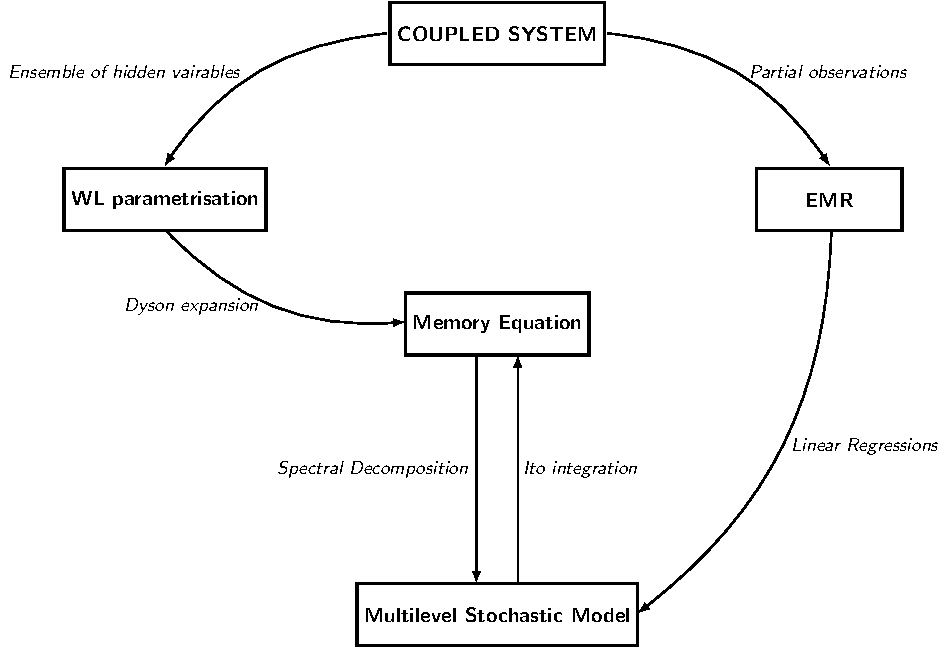
\includegraphics[width=\textwidth]{plots/general/scheme_parametrisation.pdf}
	\caption{\label{schematic}Schematic view of the different methodologies studied in this document. The arrows on the left-hand side indicate top-down parametrisations; on the right, refer to bottom-up/empirical procedures.}
\end{figure}

\section{Weak-Coupling Limit Parametrisation}\label{weak-coupling limit parametrisation}

An example of the application of stochastic parametrisations is the study of coupled models describing different phenomena. In the limit of weak coupling one realises that the coupling can be treated as a perturbation to the main dynamics, regardless of the time-scale separation \cite{Wouters2012, wouters2013, lucariniwouters}. This is particularly relevan in climate physics, where there is not clear time-scale separation at hand. Under such assumption and some degree of structual stability of the dynamics, reponse theory can be applied to derive explicit stochastic and memory terms in the spirit of the Mori-Zwanzig formalism. Here, we shall revise the derivation of the parametrisation presented in \cite{wouters2013, lucariniwouters}, using perturbative expansions of the Koopman operator.

Formally, we want to couple two dynamical systems generated independently by two vector fields $\FFF : \mathcal{X}\subseteq \mathbb{R}^{d_1} \longrightarrow \mathcal{X}$ and $\GGG : \mathcal{Y}\subseteq \mathbb{R}^{d_2}\longrightarrow \mathcal{Y}$ of, possibly, different dimensions $d_1,d_2\in \mathbb{N}$. Then, by imposing some coupling law between the systems, we consider an extended version of the form:
\begin{align}
	\label{mle1}
	\dot{\mathbf{x}}(t) &= \FFF(\mathbf{x}(t)) + \epsilon \CCC_{\xx}^{\xx}\left(\xx(t) \right) : \CCC_{\yy}^{\xx}\left(\yy(t) \right) \\
	\label{mle2}
	\dot{\mathbf{y}}(t) &= \GGG(\mathbf{y}(t)) + \epsilon \CCC_{\xx}^{\yy}\left(\xx(t) \right):\CCC_{\yy}^{\yy}\left(\yy(t) \right)
\end{align}
where new vector fields have been introduced to model such coupling law:
	$\CCC_{\xx}^{\xx}:\mathcal{X} \longrightarrow \mathcal{X}$, $\CCC_{\xx}^{\yy}: \mathcal{Y} \longrightarrow \mathcal{X}$, $\CCC_{\yy}^{\xx}:\mathcal{X} \longrightarrow \mathcal{Y}$ and $\CCC_{\yy}^{\yy}:\mathcal{Y} \longrightarrow \mathcal{Y}$. The parameter $\epsilon \in \mathbb{R}$ represents the strength of the coupling between the two processes. It is clear, then, that the uncoupled scenario is attained at $\epsilon = 0$. The product indicated by $:$ denotes pointwise multiplication between the components of a vector. The reason for doing this is that we will require that each component of the coupling vector fields is separable in $\xx$ and $\yy$. 
	

The novelty introduced in the WL parametrisation is that the coupling is viewed as an $\epsilon$-perturbation of the otherwise independent processes $\xx$ and $\yy$. Using this viewpoint and assuming structural stability of the $\xx$-process, response formulas can be used to derive an effective equation for the $\xx$-variables which are assumed to be (with no loss of generality) slow or observed, whereas the motion of $\yy$ is hidden and its manifestation is only implicit via its effects on the observed motion. Furthermore, by performing operator expansions of the Mori-Zwanzig equation in terms of the coupling parameter, one realises that the fluctuation and memory terms predicted using response-theoretic approaches match to second order in $\epsilon$.

Taking the point of view of Mori and Zwanzig, we wish to calculate the evolution of observables that only depend on the observed variables $\xx$. The idea, following \cite{wouters2013}, is to perform perturbative expansions on the operators governing the evolution of observables, as will be explained in the lines below. In general, a generic $\mathcal{C}^{\infty}$-observable $\Phi : \mathcal{X}\times \mathcal{Y} \longrightarrow \mathbb{R}$ evolves according to the Liouville equation:
\begin{equation}\label{liouville equation}
	\partial _t \Phi \left( \xx , \yy , t \right) = \LLL (\xx ,\yy)\Phi \left( \xx , \yy , t \right),
\end{equation}
where we have introduced the operator $\LLL\left(\xx , \yy\right) : \CC ^{\infty}\left( \mathcal{X}\times \mathcal{Y} \right)\longrightarrow \CC ^{\infty}\left( \mathcal{X}\times \mathcal{Y} \right)$ for every $(\xx , \yy)\in \mathcal{X}\times \mathcal{Y}$. This operator, dropping the $(\xx,\yy)$-dependence, can be splittled into $\LLL = \LLL_0 +\epsilon \LLL_1$, where $\LLL_1$ accounts for the component of the equation arising when $\epsilon \neq 0$, conversely we define $\LLL_0$. More specifically,
\begin{align}
	\LLL_0 &= \begin{bmatrix}
	\FFF (\xx) \\ \GGG (\yy)
	\end{bmatrix}\cdot \begin{bmatrix}
	\partial_{\xx} \\ \partial_{\yy}
	\end{bmatrix}\Phi (\xx, \yy , t), \\
		\epsilon \LLL_1 &= \epsilon \begin{bmatrix}
	 \CCC_{\xx}^{\xx}\left(\xx \right) : \CCC_{\yy}^{\xx}\left(\yy \right) \\ \CCC_{\xx}^{\xx}\left(\xx \right) : \CCC_{\yy}^{\xx}\left(\yy \right)
	\end{bmatrix}\cdot \begin{bmatrix}
	\partial_{\xx} \\ \partial_{\yy}
	\end{bmatrix} \Phi (\xx, \yy , t).
\end{align}
It is, therefore, clear that the operators are differential linear operators. The solution operator of Eq.~(\ref{liouville equation}) is sometimes referred to as the Koopman operator which descibes how functions of phase-space change under the action of the flow. Its dual acts on densities and it is the so-called \emph{transfer operator}. This equation is a transport equation, where the physical quantity or observable $\Phi$ is advected according to the vector field given in Eq.~(\ref{mle1}) and (\ref{mle2}). So far, the exposition has been done in the context of deterministic dynamical systems, however, one of the advantages of using the linear operator formalism is that these equations can be analogously formulated for Markov difussion processes driven by stochastic forcing. In this case, the Koopman operator turns into the so-called \emph{backward-Kolmogorov} equation describing, instead, the evolution of the expected value of observables. This, loosely speaking, amounts to adding a Laplacian operator to the operator $\LLL$. 

The solution of the Liouville equation constitutes a family of linear operators indexed in time $\{T^t\}_{t\in \mathbb{R}}$ that are, formally, defined as the exponential of the operator $\LLL$, i.e., $T^t=e^{t\LLL}$. This family has the structure of a strongly continuous contracting semigroup and has a very explicit definition:
\begin{equation}
T^t\Phi(\xx, \yy , t) = e^{t\LLL}\Phi (\xx , \yy ,t ) = \Phi (\xx(t),\yy(t)),
\end{equation}
where $(\xx(t),\yy(t))$ is a solution at time $t$ of the original system for a given initial condition. This semigroup is known as the Koopman semigroup and for each $t$, $T^t$ is referred to as the Koopman operator. The nature of the spectrum of these operators can given insight to the statistical properties of the system, although we shall not delve into this problem as it is out of the scope of the present manuscript. If the coupling parameter $\epsilon$ is small, one can use perturbation expansions of the Koopman semigroup so that one can isolate the effects of introducing the coupling at the level of observables. The perturbation expansion we do here was first introduced in the context of quantum electrodynamics \cite{Dyson1949} and later formulated rigorously in mathematical terms. Formally, we have that:
\begin{align} 
\Phi(\xx(t),\yy(t)) &= e^{t\LLL}\Phi(\xx,\yy)=e^{t\LLL_0+t\epsilon \LLL_1}	\Phi(\xx,\yy) \\\label{pertexp1} &= e^{t\LLL_0}\Phi(\xx,\yy)+\epsilon\int_{0}^te^{s\LLL}\LLL_1e^{(t-s)\LLL_0}\Phi(\xx,\yy)\dd s\\\label{pertexp2}  &= e^{t\LLL_0}\Phi(\xx,\yy)+\epsilon\int_{0}^te^{(t-s)\LLL_0}\LLL_1e^{s\LLL}\Phi(\xx,\yy)\dd s \\\label{pertexp3}&= e^{t\LLL_0}\Phi(\xx,\yy)+\epsilon\int_{0}^te^{(t-s)\LLL_0}\LLL_1e^{s\LLL_0}\Phi(\xx,\yy)\dd s + \mathcal{O}\left(\epsilon^2\right).
\end{align}
These identities show that the evolution of the value of a generic observable can be described as a perturbation to its evolution in the decoupled regime. We note that these expressions are purely formal. It is not made clear in which sense this expansion converges. In the case of the pertuabtion operator $\LLL_1$ being a bounded operator, it would be straightforward to proof boundedness of the resulting perturbed semigroup. However, the operator we are dealing with here is a differential linear operator, for which direct estimates of the integrals above cannot be taken. Nevertherless we shall stick to this formulation thorughout the text.

The aim now is to use these operator techniques to derive an effective parametrised equation for the evolution of the $\xx$-variables without explicitly solving the $\yy$-process. We desire to start observing the system at $t=0$, but assuming that the system has already attained a steady state. Since we are only concerned with observables depending on the $\xx$-variables, we shall formulate an evolution equation for them. For that we consider the Liouville equation for a generic $\yy$-independent observable $\Phi$. Then, at the time we start observing the coupled system, we have:
\begin{equation}\label{init liouville}
	\partial _t \Phi \left( \xx , \yy , t \right)|_{t=0} = \left[ \FFF(\xx) + \epsilon \CCC_{\xx}^{\xx}\left(\xx \right):\CCC_{\yy}^{\xx}\left(\yy \right)  \right]\cdot \partial _{\xx}\Phi \left(\xx \right).
\end{equation}
This equation demonstrates the (trivial) fact that the time-evolution of an $\xx$-dependent physical quantity is also affected by the $\yy$-variables. Following Wouters and Lucarini, the decoupled equations are assumed to have been evolving for some time prior to the coupling. Hence, we have to formally parametrise the evolution of the vector field $\CCC_{\yy}^{\xx}\left(\yy \right)$ which is, ultimately, a vector-valued observable. For such reason, we will introduce an extended version of the Koopman operators which instead of only acting on real valued observables, it will act on vectors component-wise. Let $\mathbf{v}: \mathcal{X}\times \mathcal{Y}\longrightarrow \mathbb{R}^d$, for some $d\in \mathbb{N}$. Then, we define the action of the Koopman operator $e^{t\LLL}$ on $\mathbf{v}$ as:
\begin{equation}
	\left[e^{t\LLL}\mathbf{v}(\xx,\yy)\right]_i = e^{t\LLL}\left[\mathbf{v}(\xx,\yy)\right]_i
\end{equation}
for every $i=1,\ldots,d$. This definition will allow us to use the semigroup notiation for observables of possibly different dimensions, but all of them taking inputs for the $(\xx,\yy)$-phase-space. Ultimately, this is a component-wise evaluation of the Koopman operator and its generator can be obtained analogously. As mentioned above, we have to model the effects of the coupling vector field $\CCC _{\yy}^{\xx}(\yy)$ whose state at time $t=0$ is the product of the evolution from time $-t$ to $0$. We then have:
\begin{equation}
	\CCC_{\yy}^{\xx}\left(\yy \right) = e^{t\LLL}\CCC_{\yy}^{\xx}\left(\xx_0,\yy_0,-t \right)=e^{t\LLL}\CCC_{\yy}^{\xx}\left(\yy_0 \right),
\end{equation}
where we have applied the assumption that the dynamics started at time $-t$ and intial condition $(\xx_0,\yy_0)$. Now, by using the perturbative expansions in Eqs.~(\ref{pertexp1})-(\ref{pertexp3}) we obtain:
\begin{align}
   \CCC_{\yy}^{\xx}\left(\yy \right) &= e^{t\LLL}\CCC_{\yy}^{\xx}\left(\yy_0 \right)=e^{t\LLL_0+t\epsilon \LLL_1}	\CCC_{\yy}^{\xx}\left(\yy_0 \right) \\ \label{exact expansion1} &= e^{t\LLL_0}\CCC_{\yy}^{\xx}\left(\yy_0 \right)+\epsilon\int_{0}^te^{s\LLL}\LLL_1e^{(t-s)\LLL_0}\CCC_{\yy}^{\xx}\left(\yy_0 \right)\dd s\\ \label{exact expansion2} &= e^{t\LLL_0}\CCC_{\yy}^{\xx}\left(\yy_0 \right)+\epsilon\int_{0}^te^{(t-s)\LLL_0}\LLL_1e^{s\LLL}\CCC_{\yy}^{\xx}\left(\yy_0 \right)\dd s \\\label{lw approx}&= e^{t\LLL_0}\CCC_{\yy}^{\xx}\left(\yy_0 \right)+\epsilon\int_{0}^te^{(t-s)\LLL_0}\LLL_1e^{s\LLL_0}\CCC_{\yy}^{\xx}\left(\yy_0 \right)\dd s + \mathcal{O}\left(\epsilon^2\right).
\end{align}
 Plugging into Eq.~(\ref{init liouville}) we find the following expression:
\begin{equation}\label{time zero liouville}
		\partial _t \Phi \left( \xx , \yy , t \right)|_{t=0} = \left[ \FFF(\xx) + \epsilon \CCC_{\xx}^{\xx}\left(\xx \right):\{ e^{t\LLL_0}\CCC_{\yy}^{\xx}\left(\yy_0 \right)+\epsilon\int_{0}^te^{s\LLL}\LLL_1e^{(t-s)\LLL_0}\CCC_{\yy}^{\xx}\left(\yy_0 \right)\dd s \}  \right]\cdot \partial _{\xx}\Phi \left(\xx \right).
\end{equation}
This equation is an exact reformulation of the problem induced by Eq.~(\ref{init liouville}) to any order of $\epsilon$. This reformulation demonstrates that memory effects enter at second order in powers of the coupling parameter. Notice, though, that even if the previous equation is of reduced dimensionality, it does not constitute an approximation of any sort since it depends on the evolution of the $\yy$-variables in the coupled regime by means of the action of $e^{s\LLL}$ onto $\LLL_1$ and the explicit appearance of the initial condition $\yy_0$. Therefore, we need to perform a further approximation by considering Eq.~(\ref{lw approx}) instead, leading to:
\begin{equation}
\partial _t \Phi \left( \xx , \yy , t \right)|_{t=0} \approx \left[ \FFF(\xx) + \epsilon \CCC_{\xx}^{\xx}\left(\xx \right)\{ e^{t\LLL_0}\CCC_{\yy}^{\xx}\left(\yy_0 \right)+\epsilon\int_{0}^te^{(t-s)\LLL_0}\LLL_1e^{s\LLL_0}\CCC_{\yy}^{\xx}\left(\yy_0 \right)\dd s \}  \right]\cdot \partial _{\xx}\Phi \left(\xx \right).
\end{equation}
where the order $\epsilon ^3$ terms have been dropped. This equation, now, constitutes a real approximation of the $\xx$-process since no information about the evolution of the $\yy$-variables in the coupled regime is required. Morally, this is saying that by only observing the decoupled dynamics one can effectively construct a Markovian contribution $\CCC_{\xx}^{\xx}\left(\xx \right):e^{t\LLL_0}\CCC_{\yy}^{\xx}\left(\yy_0 \right)$  and non-Markovian contribution $\CCC_{\xx}^{\xx}\left(\xx \right):\int_{0}^te^{(t-s)\LLL_0}\LLL_1e^{s\LLL_0}\CCC_{\yy}^{\xx}\left(\yy_0 \right)\dd s$ to the dynamics. Expanding the memory contribution:
\begin{align}
\tilde{\mathcal{K}}(t,s,\xx_0,\yy_0):&=e^{(t-s)\LLL_0}\LLL_1e^{s\LLL_0}\CCC_{\yy}^{\xx}\left(\yy_0 \right) \\ &= e^{(t-s)\LLL_0}\left(\left[ \CCC_{\xx}^{\xx}(\xx_0):\CCC_{\yy}^{\xx}(\yy_0) \right]\cdot \partial _{\xx} + \left[\CCC_{\xx}^{\yy}(\xx_0):\CCC_{\yy}^{\yy}(\yy_0)  \right]\cdot \partial _{\yy}\right)e^{s\LLL_0}\CCC_{\yy}^{\xx}\left(\yy_0 \right)\\ &= \left[e^{(t-s)\LLL_0} \left(\CCC_{\xx}^{\yy}(\xx_0):\CCC_{\yy}^{\yy}(\yy_0)  \right)\right]\cdot \partial _{\yy}e^{s\LLL_0}\CCC_{\yy}^{\xx}\left(\yy_0 \right).
\end{align}
Note that the (Koopman) operator $e^{s\LLL_0}$ models the evolution of the observables in the uncoupled regime. Since there is not prior knowledge on the intialisation on the coupled system at time $-t$, the initial condition in the hidden variables $\yy_0$ has drawn according to a probability density funtion. At this stage it is the modeller's freedom to decide which one to choose. However, since we are assuming that the coupled system was initialised at time $-t$, it is natural to draw an initial condition $\yy_0$ according to the invariant measure associated with the dynamical system generated by the vector-field $\GGG$, that we denote as $\mu_{\yy}$. The rationale being that one would desire to sample initial conditions from the coupled steady state, however, we shall not assume any knowledge of the coupled statistics. However, as noted in \cite{wouters2013}, this process of taking averages over $\mu_{\yy}$ introduces $\epsilon$ sized errors in the statistics. Indeed, using response theory, we know that:
\begin{equation}
	\bigg\langle  \CCC_{\yy}^{\xx}(\yy_0) \bigg \rangle_{\epsilon} = \bigg\langle  \CCC_{\yy}^{\xx}(\yy_0) \bigg \rangle + \sum_{k=1}^{\infty}\epsilon ^{k}\delta_k [\CCC^{\xx}_{\yy}]
\end{equation}
where $\delta_k$ indicates the $k$th order response and the subscript $\epsilon$ indicates averages in the coupled regime. Hence, by taking averages with respect to $\mu_{\yy}$ in equation Eq.~(\ref{time zero liouville}), we find:
\begin{equation}
	\bigg\langle  e^{t\LLL_0}\CCC_{\yy}^{\xx}(\yy_0) \bigg \rangle_{\epsilon} = \bigg\langle  e^{t\LLL_0}\CCC_{\yy}^{\xx}(\yy_0) \bigg \rangle + \sum_{k=1}^{\infty}\epsilon ^{k}\delta_k [e^{t\LLL_0}\CCC^{\xx}_{\yy}].
\end{equation}
Now, by letting $\tilde{\eta}(t,\yy_0)= e^{t\LLL_0}\CCC_{\yy}^{\xx}(\yy_0)$, we find that in order for the statistics to agree up to second order in $\epsilon$, we have to force that the parametrised noisy fluctuations satify the following conditions on the first two moments:
\begin{align}\label{moments1}
	\bigg \langle \tilde{\eta}(t,\yy_0) \bigg \rangle &= \int \mu_{\yy}\left(\yy_0\right)\CCC_{\yy}^{\xx}\left(\yy_0 \right) \\\label{moments2}
	\bigg \langle \tilde{\eta}(t+s,\yy_0)\tilde{\eta}(s,\yy_0) \bigg \rangle &= \int \mu_{\yy}(\dd \yy_0) e^{(t+s)\LLL_0}\CCC_{\yy}^{\xx}\left(\yy_0 \right)e^{t\LLL_0}\CCC_{\yy}^{\xx}\left(\yy_0 \right).
\end{align}
As a result, any stochastic noise $\eta(t)$ that satisfies these conditions will be fit for parametrising the fluctuations in the $\yy$-dynamics due to the lack of knowledge in the initial condition. With regards the memory term, we neglect any $\epsilon$-correction to the statistics since, by default, memory effects are of order $\epsilon ^2$ already. Thus, we have:
\begin{align}
	\mathcal{K}(t,s,\xx):&=\int \mu _{\yy_0}(\dd \yy_0) \left[e^{(t-s)\LLL_0} \left(\CCC_{\xx}^{\yy}(\xx_0):\CCC_{\yy}^{\yy}(\yy_0)  \right)\right]\cdot \partial _{\yy}e^{s\LLL_0}\CCC_{\yy}^{\xx}\left(\yy_0 \right) \\&= \int \mu _{\yy}(\dd \yy_0)e^{(t-s)\LLL_0} \CCC_{\xx}^{\yy}(\xx_0): e^{(t-s)\LLL_0}\CCC_{\yy}^{\yy}(\yy_0) \cdot \partial _{\yy}e^{s\LLL_0}\CCC_{\yy}^{\xx}\left(\yy_0 \right) \\ & =
	\int \mu _{\yy}(\dd \yy_0) \CCC_{\xx}^{\yy}(\xx(t-s)): e^{(t-s)\LLL_0}\CCC_{\yy}^{\yy}(\yy_0) \cdot \partial _{\yy}e^{s\LLL_0}\CCC_{\yy}^{\xx}\left(\yy_0 \right)
\end{align}
This way, the memory kernel is only dependent on the $\xx$-variables. Hence, we find a full parametrisation of the $\xx$-variables subject to the influence of unobserved variables $\yy$:
\begin{equation}\label{lw parametrisation}
	\dot{\xx}(t)=\FFF(\xx) + \epsilon \CCC_{\xx}^{\xx}\left(\xx \right): \eta(t)+\epsilon^2\CCC_{\xx}^{\xx}(\xx):\int_{0}^t\mathcal{K}(t,s,\xx)\dd s,
\end{equation}
where $\eta(t)$ is stochastic forcing agreeging with the mean and correlation properties stated in Eq.~(\ref{moments1})-(\ref{moments2}). We underline that this is not a equality, it is just the proposed parametrisation for the $\xx$-variables. Notice that there is freedom in the choice of noise, since we only require agreement up to the second moment. However, a direct consequence of this weak-coupling parametrisation is that the noise can be produced by directly integrating the the decoupled hidden variables.

Summing up, the weak coupling limit allows for developing a parametrisation for a system of coupled equations where no difference on time-scales is assumed. Moreover, this approach gives explicit candidates for memory and stochastic corrections when performing the reduction of a large set of equations, as indicated by the Mori-Zwanzig formalism. However, we must notice that such formalism is implicit and does not provide formulae for such correction terms, whereas in the weak coupling limit, memory and stochastic forcings are derived from the uncoupled regime and provides an approximation in powers of the coupling parameter.

In the parametrisation proposed in Eq.~(\ref{lw parametrisation}), there are two sources of error. First, the truncation in the Dyson expansion neglects higher order effects, which are weighted by the cube of the coupling parameter, which is assumed to be small. Secondly, averaging over the statistics of the uncoupled dynamics can also introduce errors. Furthermore, the nature of the stochastic correction is not fully determined but for its time-correlation.

The perturbation operator approach taken here is analogous as that taken by Wouters and Lucarini, where they only consider the independent coupling case. Thus, we generalise the parametrisation formulae obtained via perturbative expansion of linear operators. Notice, that the full parametrisation of arbitrary couplings was discussed by these two authors in previous work \cite{Wouters2012}, where they use a response theoretic approach. It is also worth noticing that this approach is also extendable for weakly coupled systems of the form:
\begin{align}
\label{mle12}
\dot{\mathbf{x}}(t) &= \FFF(\mathbf{x}(t)) + \epsilon \CCC^{\xx}\left(\yy(t) \right) \\
\label{mle22}
\dot{\mathbf{y}}(t) &= \GGG(\mathbf{y}(t)) + \epsilon \CCC^{\yy}\left(\xx(t),\yy(t) \right)
\end{align}
where now, the function $\CCC^{\yy}$ can encode nontrivial interactions of the $\xx$ and $\yy$-variables in the hidden layer of the model.

\subsection{The Additive Coupling Case}

A remark is that the Dyson formalism can be exact in the case of additive coupling; we refer, in particular, to Eq.~(\ref{exact expansion1}) and (\ref{exact expansion2}). Indeed, by taking $\CCC ^{\yy}(\xx,\yy)=\CCC ^{\yy}(\xx)$ in Eqs.~(\ref{mle12})-(\ref{mle22}) and by using Eq.~(\ref{exact expansion1}), in other words, without truncating the Dyson expansion, we find that the memory term becomes:
\begin{align}
	\tilde{\mathcal{K}}(t,s,\xx,\yy_0)&=e^{s\LLL}\LLL_1e^{(t-s)\LLL_0}\CCC^{\xx}\left(\yy_0 \right) \\ &= e^{s\LLL}\left(\CCC^{\xx}(\yy_0) \cdot \partial _{\xx} + \CCC^{\yy}(\xx) \cdot \partial _{\yy}\right)e^{(t-s)\LLL_0}\CCC_{\yy}^{\xx}\left(\yy_0 \right)\\ &= e^{s\LLL} \left(\CCC^{\yy}(\xx) \right)\cdot \partial _{\yy}e^{(t-s)\LLL_0}\CCC_{\yy}^{\xx}\left(\yy_0 \right).
\end{align}
Again, this is exact in $\epsilon$. Next, taking averages with respect to $\mu_{\yy}$, we obtain:
\begin{align}
\mathcal{K}(t,s,\xx)&=  \int \mu _{\yy_0}(\dd \yy)e^{s\LLL} \CCC^{\yy}(\xx) \cdot \partial _{\yy}e^{(t-s)\LLL_0}\CCC^{\xx}\left(\yy_0 \right).
\end{align}
Hence, the yielding parametrisation is exact in $\epsilon$. The only assumption taken here is that the statistics in the $\yy$ variables have reached a steady state according to the unperturbed system. 

\subsection{Markovian Representation}

In \cite{pavliotisbook2014}, one can find the conditions for when it is possible to express integro-differential equations as a Markovian extension in an equivalent manner. This theory is stated in the context of Hamiltonian physics, where one can state fluctuation-dissipation theorems that relate the decay properties of the memory kernel and the decorrelation rates of the noisy fluctuations. Here, we are making no assumption on the Hamiltonian behaviour of the $\yy$-variables, but one wonders whether one would recover the original set of equations if one were to Markovianise an integro differential equation obtained via the weak-coupling approximations. For that, one needs to make assumptions on spectral properties of the generator  $\yy$-dynamics. We, thus, define the generator $\LLL^{\yy} _0$ of the Koopman semigroup associated to $\yy$-dynamics as:
\begin{equation}
\LLL_0^{\yy}\Phi(\yy)=\GGG(\yy)\cdot \nabla_{\yy}\Phi(\yy),
\end{equation}
for every real valued observable $\Phi \in \mathcal{C}^{\infty}\left(\mathbb{R}^{d_2}\right)$. Hence, the exponential operator $e^{\LLL^{\yy} _0 t}$ gives the Koopman operator at time $t$. Under some circumstances, one can decompose the Koopman operator in the form:
\begin{equation}
e^{\LLL^{\yy} _0 t} = \sum _{j=1}^N e^{t\lambda _j}\Pi_j + \mathcal{R}(t),
\end{equation}
where $\{\lambda_j\}_{j=1}^{N}$ are the eigenvalues of the spectrum of $\LLL^{\yy} _0$ and $\Pi _j$ is the spectral projector onto the eigenspace spanned by the eigenfunction $\psi _j$. Then, the operator $\mathcal{R}(t)$ is the residual operator whose size is gauged by the distance of the essential spectrum $\LLL^{\yy} _0$ of  to the imaginary axis. Using the component-wise action of the Koopman operator on vectors, we have that $\CCC ^{\xx}(\yy(s))=e^{\LLL^{\yy} _0 s}\CCC ^{\xx}(\yy)$ and that the memory kernel can be written in the following fashion:
\begin{align}
	[\mathcal{K}(t,s,\xx)]_{i} &= \CCC^{\yy}(\xx(s))\cdot \bigg \langle \partial _{\yy}\sum_{j=1}^Ne^{\lambda_j (t-s)}\left\langle [\CCC ^{\xx}]_i,\psi_j \right\rangle \psi _j (\yy) \bigg \rangle + \mathcal{R}(t-s)[\CCC ^{\xx}]_i \\&\approx \CCC^{\yy}(\xx(s))\cdot \bigg \langle \partial _{\yy}\sum_{j=1}^Ne^{\lambda_j (t-s)}\left\langle [\CCC ^{\xx}]_i,\psi_j \right\rangle \psi _j (\yy)  \bigg \rangle \\ &=\CCC^{\yy}(\xx(s))\cdot  \sum_{j=1}^Ne^{\lambda_j (t-s)}\left\langle [\CCC ^{\xx}]_i,\psi_j \right\rangle\bigg \langle \partial _{\yy}\psi _j (\yy)  \bigg \rangle,
\end{align}
for every $i=1,\ldots,d_1$. This highlights the fact that the leading eigenvalues of the operator governing the evolution of observables in the uncoupled $\yy$-dynamics set the time-scale for the memory kernel. Furthermore, by performing such a spectral approximation, one can deduce that the correlation functions of the noise have the same decay properties. 

In some cases, the coupling function $\CCC^{\xx}$ largerly projects onto an eigenspace resulting in a leading exponential decay. Taking this point of view, if $[\CCC^{\xx}]_i \in \mathrm{Span}\left\{ \psi_{J_i}\right\} $ for some $J_i \in \{1,\ldots,N\}$ and every $i=1,\ldots,d_1$, it is possible to Markovianise the integro-differential equation of the WL parametrisation into a system of the form:
\begin{align}\label{remarkovianisation1}
	\dot{\xx}(t) & = \FFF (\mathbf{x}(t)) + \mathbf{z}(t) \\ \label{remarkovianisation2} 
	\dot{\mathbf{z}}(t) & =
	\mathbf{R}(\xx(t))-
	\mathrm{D}\mathbf{z}(t) + \Sigma \dd W,
\end{align}
where $\mathbf{z}(t)\in \mathbb{R}^{d_1} $ for every $t$, $\mathbf{R}: \mathbb{R}^{d_1}\longrightarrow \mathbb{R}^{d_1}$ and $\mathrm{D},\Sigma \in \mathbb{R}^{d_1 \times d_1}$. In order to give the exact definition of the newly introduced components we introduce the following notation for the sake of compactness: 
\begin{equation}
\mathbf{q}_i = \left\langle [\CCC ^{\xx}]_i,\psi_{J_i} \right\rangle \bigg \langle \partial _{\yy}\psi _{J_i} (\yy)  \bigg \rangle.
\end{equation}
Then, the system in Eqs.~(\ref{remarkovianisation1})-(\ref{remarkovianisation2}) is fully determined by setting:
\begin{align}
	\mathbf{R}(\xx(t))=\begin{bmatrix}
		\CCC^{\yy}(\xx(t))\cdot \mathbf{q}_1 \\ \vdots \\ 	\CCC^{\yy}(\xx(t))\cdot \mathbf{q}_{d_1}
	\end{bmatrix},
	\mathrm{D}=\begin{bmatrix}
		\lambda_{J_1} && \\ &\ddots & \\ && \lambda _{J_{d_1}}
	\end{bmatrix}, \Sigma=\begin{bmatrix}
		? && \\ &\ddots & \\ && ?
	\end{bmatrix}
\end{align}
The advantages of system defined in Eqs.~(\ref{remarkovianisation1})-(\ref{remarkovianisation2}) over the original one are two-fold. First of all, we highlight that the dimenionality of the integro-differential equation yielded by the WL parametrisation is that of the $\xx$ variables, whereas the dimensionality of the re-Markovianised system is two times as large. Hence, under the assumption of $d_2>>d_1$, one could potentialy afford extending the phase-space in order to Markovianise the parametrisation. This note partially solves the problem of Markovianising the WL parametrisation which was presented in the preliminary application of these techniques \cite{Wouters2016}. We acknowledge that the assumptions done here are strong and only valid for Koopman operators with a point-spectrum capable of explaning the correlations in the decoupled $\yy$-system. This situation might only be attained in the case of Markovian diffusion processes and not for deterministic ones. Also, we have assumed that the coupling functions project totally on one eigenspace; this might not be the case in general. In fact, if such function project onto several eigenspaces, one would face a memory kernel which is a linear combitation of exponentials, which is more difficult to manipulate.

The second implication of considering the re-Markovianised system is that of numerical integration. Indeed, equations with memory are cumbersome to integrate and it is of computational benefit to Markovianise the system when possible. Again, we presented a situation in which this might be done.


\subsection{Preliminary Example}

At the end of section \ref{weak-coupling limit parametrisation} we noted that if the coupling function is resonant with the Koopman operator associated with the $\yy$-dynamics, one can identify the dominating exponential rates of decay of the memory term and the decorrelation of the noise. As a consequence, this alows to re-Markovianise the parametrisation making easier to integrate. To illustrate such statement, we will revisit the preliminary application of the WL parametrisation in the context of multiscale triads \cite{Wouters2016}. In that paper, the authors implement the WL parametrisation for a collection of three dimensional models possesing a time-scale separation and compare the outputs to those obtained via homogenisation. The results are encouraging, since the parametrisations were obtained only from the decoupled hidden dynamics, as noted earier in this as well.

One of the the first multiscale triad they study is the following:
\begin{align}
	\dot{x}(t) & = \epsilon B^{(0)}y_1y_2 \\
	\dot{y_1}(t) & = \epsilon B^{(1)}xy_2 - \gamma _1y_1 + \sigma _1\dd W_1 \\ 
	\dot{y_2}(t) & = \epsilon B^{(2)}xy_1 - \gamma _2y_2 + \sigma _2\dd W_2
\end{align}
where the parameter $\epsilon$ indicate simultaneously the time-scale separation and the coupling strength. By virtue of the previous formulas or by following \cite{Wouters2016}, the WL parametrisation is the following one-dimensional memory equation:
\begin{equation}
	\dot{x}(t)=\epsilon \eta (t) + \epsilon ^2 \int _0^t\mathcal{K}(s,x(t-s))\dd s
\end{equation}
where,
\begin{align}
\left\langle \eta(t) \right\rangle & = 0 \\
\left\langle \eta(t+s)\eta(s) \right\rangle & = \left( B^{(0)}\right)^2e^{-(\gamma_1 + \gamma_2)t}\frac{\sigma_1^2}{2\gamma_1}\frac{\sigma_2^2}{2\gamma_2}\\ 
\mathcal{K}(s,x)&= xB^{(0)}e^{-(\gamma_1 + \gamma_2)s}\left( \frac{\sigma_1^2}{2\gamma_1}B^{(1)} + \frac{\sigma_2^2}{2\gamma_2}B^{(2)} \right).
\end{align}
We observe that the time-scales (indicated by the exponents in the formulas above) are the same for the noise and memory kernel. This suggests the possibility of re-Markovianising the memory equation into the following two dimensional system:
\begin{align}
	\dot{z_1}(t)&=\epsilon B^{(0)}z_2 \\ 
	\dot{z_2}(t)&=-(\gamma_1 + \gamma_2)z_2 + 2\frac{\sigma_1^2}{2\gamma_1}\frac{\sigma_2^2}{2\gamma_2} (\gamma_1 + \gamma_2)\dd W +\epsilon \left( \frac{\sigma_1^2}{2\gamma_1}B^{(1)} + \frac{\sigma_2^2}{2\gamma_2}B^{(2)} \right)z_1,
\end{align}
where integrating this system is less involved than a memory equation.

The discussion done in the previous section allows us to carry out the dimension reduction of the multiscale triad by analysing the spectral properties of the Koopman operator yielded by the decoupled $\yy$-dynamics. Since the $\yy$-variables evolve stochastically, the Koopman operator becomes the \emph{backward-Kolmogorov} equation, which governs the evolution of the expectation values of the observables. Indeed, we have that if $\Psi$ indicates a generic observable in the $\yy$-phase-space, the evolution in time of its expectation value is given by:
\begin{equation}
	\partial _t \Psi (y_1,y_2)= \LLL_0^{\yy}\Psi(y_1,y_2) = \begin{bmatrix}
	-\gamma_1 y_1 \\ -\gamma_2y_2
	\end{bmatrix}\cdot \nabla \Psi (y_1,y_2) + \sigma^2_1\partial^2_{y_1}\Psi(y_1,y_2) + \sigma^2_2\partial^2_{y_2}\Psi(y_1,y_2).
\end{equation}
Now, letting $\Psi(y_1,y_2)=y_1y_2$, we find that:
\begin{equation}
	\LLL^{\yy}_{0}\Psi(y_1,y_2) = -(\gamma_1 + \gamma_2)\Psi(y_1,y_2)
\end{equation}
Which is an eigenvalue equation, showing that this particular $\Psi$ (which happens to be the coupling function of the triad system), is exactly an eigenfunctions of the Koopman operator associated to the eigenvalue $e^{-(\gamma_1 + \gamma_2)}$. This is no surprise, since $y_1$ and $y_2$ are respectively the Hermite polynomial eigenfunctions of the backward-Kolmogorov equation of the one dimensional Ornstein-Uhlenbeck process. Hence, the product $y_1y_2$ is also an eigenfunction of the baward-Kolmogorov equation for the joint process. Therefore, we can inmediately re-Markovianise the parametrisation in the shape of Eqs.~(\ref{remarkovianisation1})-(\ref{remarkovianisation2}), where $\mathrm{D}=\gamma_1 + \gamma_2$. Hence, we have seen, using the spectral properties of the Koopman operator, how to Markovianise the WL parametrisation and, ultimately, reducing the dimension of the system.

It is worth noticing that in the case of the Ornstein-Uhlenbeck process, the spectrum is well known with explicit formulae \cite{metafunes2002, pavliotisbook2014}.


\subsection{Memory Effects}\label{memory effects subsection}


The representation of the memory effects are crucial to perform model reduction, as a consequence of the loss of the semigroup property. However, to what extent do we need such non-Markovian contribution? Recently \cite{chekroun2019c}, a criterion based on the spectral theory of transfer operators has been proposed to establish whether projected spaces are enough to explain the statistics of the desired variables. This can give useful insights on the need of modelling non-Markovian effects as a measure of the loss of semigroup property. 

In this work, hey sugest that the analysis of correlation functions are not only of physical interest but methodological. Correlation functions can be defined by means of the transfer operator or analogously, by duality, by the Koopman operator introduced as the solution of the Liouville equation. Indeed, let $\mu$ denote the invariant measure of the system and take two observables $f,g\in L^2_{\mu}$ with zero mean. Assume, further that the operator $\LLL$ admits a full eigendecomposition with spectrum composed only of eigenvalues $\{\lambda _j\}_{j=1}^{\infty}$ and eigenfunctions $\{\psi_j\}_{j=1}^{\infty}$, where the eigenvalues are decreasingly ordered according to their real part. Then, the correlation function of the functions $f$ and $g$ is given by:
\begin{equation}\label{spectral correlations}
C_{f,g}(t) = \int _{0}^tf\cdot e^{\LLL t}g\dd \mu = \int _{0}^te^{\mathcal{L}^{\ast}}f\cdot g \dd \mu= \sum_{j=1}^{\infty}e^{\lambda _jt}\left \langle f,\psi_j \right \rangle _{\mu}\left \langle \psi_j^{\ast},g \right \rangle _{\mu},
\end{equation}
where dulity is indicated by the $\ast$ superscript. The duality of the above mentioned operators is clear from this formula. The right-hand side of the Eq.~(\ref{spectral correlations}) consists of a linear combitation of exponential terms whose coefficients are calculated by the projecting $f$ and $g$ onto their respective eigenspaces. Such coefficient puts a weight on each exponential function and it can be exceedingly large if the Koopman operator is very non-normal \cite{trefethen2005}. 

When considering projected or reduced phase spaces, one can show (see Theorem 2 in \cite{chekroun2019c}) that there exists a family of Markov operators $\{\mathcal{T}_t\}_{t\geq 0}$ which satisfies:
\begin{equation}\label{criterion memory}
\int _{0}^tf\cdot \mathcal{T}_tg\dd \mu_{\xx} = \int _{0}^t[f\circ \pi_{\xx}]\cdot e^{\LLL t}[g\circ \pi _{\xx}] \dd \mu = C_{f\circ \pi_{\xx},g \circ \pi_{\xx}}(t),
\end{equation}
for every $t\geq0$ and $\pi_{\xx}$ is the canonical projection. However, due to the projection the semigroup is lost, i.e., $\mathcal{T}_{s}\mathcal{T}_t\neq \mathcal{T}_{t+s}$. From this reasoning, we are able to establish a criterion for the need of determining a memory contribution when performing the parametrisation. Namely, if
\begin{equation}\label{criterion memory effects}
	C_{f\circ \pi_{\xx},g \circ \pi_{\xx}}(t+s) \approx \int _{0}^tf\cdot \mathcal{T}_t\mathcal{T}_sg\dd \mu
\end{equation}
for every $s,t \geq 0$, we can say that the semigroup is (to some extent) preserved.

On a numerical note, the approximation of the Markov operators is done by Ulam's method, where they are projected onto a finite basis of functions, typically the characteristic functions of certain domains of phase-space. Hence, the Markov operators $\mathcal{T}^{\tau}$ are approximated in the reduced phase space for some adequate time-lag $\tau>0$ and if they serve to reconstruct the correlation functions, the semigroup property is largely preserved.

\section{Multilevel Systems and Empirical Model Reduction}

Multilevel Stochastic Models (MSMs) are a general class of stochastic dynamical systems introduced formally in \cite{kondrashovdata2015}, and that are susceptible to provide a good approximation of the memory equation predicted by Mori and Zwanzig when partially observing a system. In fact, this MSM framework allows to provide rigorous results regarding the well-posedness and optimality of data-driven approaches to the reduction of high dimensional models. 

In general, an MSM has the following structure:
\begin{align}\label{msm1}
d\xx(t)&=\FFF (\xx(t)) + \epsilon \pi \circ \rr(t) \\\label{msm2}
d\rr(t)&=\epsilon \mathrm{C}\xx(t) -\mathrm{D}\rr(t) + \Sigma dW_t,
\end{align}
where the variables $\xx(t)\in \mathbb{R}^{d_1}$ and $\rr(t)\in \mathbb{R}^{d_2}$ evolve in time $t\in \mathbb{R}$ independently in the case where $\epsilon =0$. Else, the dynamics of $\xx$ are linearly coupled to those of $\rr$ which at the same time incurs a stochastic forcing to the former variable via the canonical projection $\pi: \mathbb{R}^{d_2} \longrightarrow \mathbb{R}^{d_1}$. The matrix $\mathrm{C}\in \mathbb{R}^{d_2\times d_1}$ models the feedback of the $\xx$-process onto the hidden variables. In the case of $\mathrm{C}\equiv 0$, $\rr$ whould evolve according to an Ornstein-Uhlenbeck process with drift matrix $\mathrm{D}$ and correlation matrix $\Sigma$. For simplicity, we will take $d_1=d_2$ so that the projection $\pi$ reduced to the identity.

As discussed in previous work, an MSM can be rewritten in the form of an integro-differential equation with explicit forms for the yielding memory kernel and stochastic forcing (see Proposition 3.3 in \cite{kondrashovdata2015}). Here, they perform successive convolutions of the homogeneous solutions of the lower levels of the system with the external forcing. In particular, using Ito-integration, one readily has an integro-differential equation totally analogous to MSM (see \cite{kondrashovdata2015} or Appendix A). 


In this work, on the other hand, we shall show that the same integro-differential equation can be obtained by using the operator formalism presented in the previous section. The first thing to highlight is that the MSM is a stochastic system due to the presence of  white noise in the hidden layer, whereas the theory presented earlier was done at the level of observables evolving in a deterministic environment. However, this is not a pitfall since the operator formalism applies equally to this situation as we shall see in the following lines. In fact, in the presence of noise the expectation value of generic smooth real valued observables $\Phi \in \mathcal{C}^{\infty}(\mathbb{R}^{d_1}\times \mathbb{R}^{d_2})$, the evolution of their expectation value is given by the \emph{backward Kolmogorov} equation:
\begin{equation}\label{backward Kolmogorov}
\partial _t \Phi (\xx,\rr,t)=\begin{bmatrix}\FFF(x)+\epsilon \rr\\ \epsilon \mathrm{C}\xx - \mathrm{D}\rr \end{bmatrix}\cdot \nabla \Phi(\xx,\rr,t) + \frac{1}{2}\begin{bmatrix} 0 \\ \nabla_{\rr} \cdot \left( \Sigma\Sigma^{\ast}\nabla_{\rr}\Phi(\xx,\rr,t) \right) \end{bmatrix},
\end{equation}
where the only difference with the Liouville equation is that there is the presence of a second order differential operator originated by the white noise. We introduce the operators:
\begin{equation}
\LLL_0(\xx,\rr)=\begin{bmatrix} \FFF(\xx)\\ - \mathrm{D}\rr \end{bmatrix}\cdot \nabla +\begin{bmatrix} 0 \\ \nabla_{\rr} \cdot \left( \Sigma\Sigma^{\ast}\nabla_{\rr} \circ\right) \end{bmatrix},
\end{equation}
and
\begin{equation}
\LLL_1(\xx,\rr)=\begin{bmatrix} \rr\\ \mathrm{C}\xx \end{bmatrix}\cdot \nabla,
\end{equation}
which play the analogous role to their deterministic relatives in the previous section. Again, the operator $\LLL_1$ is to be viewed as a perturbation to the operator $\LLL_0$ due to the coupling. If one considers observables that are exclusively dependant on $\xx$, Eq.~(\ref{backward Kolmogorov}) beccomes at time $t=0$:
\begin{equation}
\partial _t \Phi (\xx,\rr,t)|_{t=0}=\begin{bmatrix}\FFF(\xx)+\epsilon \rr \end{bmatrix}\cdot \nabla _{\xx} \Phi(\xx) 
\end{equation}
 Therefore, the target is to parametrise the evolution of $\rr$ by performing the Dyson perturbative expansion. By virtue of the formulae Eq.~(\ref{exact expansion1})  the parametrisation yields a reduced equation of the form:
\begin{equation}
d\xx(t)=\FFF(\xx(t)) + \epsilon \eta (t) + \epsilon^2 \int _0^t\mathcal{K}(s , \xx(t-s))\dd s,
\end{equation}
where, in this case the hidden variables in the decoupled regime are governed by an Ornstein-Uhlenbeck process with invariant measure $\mu$. The properties of the stochastic noise are given by:
\begin{align}\label{msm wl}
	\left\langle \eta(t+s)\eta(s) \right\rangle  &= \int \dd \mu_{\rr}(\rr_0) e^{(t+s)\LLL_0} \rr_0\left(e^{s\LLL_0} \rr_0\right)^{\top} \\&= \int \dd \mu_{\rr}(\rr_0) \mathbb{E}\left(\rr(t+s)|\rr_0 \right)\left(\mathbb{E}\left(\rr(s)|\rr_0 \right)\right)^{\top} \\
	&= \int \dd \mu_{\rr}(\rr_0) e^{-(t+s)\mathrm{D}} \rr_0\left(e^{-s\mathrm{D}} \rr_0\right)^{\top} 	
	\\
	&= \int \dd \mu_{\rr}(\rr_0) e^{-t\mathrm{D}} \rr_0\rr_0^{\top} = e^{-t\mathrm{D}}\Sigma,
\end{align}
where we have understood $\rr$ as a function, analogous to the coupling function $\CCC^{\xx}_{\yy}$ in the previous section. The memory kernel is given by:
\begin{align}
	\mathcal{K}(s,\xx(t-s))&=\int \dd \mu_{\rr}(\rr_0) \mathrm{C}\xx(t-s)\cdot \nabla_{\rr_0}\mathbb{E}\left( \rr(s)|\rr_0 \right)\\&=\int \dd \mu_{\rr}(\rr_0) \mathrm{C}\xx(t-s)\cdot \nabla_{\rr_0}e^{-s\mathrm{D}}\rr_0
	\\&=\int \dd \mu_{\rr}(\rr_0) \mathrm{C}\xx(t-s)\cdot e^{-s\mathrm{D}}
\end{align}
with $\Sigma$ being the covariance matrix of the white noise. Writing the parametrisation explicitly we get:
\begin{equation}
d\xx(t)=\FFF(\xx(t)) + \epsilon \eta (t) + \epsilon^2 \int _0^t\mathrm{C}\xx(t-s)\cdot e^{-\mathrm{D}s}\dd s
\end{equation}
Hence, we obtain the same result as if we were using the Ito convolution. It is worth noticing, once again, that the memory term comes at second order in the coupling parameter.



\subsection{Empirical Model Reduction}

Model reduction aims at constructing the evolution of variables whose dynamics depend on  hidden processes. Typically, the hidden processes are present in the mathematical models but resolving them explicitly might be intractable. It is clear that ignoring the hidden processes can lead to ill approximations of, not only the evolution, but the statistical properties of the variables of interest.

As clarified earlier in the document and in previous work, the evolution of resolved variables is forced by fluctuating terms and the effects of the previous state of the system. For such reason, it is desirable to construct a full model, by partially observing the system. The Empirical Model Reduction (EMR) aims at this precise target, alongside other data-driven approaches. Having a set of reduced observations in hand $\{\xx_i\}_{i=1}^{n}$ so that each observation is $d_1$-dimensional and follows another after $\dd t$ time-units, one seeks to regress the tendencies $\{\dd \xx _i\}_{i=1}^{n}$ of the data onto a quadratic function of the form:
\begin{equation}
	\FFF(\mathbf{x})=\mathbf{f} + \mathbf{b}\cdot \mathbf{x} +\mathbf{Q}(\xx),
\end{equation}
 where $\mathbf{b}\in \mathbb{R}^{d_1\times d_1}$ and $\mathbf{Q}$ is a quadratic form whose $i$th component is given by:
 \begin{equation}
 [\mathbf{Q}]_i=\xx^{\top}\mathbf{A}_i\xx,
 \end{equation}
where $\mathbf{A}_i \in \mathbb{R}^{d_1 \times d_1}$. This way, the function $\FFF$ is expected to approximate the vector field driving the dynamics in the absence of hidden external influence. Of course, performing regressions yields an error called \emph{residual} (practically, a time-series itself) which can originate from the intrinsic error of the regressions or from the effects of the non-resolved variables. Such residual we call $\rr$, and its dimension is to be determined later. Hence, the evolution of the $\xx$-variables satisfies the equation:
 \begin{equation}
 	\dd \xx = \FFF(\xx)\dd t + \rr.
 \end{equation}
 At this point, one can study the properties of the residual time-series $\{\rr_i\}_{i=1}^{n}$ and construct a suitable model able to reproduce its main statistical features. However, we know that if it is possible to sample all the variables of the dynamical system of interest, one expects that the residuals are explained by the errors committed exclusively by the regression. If some sort of subsampling is done (could be spatial or temporal), the residuals are not only due to the error of the regression, but by the delayed influence of some unresolved process due to coupling. Allowing for the main level variables $\xx$ to be linearly coupled with the residual $\rr$, we would be creating a model that is more likely to undertake memory effects when projecting onto the main level variables. Hence, for each component $i$ of $\xx$ we have:
\begin{align*}
	\dd [\mathbf{x}]_i &= [\mathbf{f}]_i + \mathbf{b}_i^{(0)}\cdot \mathbf{x}+ \mathbf{x}^{\top}\mathbf{A}_i\mathbf{x} + [\rr^{(0)}]_i, \\
	\dd [\rr^{(0)}]_i &= \mathbf{b}_i^{(1)}\cdot [\mathbf{x},\mathbf{r}^{(0)}] + [\rr^{(1)}]_i, \\
		\dd [\rr^{(1)}]_i &= \mathbf{b}_i^{(2)}\cdot [\mathbf{x},\mathbf{r}^{(0)},\mathbf{r}^{(1)}] + [\rr^{(2)}]_i, \\
	& \vdots \\
		\dd [\rr^{(l)}]_i &= \mathbf{b}_i^{(l+1)}\cdot [\mathbf{x},\mathbf{r}^{(0)},\mathbf{r}^{(1)},\ldots, ,\mathbf{r}^{(l)}] + [\rr^{(l+1)}]_i,
\end{align*}
where we have introduced new matrices $\mathbf{b}^{(j)}\in \mathbb{R}^{d_1 \times (j+2)d_1}$ which model the linear coupling. Hence, this regression model would be taking into account the possible memory effects incurred by sumsampling the variables. The residual at the last level $[\rr^{(l+1)}]_i$ is assumed to be obeying Wiener process where the correlation matrix is obtained from the last residual time-series. The choice of stochastic process in the last step can only be done if the decorrelation of $[\rr^{(l+1)}]_i$ is sufficiently quick (lag $\dd t$). This motivates the problem of choosing the optimal number $l$ of levels. This is discussed in the next section following previous work.

We highlight that the structure of the empirical model has the structure of an MSM. Hence, one of the implications is that it can be theoretically integrated to transform the system to an integro-differential equation with explicit formulae for the fluctuating noise and memory kernel as illustrated in the previous section.



\subsection*{Convergence Criterion}

The number of levels in the EMR is a choice of the modeller, altough it is possible to establish some criteria to determine wheter a certain number of levels has (almost) attained optimallity. If an optimal number of levels is reached, one would hope that the resulting residual would be well approximated by a Gaussian \cite{kondrashovdata2015, Kravtsov2005}. This implies that one has to test whether the residual variables decorrelate and whether the covariance matrix (lag-0) is invariant in the last levels. Therefore, if we were to do a regression on the tendency of the optimal level $\rr^{(l)}$, we would have that:
\begin{equation}
	\rr^{(l+1)}-\rr^{(l)}\approx-\rr^{(l)} + \gamma ^{(l)},
\end{equation}
where $\gamma^{(l)}$ is the residual of the previous regression and is approximately equal to $\rr^{(l+1)}$. As a consequence, $\gamma^{(l)}$ would become a lagged version of $\rr^{(l+1)}$. Under this assumption, it is possible to estimate the optimal value of the coefficient of determination $R^2$:
\begin{equation}\label{emrdiagnostic}
	R^2=1-\frac{\sum _{k}\gamma_l^2}{\sum_{k}\left(\rr^{(l+1)} - \rr^{(l)} \right)^2}\approx 1 - \frac{\sum _l{\rr^{(l+1)}}^2}{\sum _l {\rr^{(l+1)}}^2 + {\rr^{(l)}}^2} \approx 0.5.
\end{equation}
This means that when the amount of unexplained variance of the last regression is $50\%$, we would have reached the optimal number of levels. 


\section{Results}

The aim of this section is to compare the two approaches to model reduction in a simple, conceptual stochastic climate model. As we have clarified earlier, both the weak coupling limit and the EMR methodologies yield a set of integro-differential equations, whose properties can be analyised. In particular, both approaches give explicit formulae for the fluctuation term and memory kernel predicted by the Mori-Zwanzig formalism. Hence, the first element of this comparison should be theoretical, aiming at deciding when the weak coupling and the EMR approach lead to similar parametrisations of the observed variables.

We highlight that both of the techniques presented here are intrinsically different, even if the eventual output is the same, namely, a set of integro-differential equations. The weak-coupling limit states that by knowing the statistics of the uncoupled evolution of the variables, one can deduce the stochastic fluctuation and the memory kernel up to some power of the coupling strength. The EMR approach is reverse, where by partially observing the coupled evolution, one is able to effectively deduce a model that reproduced the same statistics. Hence, a second element of the comparison would be to asses the quality of the statistics outputted by both methodologies.

The modelling of geophysical flows being the primary motivation for this research, we consider a set of stochastic differential equations proposed in, e.g., \cite{Franzke2007} as a physically consistent toy climate model. In spite of being conceptual, it is consistent with what one would obtain by deriving a model from realistic geophysical models. Moreover, this stochastic model possesses energy-preserving nonlinearities and admits the presence of constant forcings (perhaps due to solar radiation or sea surface temperature). Further, the main (and slow) variables are weakly coupled to two other fast ones which, in fact, carry most of the variance of the system. The latter could be modelling weather fluctuations, that evolve at a quicker time-scale. The model in question reads as follows:
\begin{align}\label{stochastic model 1}
	\dd x_1 &= \left\lbrace -x_2\left( L_{12} + a_1x_1 + a_2x_2\right) -d_1x_1 +F_1 + \epsilon\left(L_{13}y_1+c_{134}y_1y_2\right)\right\rbrace \dd t \\\label{stochastic model 2} \dd x_2 &=  \left\lbrace x_1\left( L_{21} + a_1x_1 + a_2x_2 \right) -d_2x_2 +F_2 + \epsilon L_{24}y_2  \right\rbrace \dd t \\\label{stochastic model 3} \dd y_1 &= \left \lbrace \epsilon \left(-L_{13}x_1 + c_{341}y_2x_1\right) + F_3 - \frac{\gamma_1}{h}y_1  \right\rbrace \dd t +\frac{\sigma _1}{\sqrt{h}}\dd W_1 \\ \label{stochastic model 4} \dd y_2 &= \left\lbrace -\epsilon \left(L_{24}x_2 + c_{413}y_1x_2\right) +F_4 - \frac{\gamma_2}{h}y_2 \right \rbrace \dd t + \frac{\sigma_2}{\sqrt{h}}\dd W_2.
\end{align}
These equations describe the evolution of four real variables $\xx=(x_1,x_2)$ and $\yy=(y_1,y_2)$ featuring a time-scale separation determined by the parameter $h$ and the coupling strength is controlled by $\epsilon = 0.5$. The choise of parameter values is taken to be: $c_{134}=b_{341}=0.25$, $c_{413}=-0.5$, $L_{12}=L_{21}=1$, $L_{24}=-L_{13}=1$,$a_1=-a_2=1$, $d_1=0.2$, $d_2=0.1$, $F_1=-0.25$, $F_2=F_3=F_4=0$, $\gamma _1 = 2 $, $\gamma _2 = 1$ and $\sigma _1 = \sigma _2 = 1$. The time-scale separation and the coupling strength are chosen to be $h=0.1$ and $\epsilon= 0.5$.

Notice that the hidden variables evolve according to a decoupled Ornstein-Uhlenbeck process. Taking advantage of this fact, now we calculate the weak coupling limit parametrisation of the model. For that we have to apply the formulae presented in the previous section for the (separable) coupling functions given by:
\begin{align}
\CCC ^{\xx}(\xx , \yy)=\CCC _{\yy}^{\xx}(\yy) &= \begin{bmatrix}
L_{13}y_1 + c_{134}y_1y_2 \\ 
L_{24}y_2 
\end{bmatrix} \\ 
\CCC ^{\yy}(\xx , \yy)=\CCC ^{\yy}_{\xx}(\xx ):\CCC _{\yy}^{\xx}(\yy) &= \begin{bmatrix}
-L_{13}x_1 + c_{341}y_2x_1 \\ 
-L_{24}x_2 + c_{413}y_1x_2
\end{bmatrix}	
\end{align}
The nature of the coupling functions imply certain properties of the weak-coupling parametrisation. Indeed, the coupling functions are separable, indicating that the noise correction can be trivially implemented by examining the decoupled hidden processes. Secondly, the nature of $\CCC ^{\yy}$ indicates that the WL parametrisation cannot be exact in $\epsilon$, as noted earlier in the discussion.

According to the perturbative expansions, the fluctuation terms correspond to the decoupled evolution of the coupling function $\CCC ^{\xx}_{\yy}(\yy)$. This allows to directly compute the correlation function:
\begin{align}\label{autocorrelation function wl}
	\left \langle  \CCC ^{\xx}_{\yy}(\yy)\CCC ^{\xx}_{\yy}(\yy (t)) \right\rangle = \begin{bmatrix} L_{13}^2e^{-(\gamma_1/h)t}\frac{\sigma_1^2}{2\gamma_1} + c_{134}^2e^{-(\gamma_1+\gamma_2)t/h}\frac{\sigma_1^2\sigma_2^2}{2\gamma _1 \gamma_2}& 0 \\ 0 & L_{24}^2e^{-(\gamma_2/h)t}\end{bmatrix}
\end{align}
from where we deduce that covariance matrix of the noise for the given parameter is given by:
\begin{equation}\label{covariance matrix wl}
	\left \langle  \CCC ^{\xx}_{\yy}(\yy)\CCC ^{\xx}_{\yy}(\yy) \right\rangle = \begin{bmatrix}
	0.2578... & 0 \\ 0 & 0.5 
	\end{bmatrix}
\end{equation}

We have to specify the memory kernel $\mathcal{K}$, which will be a vector of two components $\kappa _1$ and $\kappa _2$ and reads as:
\begin{align}
\mathcal{K}(s,\xx)=\begin{bmatrix} \kappa _1(s,\xx) \\ \kappa_2(s,\xx) \end{bmatrix} = \bigg \langle  \CCC^{\yy}(\xx , \yy)\cdot \partial_{\yy} \CCC^{\xx}(\xx (s),\yy (s)) \bigg \rangle 
\end{align}
where the brackets $\left \langle \cdot  \right \rangle$ indicate the averages in the uncoupled equilibrium in the $\yy$-variables, which happen to be a set of independent Ornstein-Uhlenbeck processes. Explicitly,
\begin{align}
\kappa_1(s,\xx) =&  \bigg \langle \left( -L_{13}x_1+c_{341}y_2x_1 \right)\partial _{y_1}\left( L_{13}y_1(s) + c_{134}y_1(s)y_2(s) \right) \bigg  \rangle \\ 
&-\bigg \langle \left( L_{24}x_2 + c_{413}y_1x_2 \right) \partial _{y_2}\left( L_{13}y_1(s) + c_{134}y_1(s)y_2(s) \right) \bigg  \rangle \\ =& -L_{13}^2e^{-(\gamma _1/h)s}x_1 + c_{341}c_{134}e^{-\left(\gamma_1 + \gamma_2\right)s/h}\frac{\sigma _2^2}{2\gamma_2}x_1+ c_{134}c_{341}e^{-\left(\gamma_1 + \gamma_2\right)s/h}\frac{\sigma _1^2}{2\gamma_1}x_1
\end{align}
and
\begin{align}
\kappa_2(s,\xx) =&  \bigg \langle \left( -L_{13}x_1+c_{341}y_2x_1 \right)\partial _{y_1}\left( L_{24}y_2(s) \right) \bigg  \rangle
-\bigg \langle L_{24}x_2 \partial _{y_2}\left( L_{24}y_2(s) \right) \bigg  \rangle \\ =& -L_{24}^2e^{-\left(\gamma _2/h\right)s}x_2
\end{align}

The yielding parametrisation is convoluted, although it gives explicit formulae for the implemtation of the stochastic noise and the memory kernel independently from the time-scale separation. We integrated these equations for $10^5$ time-units and a time-step of $\dd t = 10^{-2}$ time-units with a fourth order Runge-Kutta and Euler-Maruyama method for the the deterministic and stochastic components respectively. By sampling every time-step we learned an EMR model whose coefficients are explicitly found. The convergence criterion was attained by adding two extra levels.

The climatologies of the slow $\xx$-variables are obtained using data from the full, the EMR model and the WL parametrisation. These are shown in Figure \ref{climatologies 1}, where we observe a clear agreement between the two methodologies when approximating the clearly non-Gaussian density arising from the full model. 

The time-scale separation between the $\xx$-variables and the $\yy$-variables is clearly depicted in the left panel of Figure \ref{correlations 1}, where the fast variables decorrelate almost instantly compared to the slow ones. The approximation of these autocorrelation functions is also obtained using the EMR and WL methods.

\begin{figure}[H]
	\centering
	\begin{subfigure}[b]{0.32\textwidth}
		\centering
		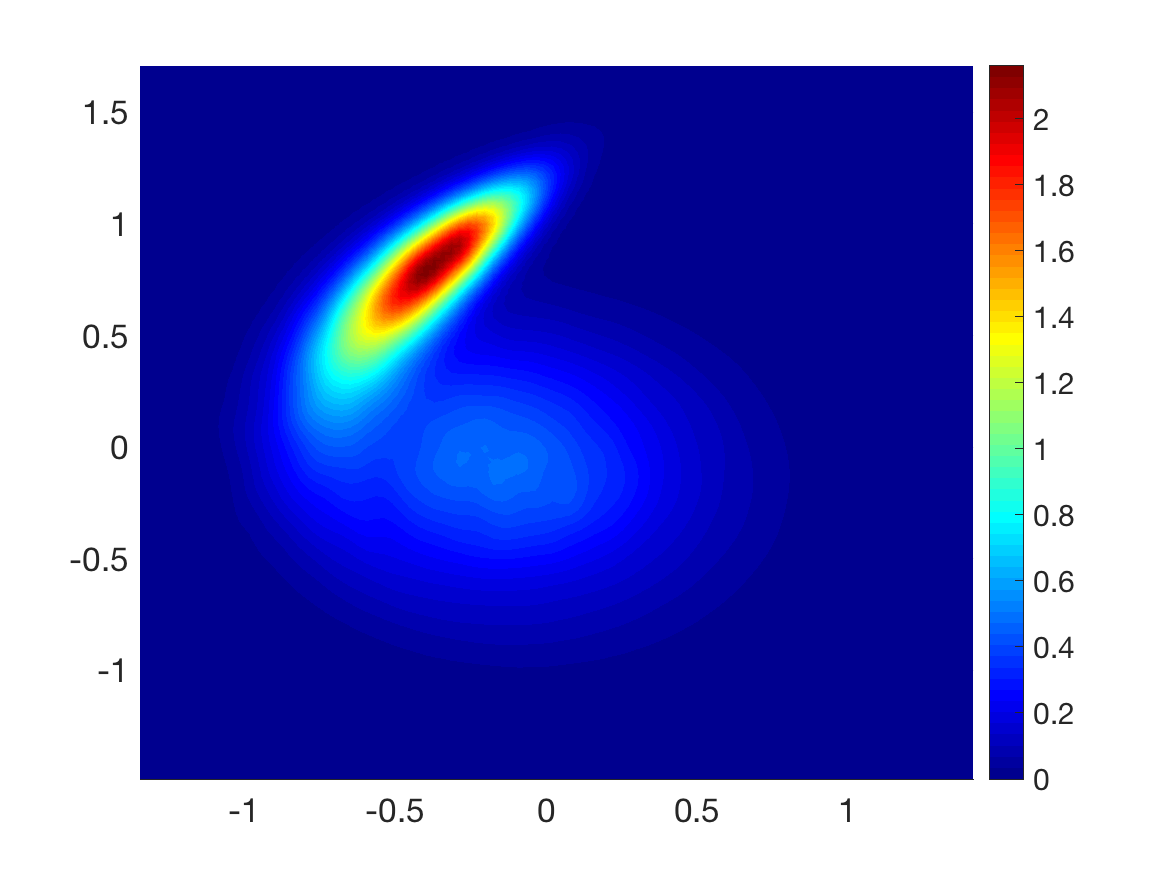
\includegraphics[width=\textwidth]{plots/climate_model/h01/pdf2d_data_05_01.png}
		%\caption{$y=x$}
	\end{subfigure}
	\hfill
	\begin{subfigure}[b]{0.32\textwidth}
		\centering
		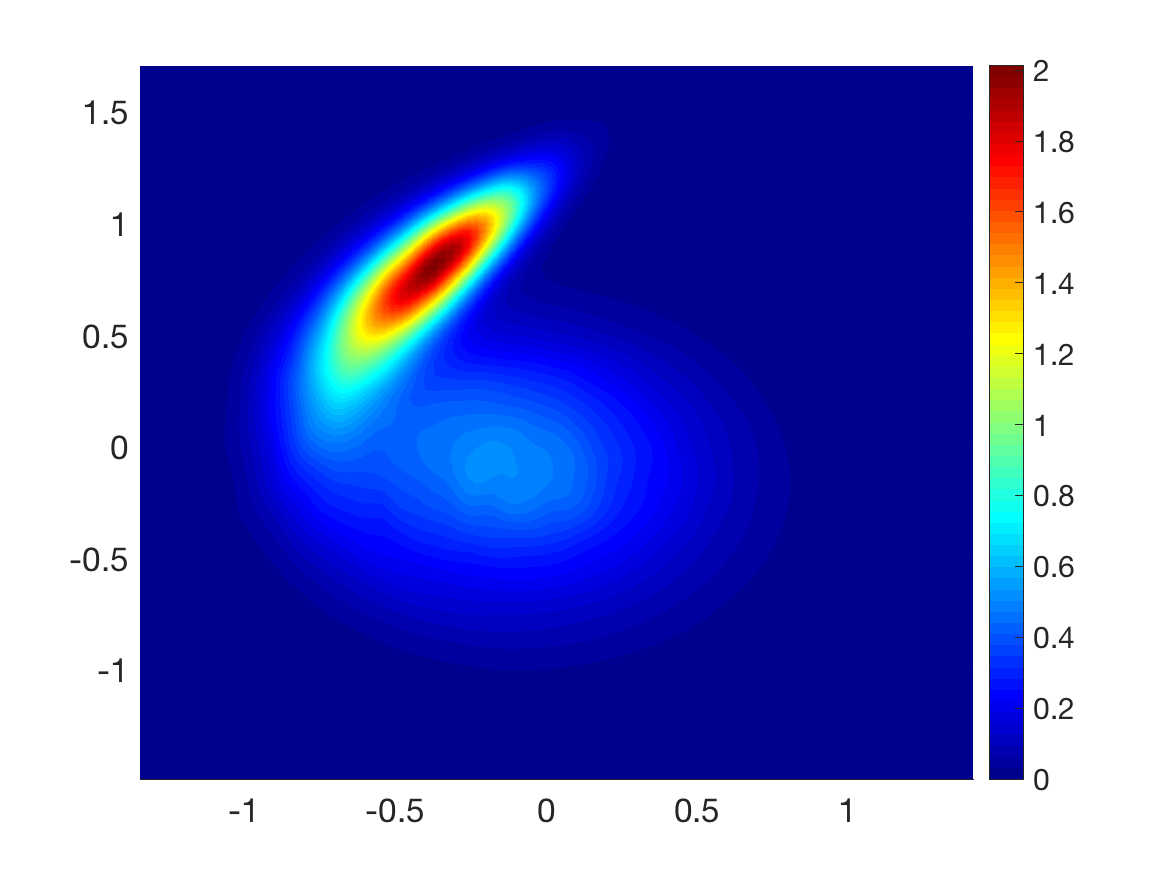
\includegraphics[width=\textwidth]{plots/climate_model/h01/pdf2d_emr_05_01.png}
		%\caption{$y=3sinx$}
	\end{subfigure}
	\hfill
	\begin{subfigure}[b]{0.32\textwidth}
		\centering
		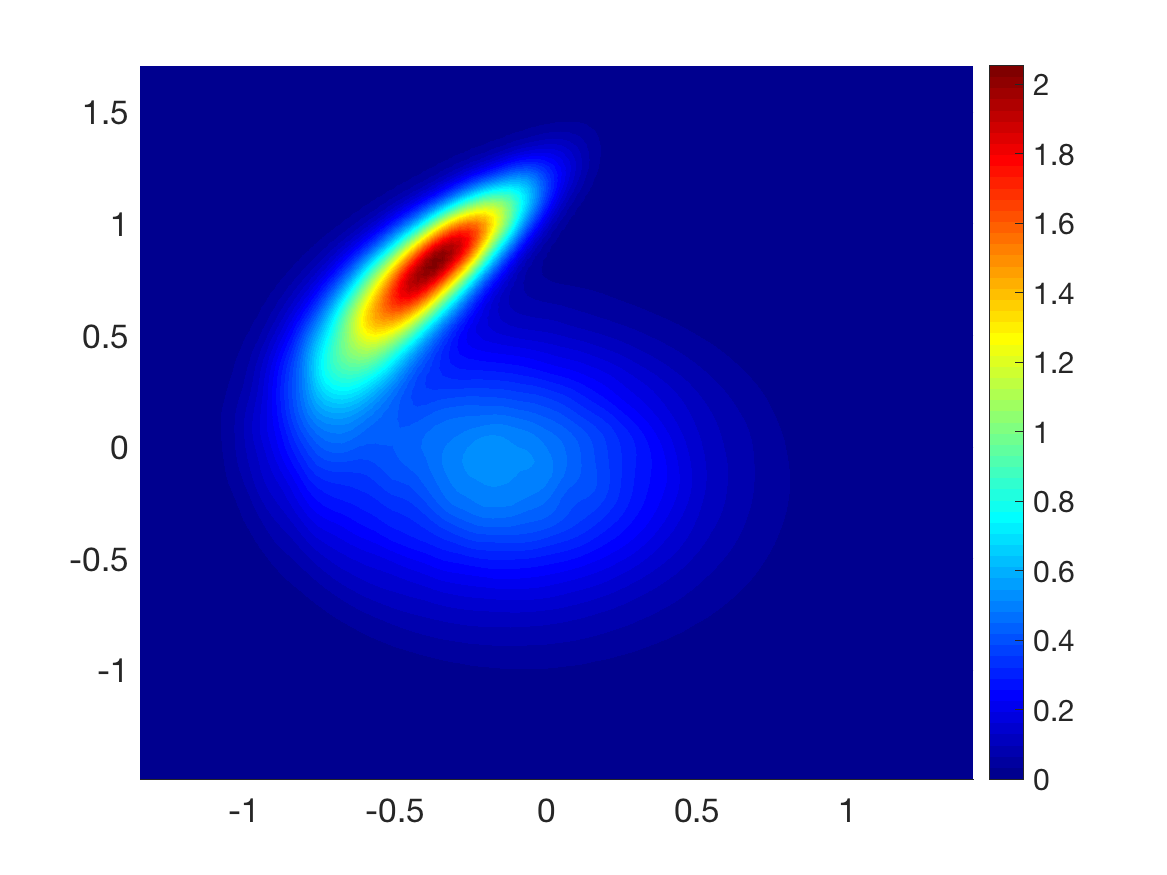
\includegraphics[width=\textwidth]{plots/climate_model/h01/pdf2d_wl_05_01.png}
		%\caption{$y=3sinx$}
	\end{subfigure}
	\caption{\label{climatologies 1}Two dimensional PDFs of the stochastic model obtained with the full integration (left) an integration of the EMR model (middle) and the WL parametrisation (right).}
\end{figure}

\begin{figure}[H]
	\centering
	\begin{subfigure}[b]{0.49\textwidth}
		\centering
		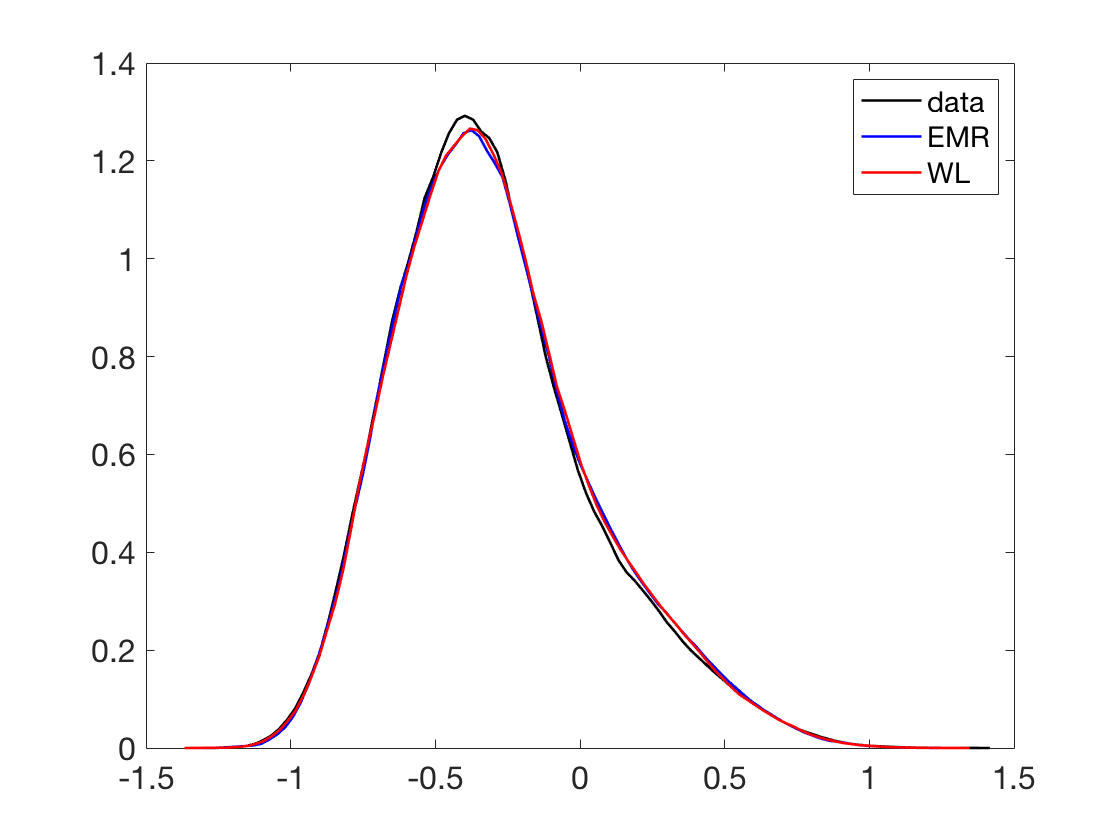
\includegraphics[width=\textwidth]{plots/climate_model/h01/pdfx1_e05_h01.png}
		%\caption{$y=5/x$}
	\end{subfigure}
	\begin{subfigure}[b]{0.49\textwidth}
		\centering
		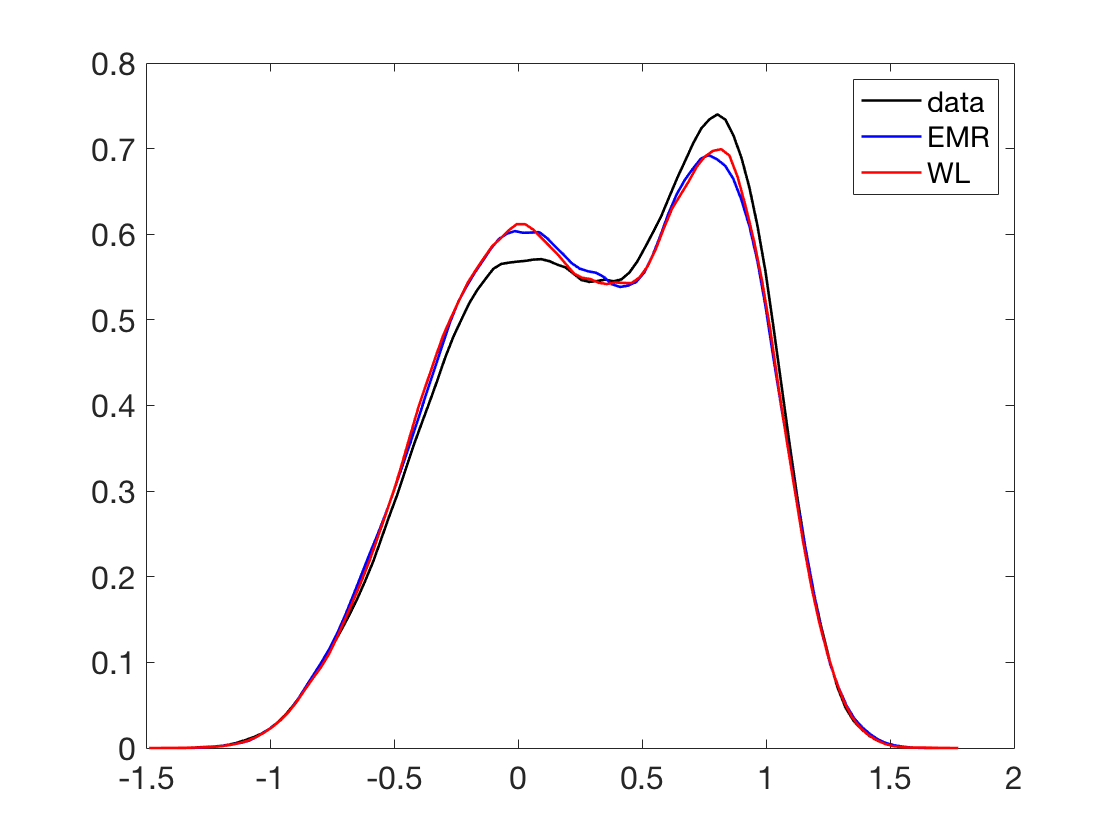
\includegraphics[width=\textwidth]{plots/climate_model/h01/pdfx2_e05_h01.png}
		%\caption{$y=5/x$}
	\end{subfigure}
	\caption{PDFs of the $x_1$ variable (left) and $x_2$ variable (right). These are obtained with the methods indicated on the plot.}
\end{figure}

\begin{figure}[H]
	\centering
	\begin{subfigure}[b]{0.49\textwidth}
		\centering
		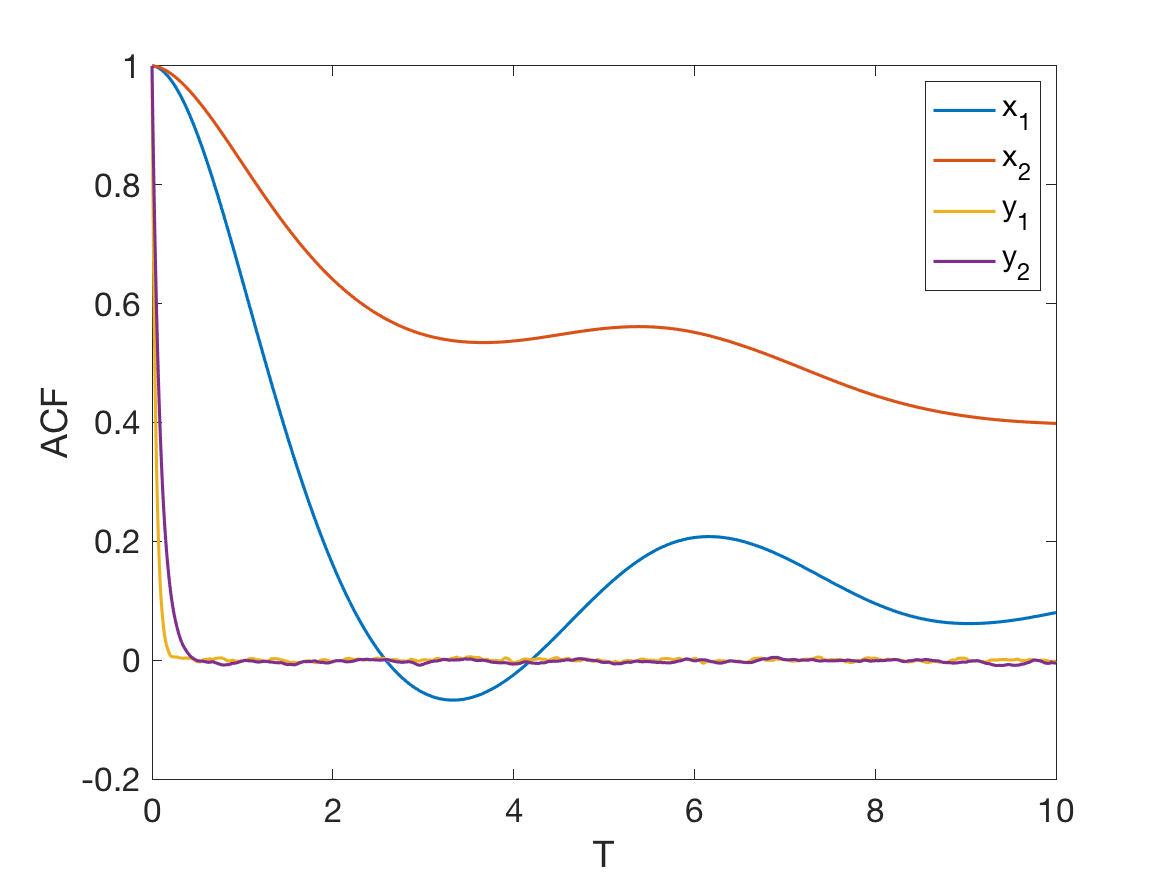
\includegraphics[width=\textwidth]{plots/climate_model/h01/acf_data_05_01.png}
		%\caption{$y=5/x$}
	\end{subfigure}
	\begin{subfigure}[b]{0.49\textwidth}
		\centering
		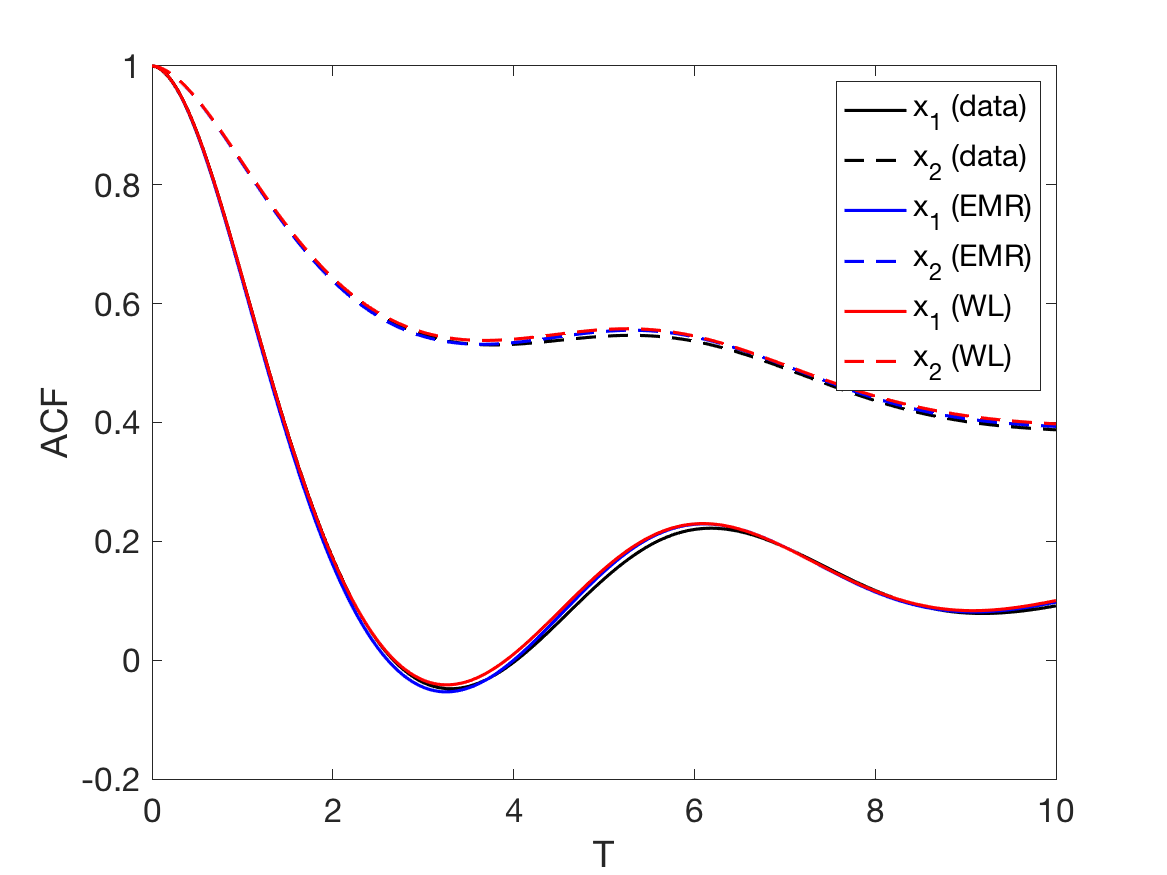
\includegraphics[width=\textwidth]{plots/climate_model/h01/acf_e05_h01.png}
		%\caption{$y=5/x$}
	\end{subfigure}
	\caption{\label{correlations 1}Autocorrelation functions for the four variables obtained from the full model (left) and the comparison of those obtained with the EMR model and WL parametrisation (right).}
\end{figure}

In general, and by referring to \cite{Kravtsov2005}, the regressions performed in the main level of the EMR model allows for effectively reconstructing the coefficients of a weakly coupled model (see Appendix B and C). However, the nonlinear couplings considered here compromised the estimation of the main model parameters, as expected. The model coefficients are as shown in these tables:

\begin{table}[H]
\centering
\caption{Empirically estimated EMR model coefficients at the first level.}
\begin{tabular}{cccccc}
	$F$ & $x_1$ & $x_2$ & $x_1^2$ & $x_1x_2$ & $x_2^2$ \\ 
	\hline 
	-0.31404 & -0.50954 & -0.065313 & 0 & -1.0092 & 0.99704 \\ 
	-0.15356 & 0.12353 & 0.21979 & 1.0092 & -0.99704 & 0 \\ 
	\hline 
\end{tabular}
\end{table}

\begin{table}[H]
	\centering
	\caption{Empirically estimated EMR model coefficients at the second level.}
\begin{tabular}{ccccc}
	$F^{(1)}$ & $x_1$ & $x_2$ & $r^{(1)}_1$ & $r^{(1)}_2$  \\ 
	\hline 
0 & -5.6397e-4 & -6.9382e-05 & -20.2823 & 0.016165  \\ 
0 & -1.648e-4 & -4.72e-4 & 0.086621 & -10.0426  \\ 
	\hline 
\end{tabular}
\end{table}

As we discussed in the previous section, the EMR has the structure of an MSM and it can be recast into an integro-differential equation. If one only considers the first two levels, the EMR can be readily integrated giving the following equation for the evolution of the slow variables $\xx = (x_1,x_2)$:
\begin{equation}\label{intdiff equation}
d\xx(t) =\FFF (\xx(t)) + e^{-\mathrm{D}t}\yy (0) + \int _{0}^te^{-\mathrm{D}(t-s)} \Sigma \dd \mathbf{W}_s + \int _{0}^{t}e^{-\mathrm{D}(t-s)}\mathrm{C}\xx(s)\dd s,
\end{equation}
where here,
\begin{align}
	&\mathrm{D}=\begin{bmatrix}
	-19.9982 & 2.1122\cdot 10^{-3}  \\ 
	-0.77528 & -10.116
	\end{bmatrix}, \mathrm{C}=\begin{bmatrix}
	-5\cdot 10^{-3} & -5\cdot 10^{-4}\\
	-1\cdot 10^{-3} & -5\cdot 10^{-3} 
	\end{bmatrix}, 
\\
	&\Sigma =\begin{bmatrix}
	0.2626 & -0.0014  \\ 
	-0.0014 & 0.5013
	\end{bmatrix}.
\end{align}
First thing to note is that the matrix $\mathrm{C}$ is small and, by virtue of Eq.~(\ref{intdiff equation}), it means that memory effects are going to be very small. Still, were such matrix be large, the eigenvalues of the matrix $\mathrm{D}$ are $\lambda _1 \approx -20$ and $\lambda _2 \approx -10$, which are approximatelly the drift coefficients of the uncoupled Ornstein-Uhlenbeck process driving the uncoupled $\yy$-variables. This indicates that the exponential kernel is, indeed, damping the effects of the $\xx$-variables in past times: the further away in time, the smaller the contribution. Moreover the covariance matrix $\Sigma$ corresponds to that obtained by integrating the $\yy$-dynamics independently, by comparison to Eq.~({\ref{covariance matrix wl}}).

\subsection{Reduced time-scale separation }

The parameter $h$ controls the time scale separation in the motion of the $\xx$ and $\yy$-variables. Here we set $h=1$ so that such separation is reduced by an order of magnitude as illustrated by the autocorrelation functions in Figure \ref{autocorrelations epsilon 1}. The question to be addressed in the subsection is the effects of reduction of time-scale separatioin in the parametrisations and their performance.

With regards to the WL parametrisation, one has to notice that there is no need of sampling the dynamics to construct it, since the formulas given in such theory are readily adaptable to any value of $h$. Hence, the covariance matrix and time-correlations of the WL noise correction is exactly given by Eq.~(\ref{autocorrelation function wl}). The memory term is expected to change as the kernel will decay more slowly by a factor of $10$. Therefore, memory effects are more relevant, as expected.

The EMR approach on the other hand needs to be learned, again, from a partial observations of the system when $h=1$. In the first level regression (see Table \ref{table coeffs emr l1 epsilon 1}), one observes that the parameter values differ substantially to those estimated in the previous case, distancing even more from the original ones. The covariance matrix of the noise correction is indicated in Eq.~\ref{cov mat emr epsilon 1}, agreeing to large extent with the previous case's. The memory kernel possesses exponential decay proportional to the drift coefficents in the decoupled Ornstein-Uhlenbeck processes governing the hidden physics. Before, we noted that the matrix  $\mathrm{C}$ indicates the strength of the memory effects. To our suprise, in spite of having less time-scale separation between the equations, the magnitude of such matrix is of the same order. This tells us that the loss of Markovianity might be intrinsic to the nature of the coupling rather than the time-scale separation, even if in the imit case memory effects will dissapear.

The performance of both parametrisation techniques is summarised in figures \ref{histograms 2d epsilon 1}, \ref{pdf 2} and \ref{autocorrelations epsilon 1}. First, we note that in this scenario there is no strict time-scale separation, as indicated by the autocorrelation functions obtained from the full model. Secondly, none of the approaches seem to be affected by the time-scale reduction. Indeed, the obtained projected densities and their two-dimensional analogues math the, still, non-Gaussian reference.

 Regarding the structure of the models, the memory kernels posses the same decay rates and the properties of the noise are approximately the same. These decay rates correspond, as in the previous case, to the drift cocefficients in the uncoupled $\yy$-dynamics.

\begin{figure}[H]
	\centering
	\begin{subfigure}[b]{0.32\textwidth}
		\centering
		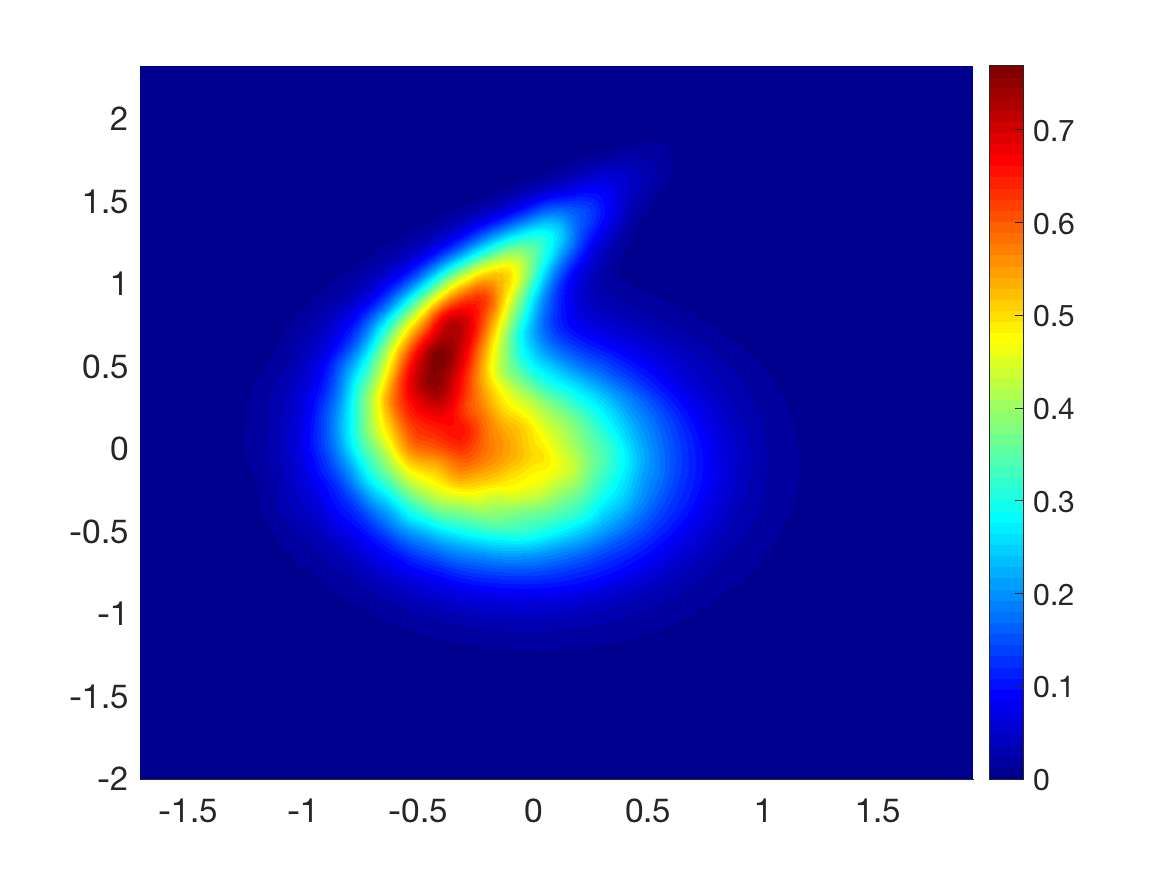
\includegraphics[width=\textwidth]{plots/climate_model/h1/pdf2d_data_e05_h1.png}
		%\caption{$y=x$}
	\end{subfigure}
	\hfill
	\begin{subfigure}[b]{0.32\textwidth}
		\centering
		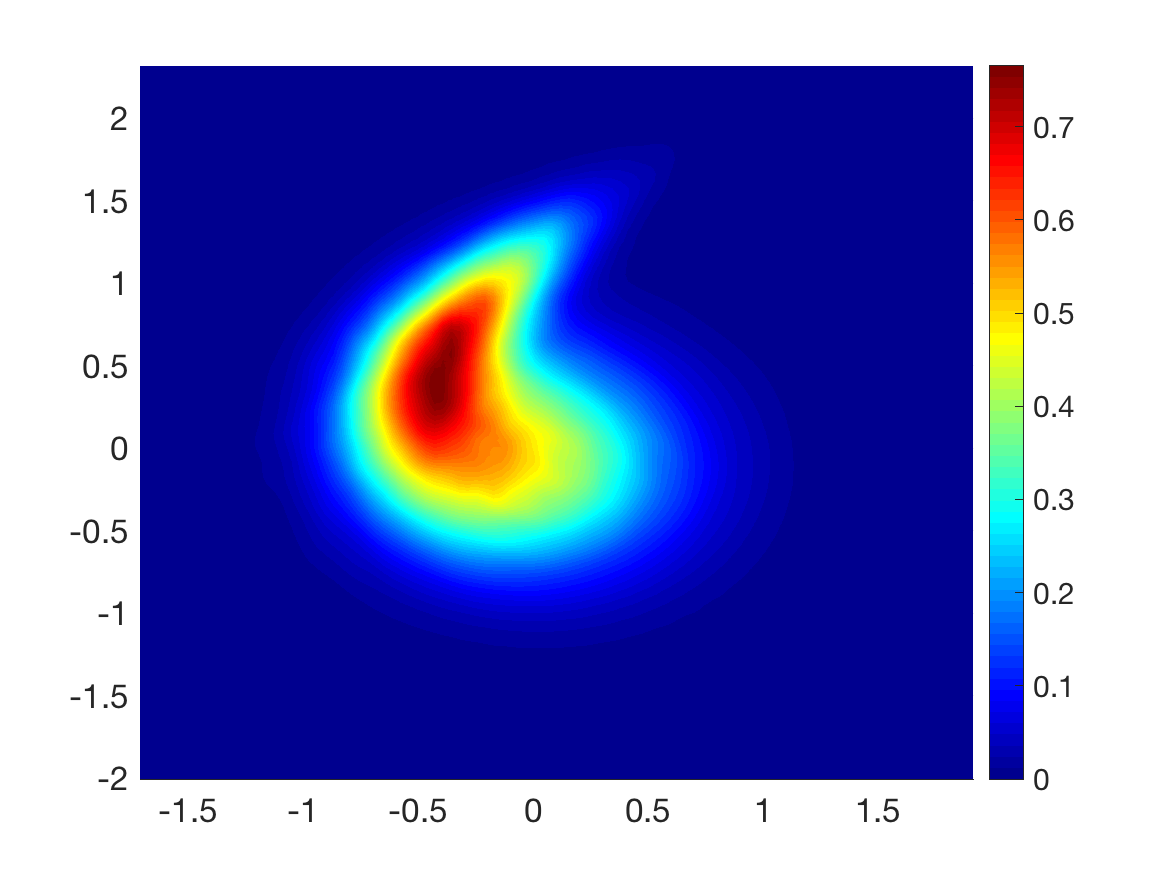
\includegraphics[width=\textwidth]{plots/climate_model/h1/pdf2d_emr_e05_h1.png}
		%\caption{$y=3sinx$}
	\end{subfigure}
	\hfill
	\begin{subfigure}[b]{0.32\textwidth}
		\centering
		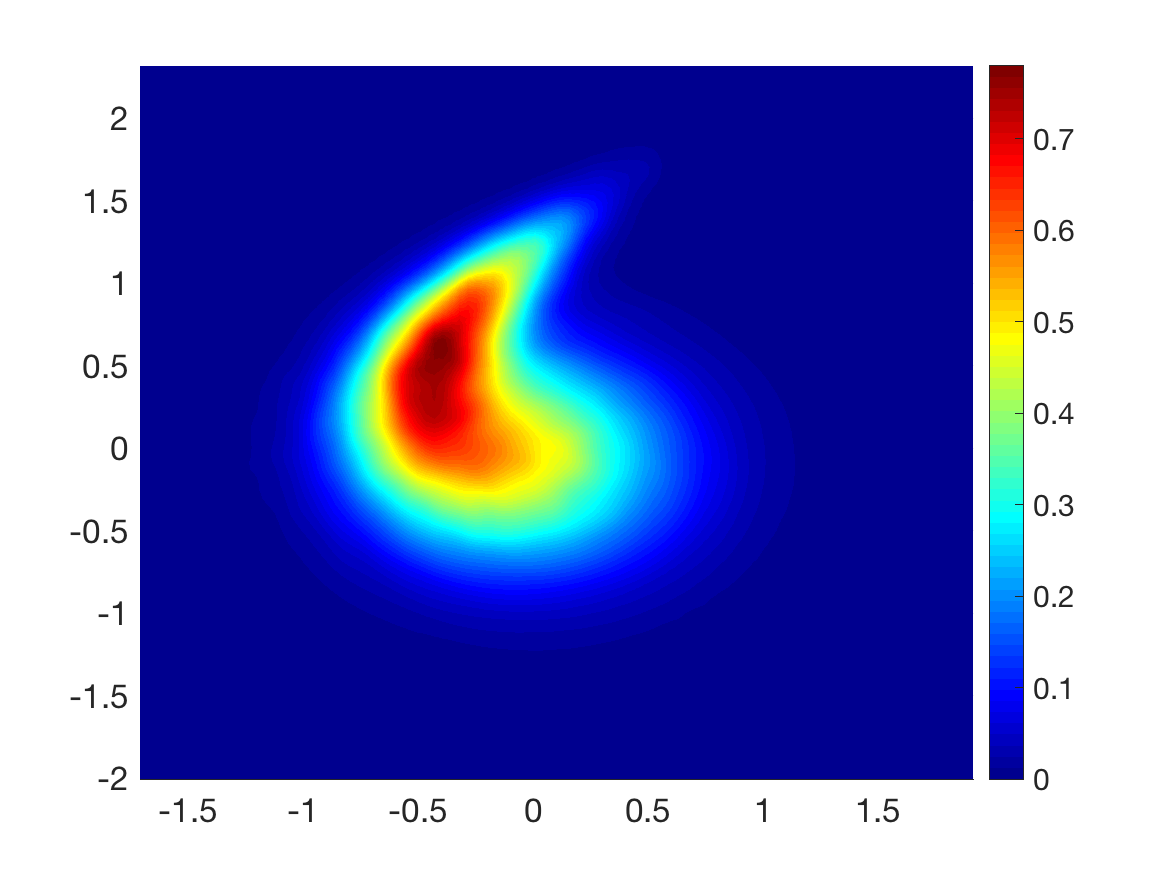
\includegraphics[width=\textwidth]{plots/climate_model/h1/pdf2d_wl_e05_h1.png}
		%\caption{$y=3sinx$}
	\end{subfigure}
	\caption{\label{histograms 2d epsilon 1}Two dimensional PDFs of the stochastic model obtained with the full integration (left), EMR model (middle) and WL parametrisation (right).}
\end{figure}

\begin{figure}[H]
	\centering
	\begin{subfigure}[b]{0.49\textwidth}
		\centering
		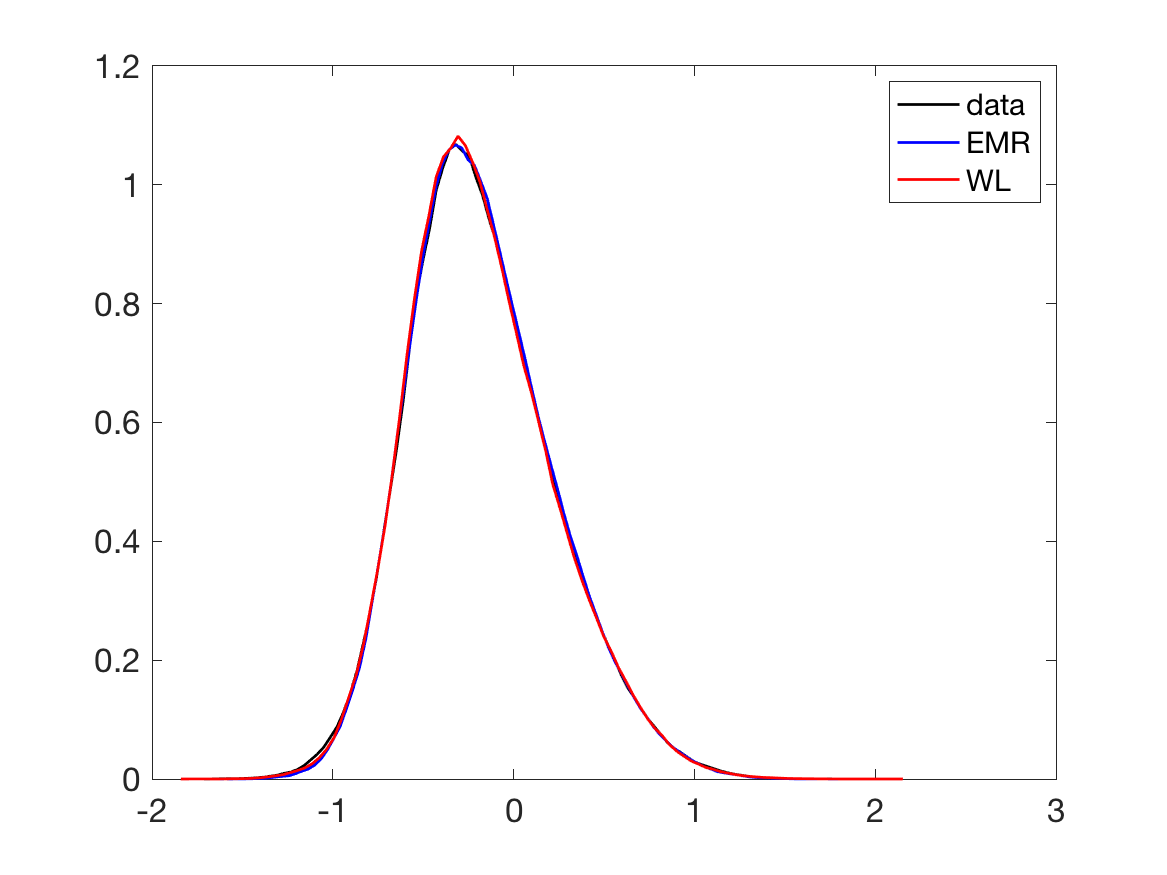
\includegraphics[width=\textwidth]{plots/climate_model/h1/pdfx1_e05_h1.png}
		%\caption{$y=5/x$}
	\end{subfigure}
	\begin{subfigure}[b]{0.49\textwidth}
		\centering
		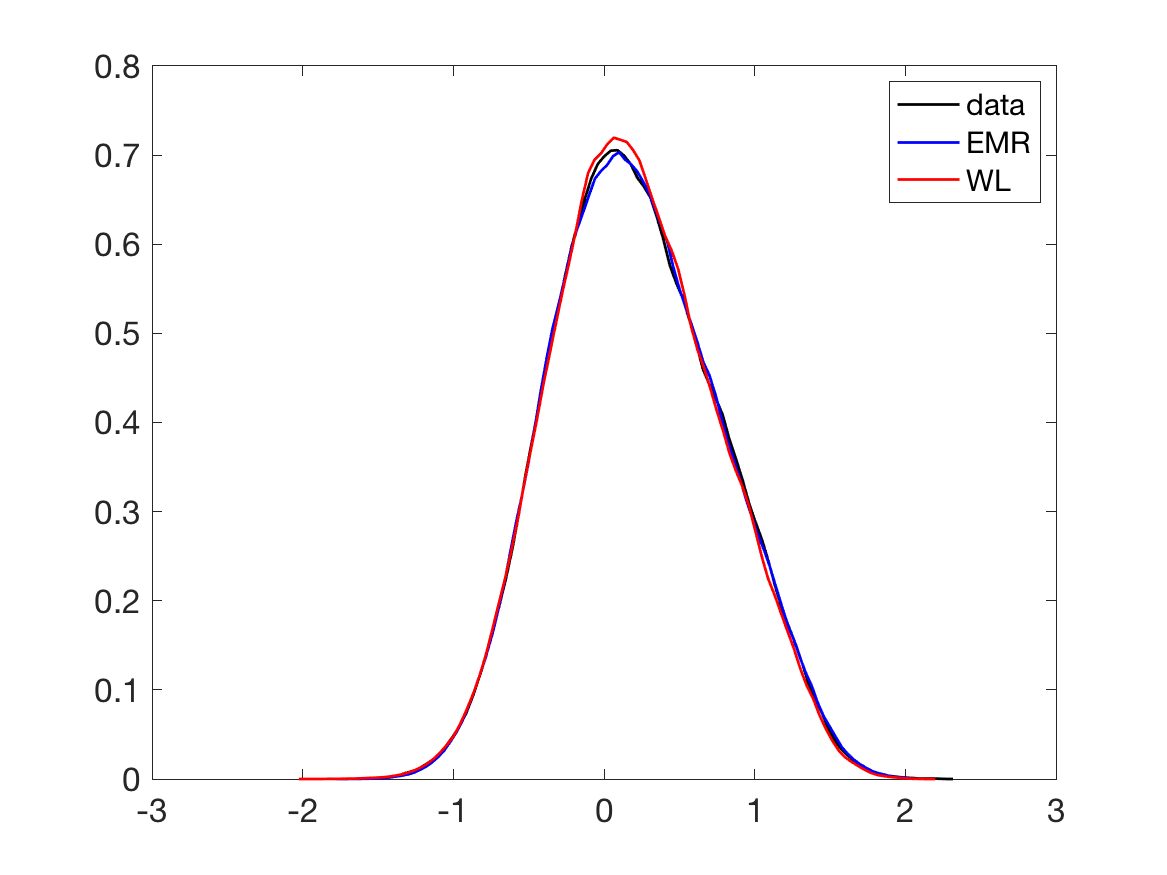
\includegraphics[width=\textwidth]{plots/climate_model/h1/pdfx2_e05_h1.png}
		%\caption{$y=5/x$}
	\end{subfigure}
	\caption{\label{pdf 2}PDFs of the $x_1$ variable (left) and $x_2$ variable (right). These are obtained with the methods indicated on the plot.}
\end{figure}

\begin{figure}[H]
	\centering
	\begin{subfigure}[b]{0.49\textwidth}
		\centering
		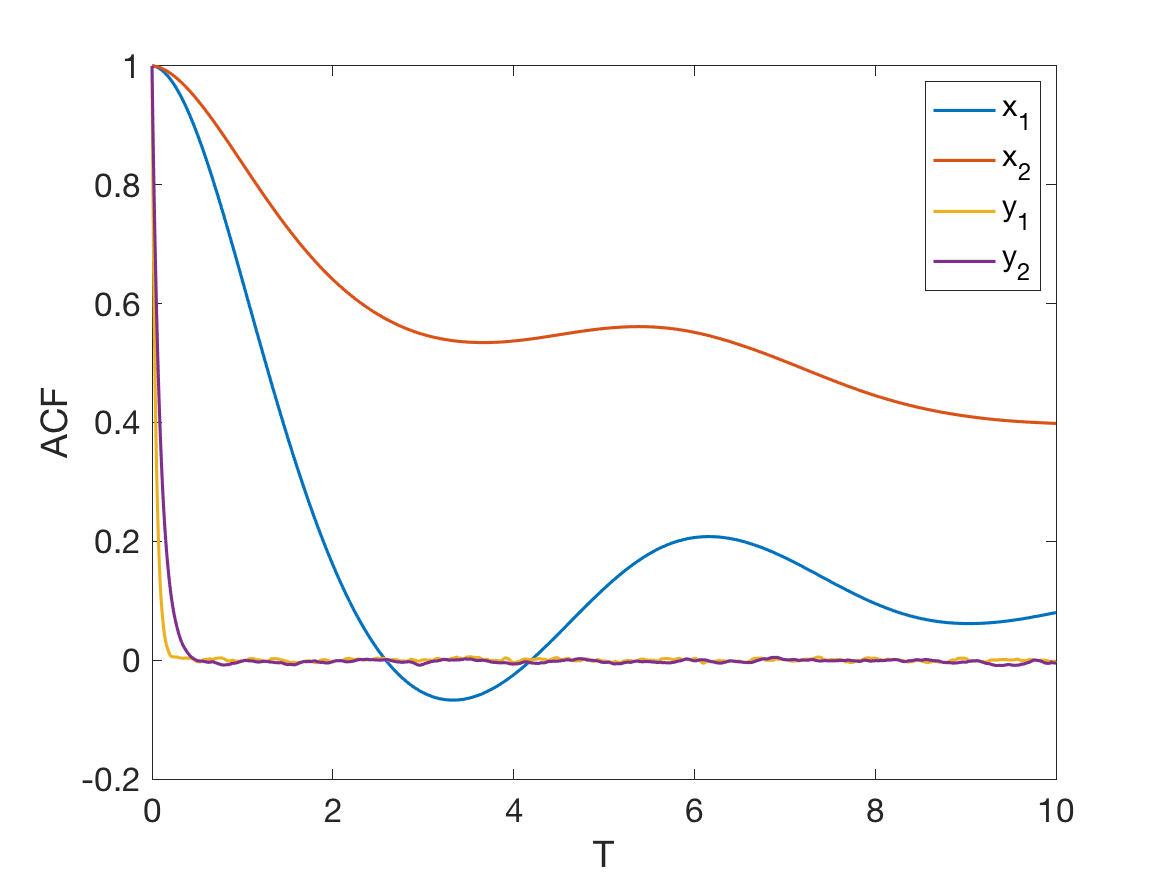
\includegraphics[width=\textwidth]{plots/climate_model/h01/acf_data_05_01.png}
		%\caption{$y=5/x$}
	\end{subfigure}
	\begin{subfigure}[b]{0.49\textwidth}
		\centering
		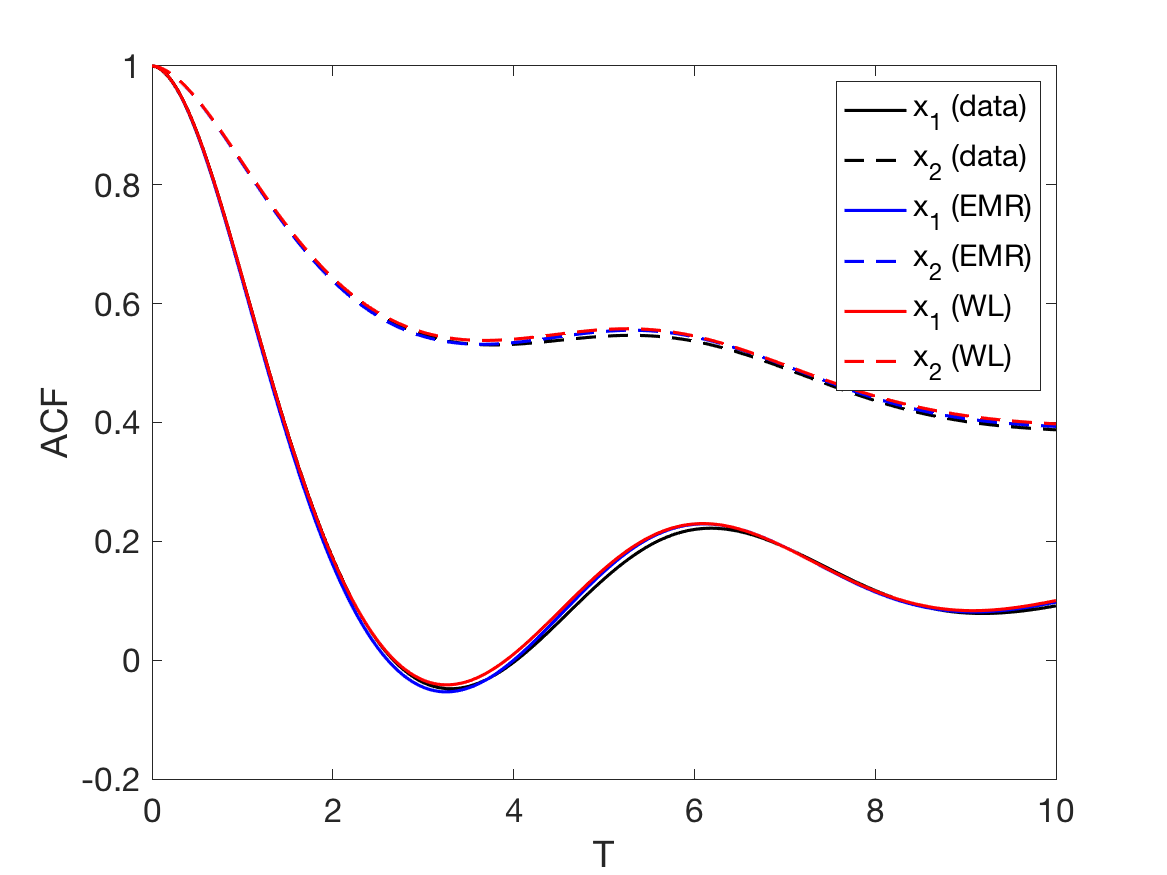
\includegraphics[width=\textwidth]{plots/climate_model/h01/acf_e05_h01.png}
		%\caption{$y=5/x$}
	\end{subfigure}
	\caption{\label{autocorrelations epsilon 1}Autocorrelation functions for the four variables obtained from the full model (left) and the comparison of those obtained with the EMR model and WL parametrisation (right).}
\end{figure}

\begin{table}[H]
	\centering
	\caption{\label{table coeffs emr l1 epsilon 1}Empirically estimated EMR model coefficients at the first level.}
	\begin{tabular}{cccccc}
		$F$ & $x_1$ & $x_2$ & $x_1^2$ & $x_1x_2$ & $x_2^2$ \\ 
		\hline 
-0.31181 & -0.339 & -0.42944 & 0 & -0.93439 & 0.97958 \\ 
-0.16925 & 0.46833 & 0.17513 & 0.93439 & -0.97958 & 0 \\ 
		\hline 
	\end{tabular}
\end{table}

\begin{table}[H]
	\centering
	\caption{Empirically estimated EMR model coefficients at the second level.}
	\begin{tabular}{ccccc}
		$F^{(1)}$ & $x_1$ & $x_2$ & $r^{(1)}_1$ & $r^{(1)}_2$  \\ 
		\hline 
0 & -3.9452e-3 & -1.5027e-4 & -2.1001 & 0.016509  \\ 
0 & -5.0312e-4 & -3.79e-3 & 0.054861 & -1.1214  \\ 
		\hline 
	\end{tabular}
\end{table}


\begin{align}
	&\mathrm{D}=\begin{bmatrix}
-2.1001 & 0.016509  \\ 
0.054861 & -1.1214 
	\end{bmatrix} , \mathrm{C}=\begin{bmatrix}
-4\cdot 10^{-3} & -1\cdot 10^{-4} \\
-6\cdot 10^{-4} & -4\cdot 10^{-3}
	\end{bmatrix}, 
	\\\label{cov mat emr epsilon 1}
	&\Sigma =\begin{bmatrix}
	0.2618 & 0.0011  \\ 
	0.0011 & 0.4554
	\end{bmatrix}.
\end{align}

\subsection{Memory Effects}

We would like to end the results section by analysing the relevance of the memory effects when performing a reduction of the model given by Eqs.~(\ref{stochastic model 1})-(\ref{stochastic model 4}). For that we would like to apply the criterion discussed in Section \ref{memory effects subsection}. For that, we spectrally approximated the autocorrelation functions of the variables $x_1$ and $x_2$ using Eq.~({\ref{criterion memory effects}}) with the Koopman operator $\mathcal{T}_{\tau}$ estimated using Ulam's method with a time-lag of $\tau=0.5$ time units for the case where $h=0.1$ and $\tau=1$ time-unit for $h=1$. We clearly observe in Figure \ref{autocorrelations transfer operator} that the correlation functions can be accurately reconstructed in the case of large-timescale separation $h=0.1$ and not so for $h=1$. This indicates, naturally, that memory effects are negligible in the first case and relevant in the second.
\begin{figure}[H]
	\centering
	\begin{subfigure}[b]{0.49\textwidth}
		\centering
		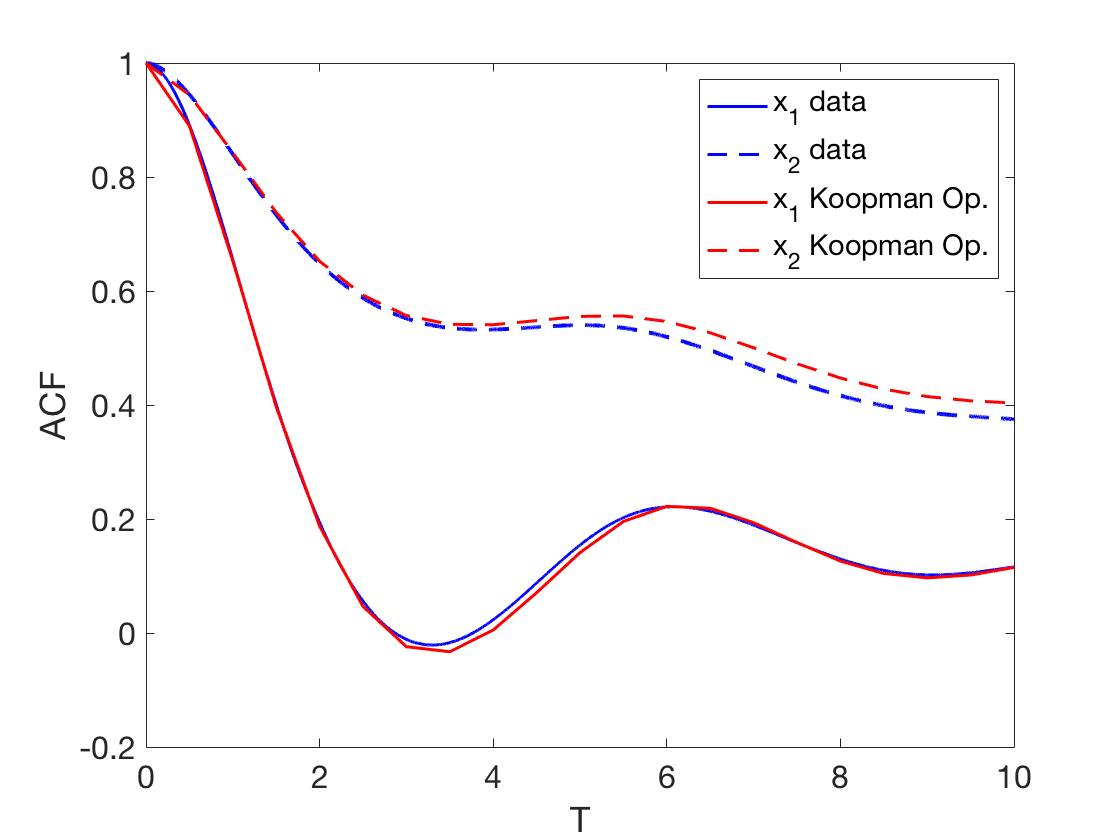
\includegraphics[width=\textwidth]{plots/climate_model/h1/corr_top_e1.png}
		%\caption{$y=5/x$}
	\end{subfigure}
	\begin{subfigure}[b]{0.49\textwidth}
		\centering
		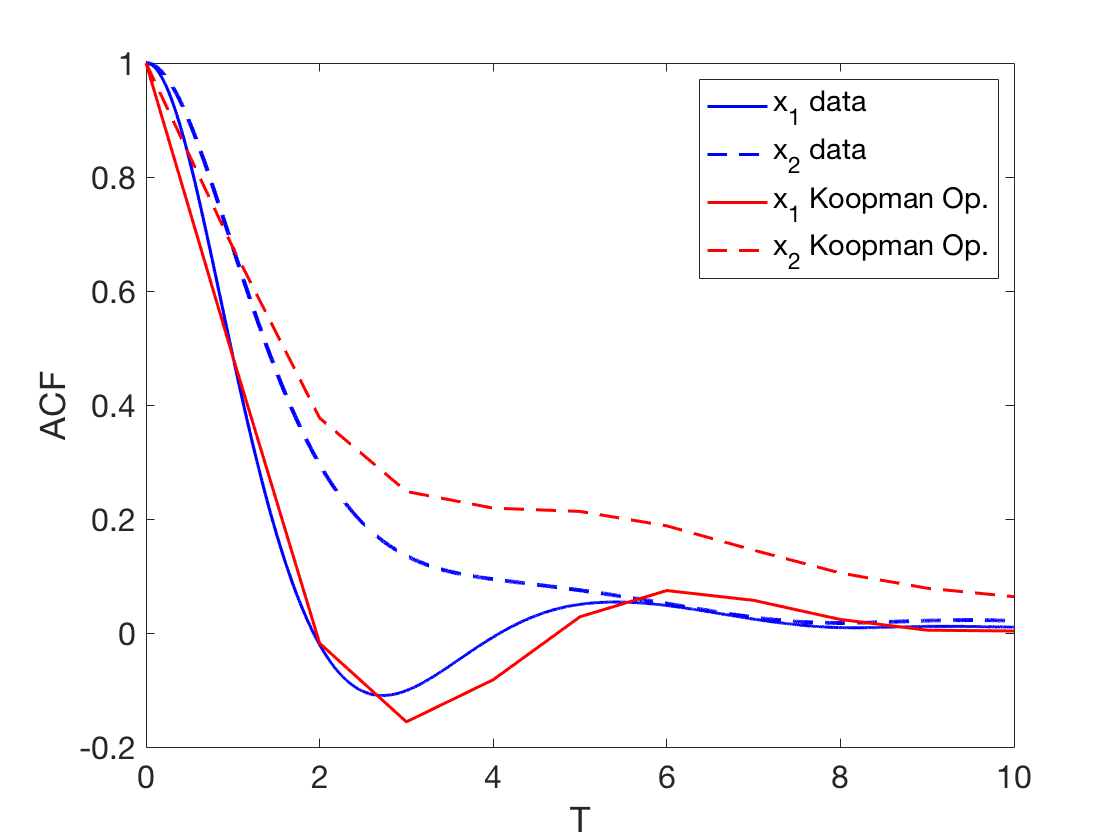
\includegraphics[width=\textwidth]{plots/climate_model/h01/corr_top_e01.png}
		%\caption{$y=5/x$}
	\end{subfigure}
	\caption{\label{autocorrelations transfer operator}Autocorrelation functions for $\xx$-variables obtained from the full model (left) the spectral reconstruction using the Kooman operator. The left image shows the case for $h=0.1$ and the one on the right shows the case where $h=1$.}
\end{figure}

\section*{Summary/Discussion}

In this document we have revisited the foundations of the WL parametrisation presented originally in  \cite{Wouters2012, wouters2013}. As noted in previous work, the Dyson formalism appears to be essential to determine the effects of the hidden processes as a result of coupling them to the observed variables, when working at the level of observables. In fact, this methodology is explicit, in the sense that no information about the coupled process is needed. Indeed, by only possessing an ensemble of the hidden variables, one can identify the components of the parametrisation. This calculation was originally performed for the additively coupled system; here we extended for separable coupling functions.

Another advantage of this approach is that it can be implemented for any arbitrary time-scale separation in an adaptable way, again, as noted in previous work \cite{Vissio2018a}. In particular, the presence of a time-scale separation parameter in the equation for the hidden variables would modify the speed at which the memory kernel decays; as a simple calculation would suggest.

We address the problem of re-Markovianising the WL memory equation, as pointed out in \cite{Wouters2016}, where authors showed that a re-Markovianisation can lead to a Markovian system with, still, fewer degrees of freedom than the original one. Here we give a framework to be able to perform such re-Markovianisation. The assumptions boil down to having a good spectral decomposition of the Koopman operator for the hidden variables.

In the second half of the document we explore MSM which have been shown to be susceptible to approximate the GLE predicted by Mori and Zwanzig. First, we show that a seemless application of the WL parametrisation solves the MSM coinciding with its Ito integration. Second, it is reminded how an MSM can be obtained from partial observations of the coupled system, namely, the EMR approach. This methodology is dual to that of the WL parametrisation in the sense that only partial observations of the coupled systems are required.

Finally, we consider a conceptual climate model to which both methodologies revisited in this document are applied. Since both the EMR and the WL parametrisation yield a memory equation involving integrals and stochastic noise, we were able to, not only compare the main statistical outputs, but also compare their structure. We found that both methodologies produced equivalent results and that the memory kernel and noise predicted in the WL parametrisation were reflected in the empirical approach.

In this document we have given further evidence an MSM is really susceptible of approximating the GLE predicted by the Mori-Zwanzig formalism. In other work, MSM are suggested as a good statistical/empirical/data-driven model for the evolution of observed variables. Here, on the other hand, we suggest that the MSM structure can be obtained from first principles by applying formal operator expansions to the Koopman operator.


\bibliography{progress_report} 
\bibliographystyle{abbrv}

\pagebreak

\section*{Appendix A: Ito integration of the MSM}

In the main text we proposed a solution of the MSM given by Eqs.~(\ref{msm1})-(\ref{msm2}) using the Dyson expansion for the linear operators involved in the backward Kolmogorov equation. There we worked at the level of observables where the action nonlinear flows can be understood as a linear advection acting on functions. Therefore, we substitute the nonlinear ODE for a PDE for the sake of having linear operators in hand. The same solution can be attained by using direct integrations of the MSM. Indeed, we can convolute (in the Ito sense) Eq.~(\ref{msm2}) to find an explicit solution for $\rr(t)$:
\begin{equation}
\rr (t) = e^{-\mathrm{D}t}\rr (0) + \int _{0}^te^{-\mathrm{D}(t-s)} \Sigma dW_s + \epsilon \int _{0}^{t}e^{-\mathrm{D}(t-s)}\mathrm{C}\xx(s)\dd s.
\end{equation}
where $\rr(0)$ indicates some initial condition which can also be regarded as distributed in a prescribed way. Hence, by inserting this expression into Eq.~(\ref{msm1}), we find an effective and exact expression for the time evolution for $\xx (t)$:
\begin{equation}
d\xx(t) =\FFF (\xx(t)) + \epsilon e^{-\mathrm{D}t}\rr (0) + \epsilon \int _{0}^te^{-\mathrm{D}(t-s)} \Sigma dW_s + \epsilon ^2 \int _{0}^{t}e^{-\mathrm{D}(t-s)}\mathrm{C}\xx(s)\dd s,
\end{equation}
where we inmediately find that the memory effects entailed by the fourth term are of second order in $\epsilon$. The first thing to underline is that the $\epsilon$-order terms concern a realisation of the noise in the decoupled regime, whereas the memory term is exclusively due to the coupling of the main variables with the hidden ones. Hence, the only degree of freedom left is the distribution of the initial condition $\rr(0)$.

\section*{Appendix B: The L63 System}

In this appendix, we consider the L63 model presented in \cite{lorenzdeterministic1963} as simple case of a low dimensional nonlinear model that displays chaotic dynamics on an attractor that supports an SRB measure arising from truncating the equation governing atmospheric convection. This set of equations has been used for a number of contexts within the climatological sciences for its simplicity but complete amount of dynamical features. 

With such model we would like to illustrate the validity of the EMR regression method as done previously \cite{Kravtsov2005, kondrashovdata2015}. The low-dimenionality of the system allows as to fully observe phase-space, so one should expect that errors committed in the regression only corresponds to perhaps a not-long-enough time series. In this section, we would like to answer the following questions:

\begin{enumerate}
	\item Can we approximate the coefficients of the system by only observing a time series? 
	\item If one includes an extra level in the EMR model, what is the observed (linear) interaction of the residual and the main level?
	\item Do we capture the main statistical properties: pdf's, autocorrelations and ergodicity spectrum?
\end{enumerate}
%One would hope an affirmative answer to (i), since one expects to recover the coefficients of the model as the time-resultion and length of the time-series increase. Question (ii) will test whether the EMR model introduces artificial interations between the residual and the current state. Note that since the time series is Markovian (in the sense that there is no time-subsampling), one expects to see no significant memory effects. Question (iii) aims at describing the nature of the correction noise. Again, since the time series is deterministic and Markovian, the decorrelation of the residuals should be fast and scale with the length of the time series and its resolution.


\begin{figure}[H]
	\centering
	\begin{subfigure}[b]{0.3\textwidth}
		\centering
		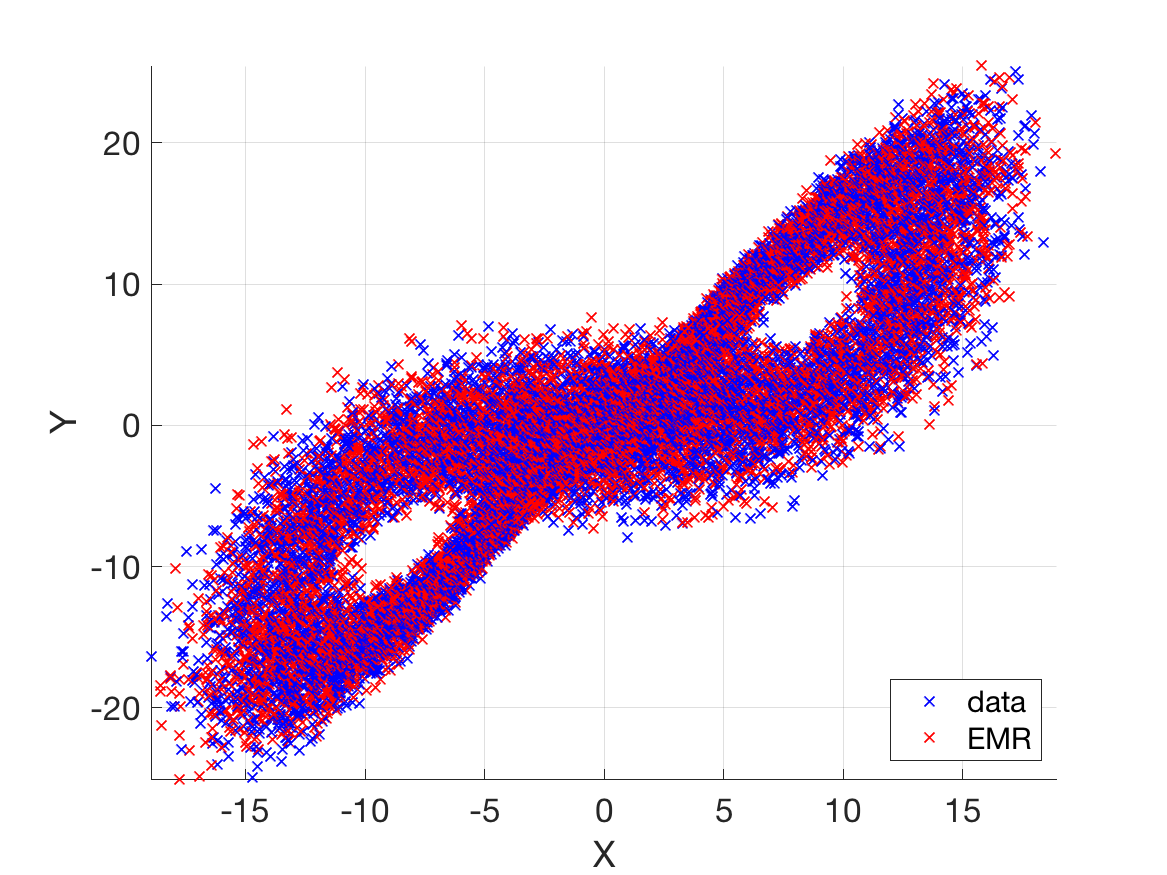
\includegraphics[width=\textwidth]{plots/l63/traj1.png}
		%\caption{$y=x$}
	\end{subfigure}
	\hfill
	\begin{subfigure}[b]{0.3\textwidth}
		\centering
		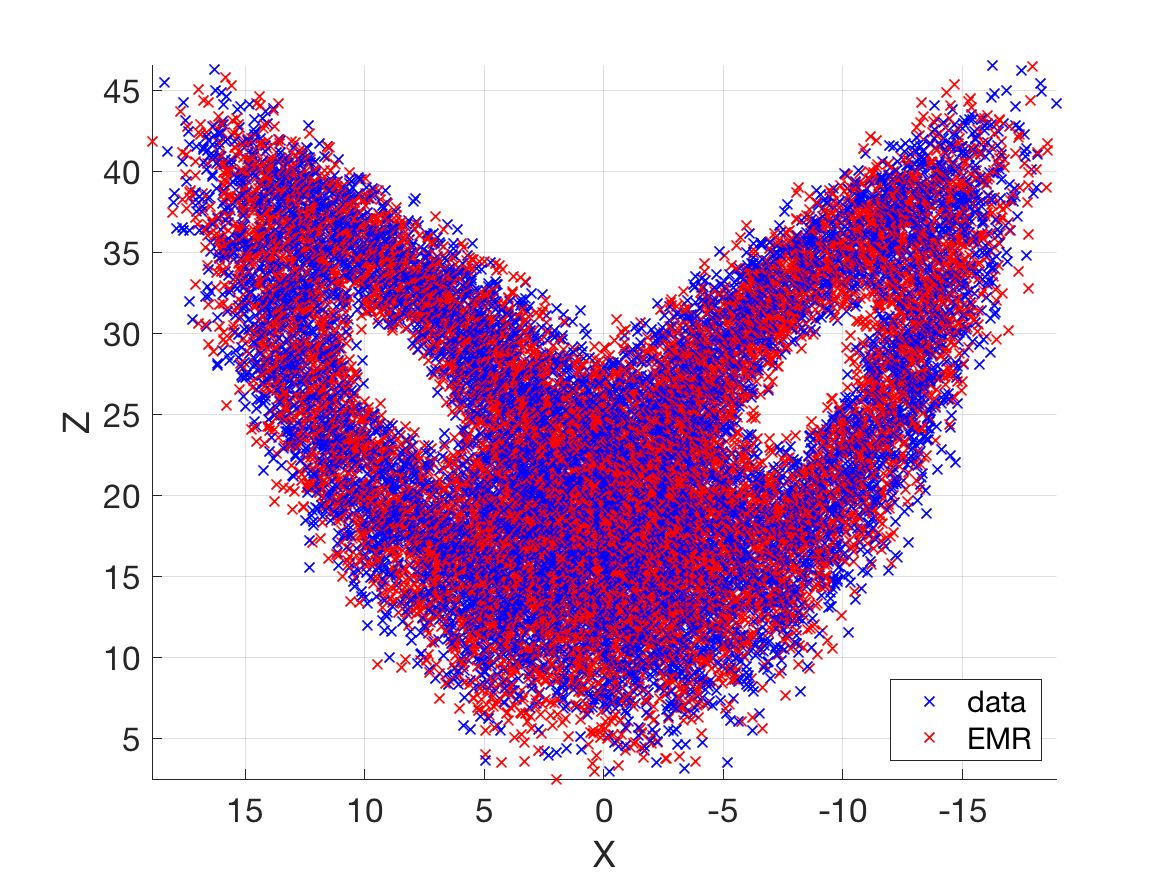
\includegraphics[width=\textwidth]{plots/l63/traj2.png}
		%\caption{$y=3sinx$}
	\end{subfigure}
	\hfill
	\begin{subfigure}[b]{0.3\textwidth}
		\centering
		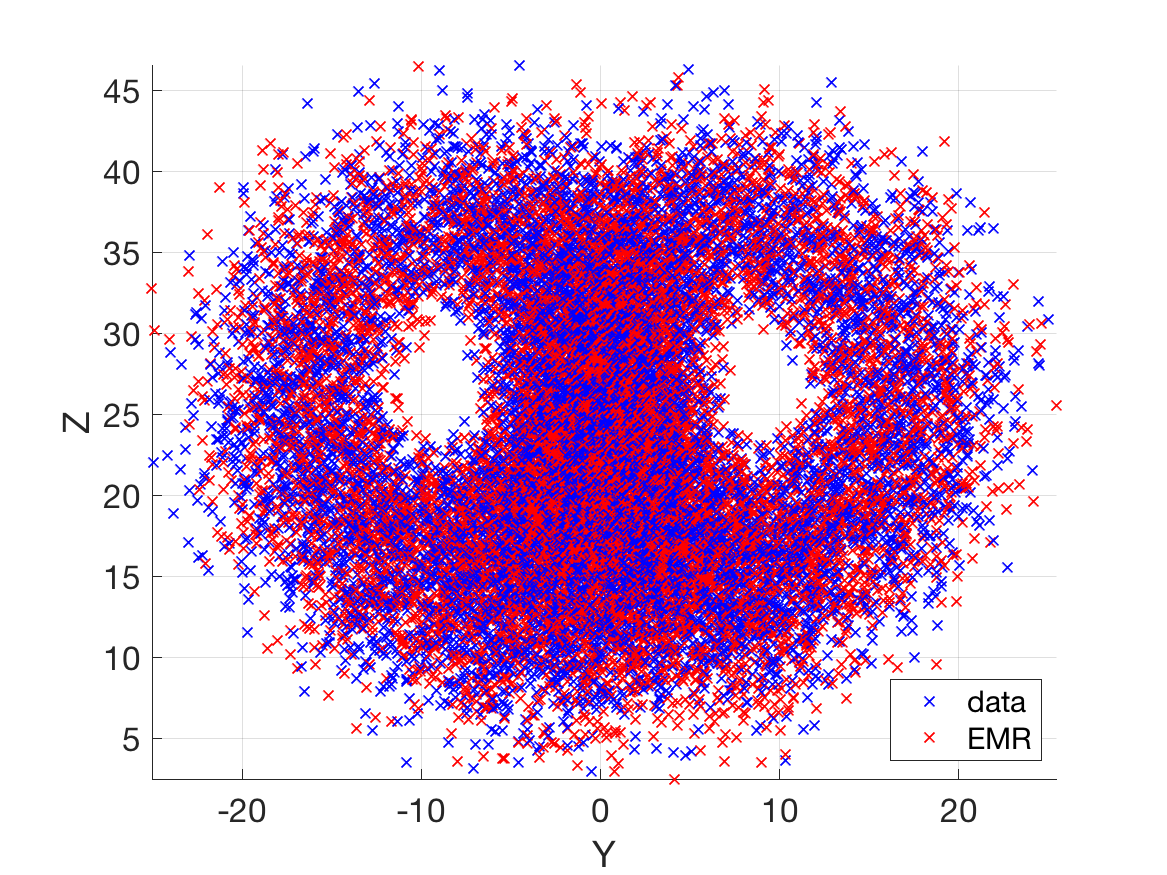
\includegraphics[width=\textwidth]{plots/l63/traj3.png}
		%\caption{$y=5/x$}
	\end{subfigure}
	\caption{Time-series plotted on phase space.}
\end{figure}


\begin{figure}[H]
	\centering
	\begin{subfigure}[b]{0.3\textwidth}
		\centering
		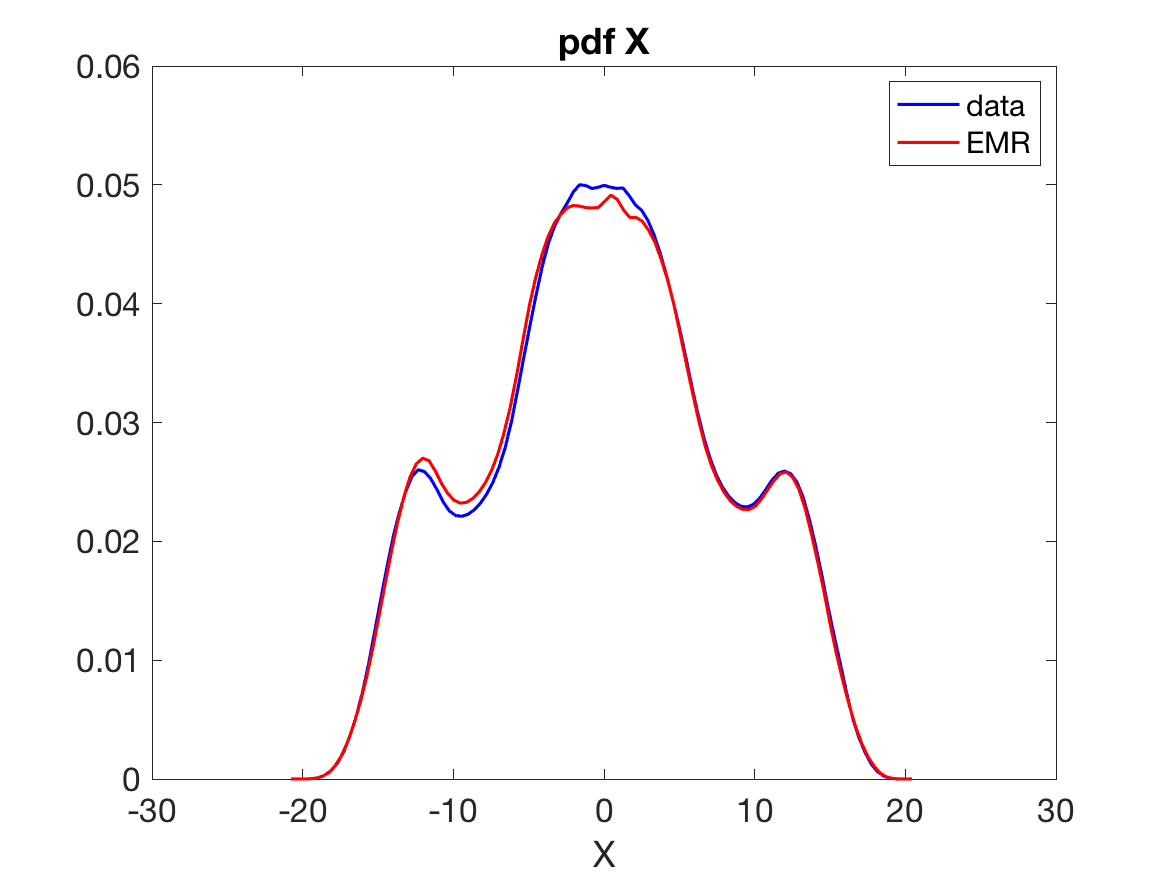
\includegraphics[width=\textwidth]{plots/l63/pdfxl63.png}
		%\caption{$y=x$}
	\end{subfigure}
	\hfill
	\begin{subfigure}[b]{0.3\textwidth}
		\centering
		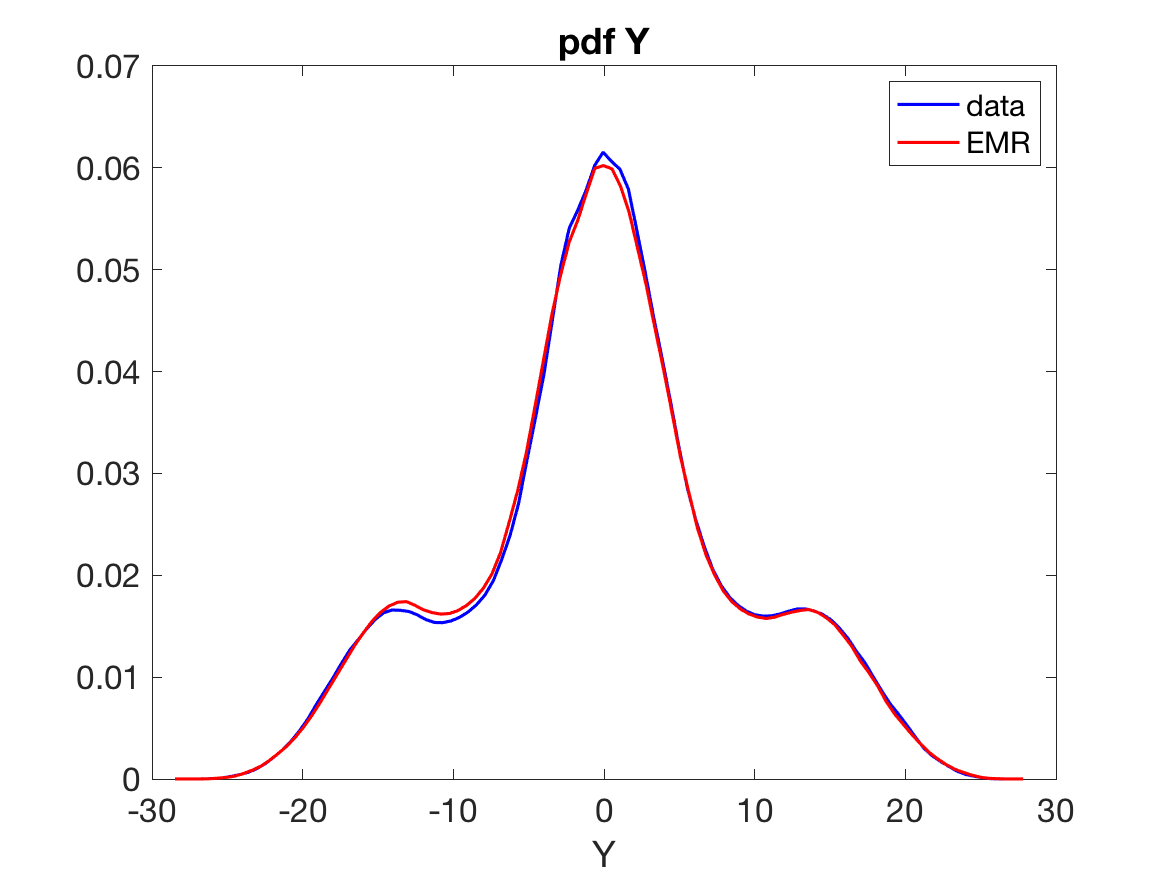
\includegraphics[width=\textwidth]{plots/l63/pdfyl63.png}
		%\caption{$y=3sinx$}
	\end{subfigure}
	\hfill
	\begin{subfigure}[b]{0.3\textwidth}
		\centering
		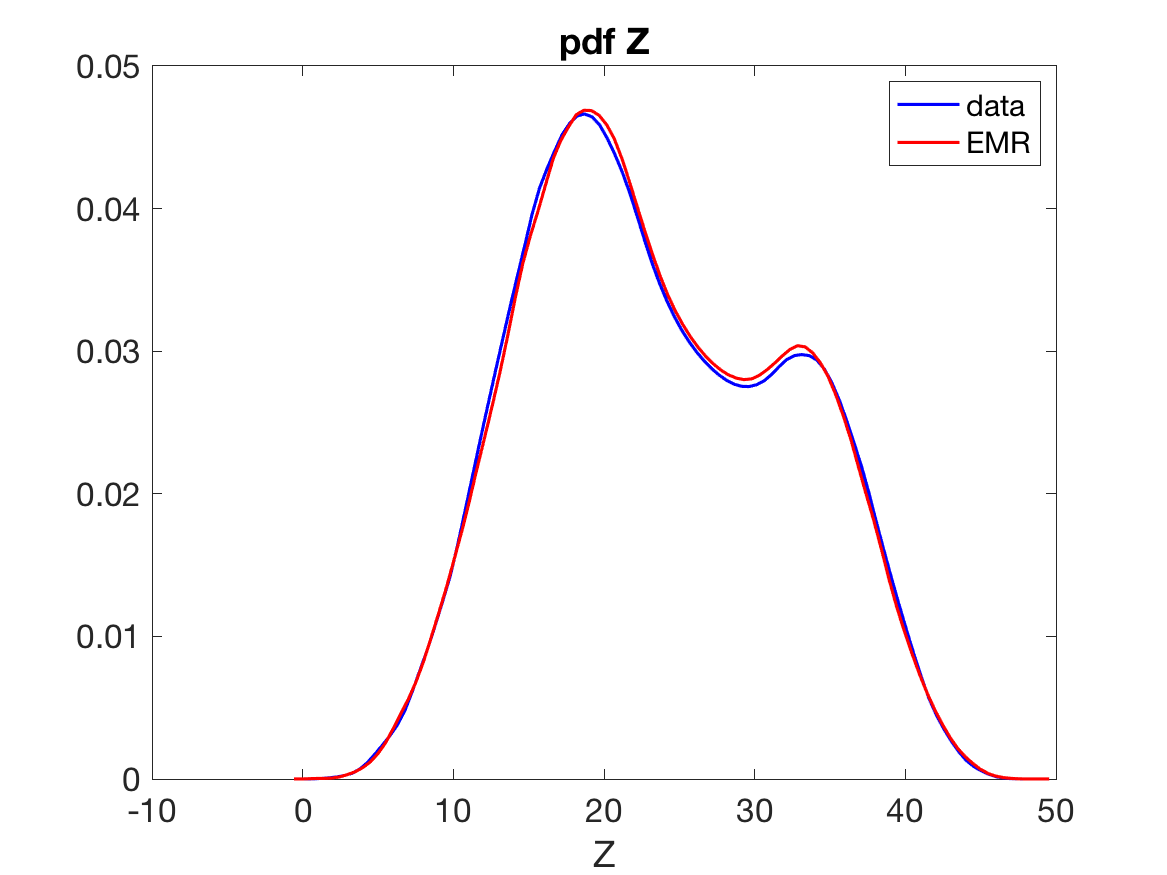
\includegraphics[width=\textwidth]{plots/l63/pdfzl63.png}
		%\caption{$y=5/x$}
	\end{subfigure}
	\caption{PDF's of L63.}
\end{figure}

\begin{figure}[H]
	\centering
	\begin{subfigure}[b]{0.3\textwidth}
		\centering
		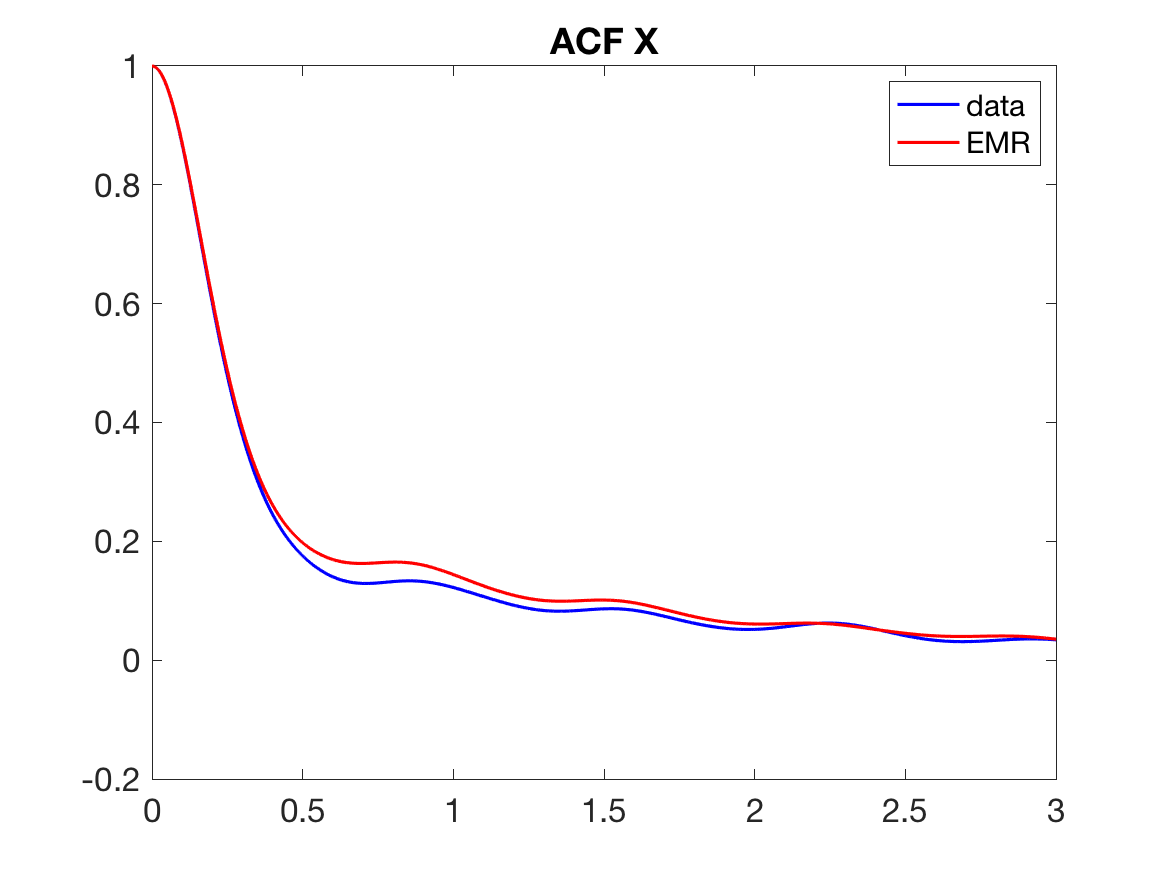
\includegraphics[width=\textwidth]{plots/l63/acfxl63.png}
		%\caption{$y=x$}
	\end{subfigure}
	\hfill
	\begin{subfigure}[b]{0.3\textwidth}
		\centering
		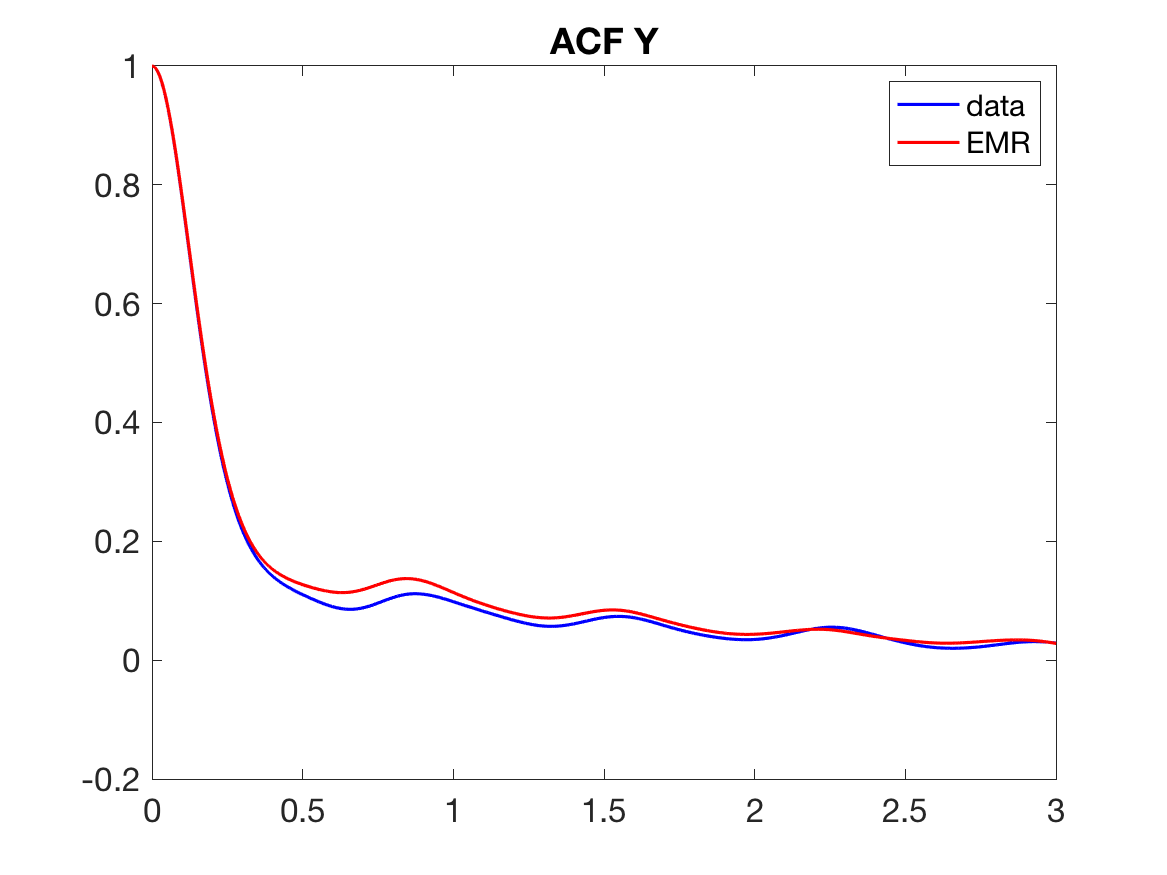
\includegraphics[width=\textwidth]{plots/l63/acfyl63.png}
		%\caption{$y=3sinx$}
	\end{subfigure}
	\hfill
	\begin{subfigure}[b]{0.3\textwidth}
		\centering
		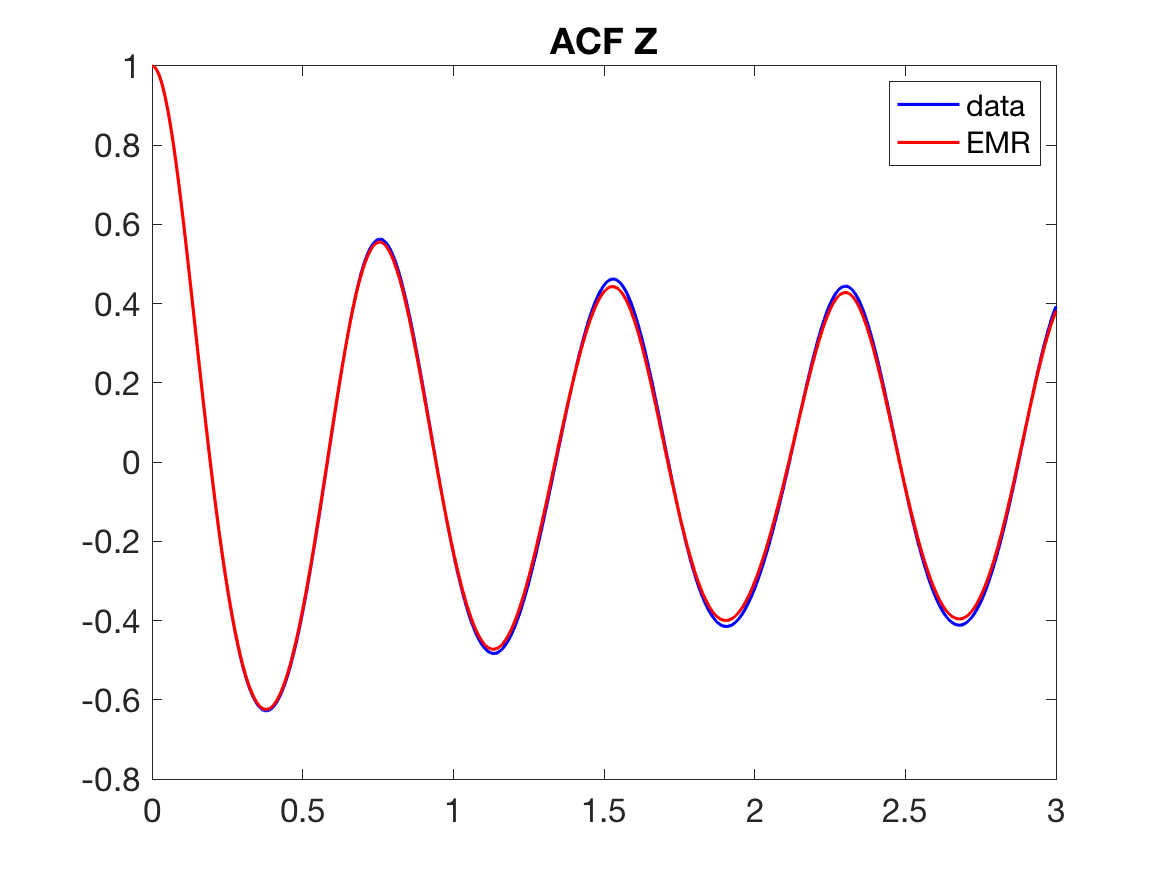
\includegraphics[width=\textwidth]{plots/l63/acfzl63.png}
		%\caption{$y=5/x$}
	\end{subfigure}
	\caption{Autocorrelation functions of L63.}
\end{figure}

\begin{figure}[H]
	\centering
	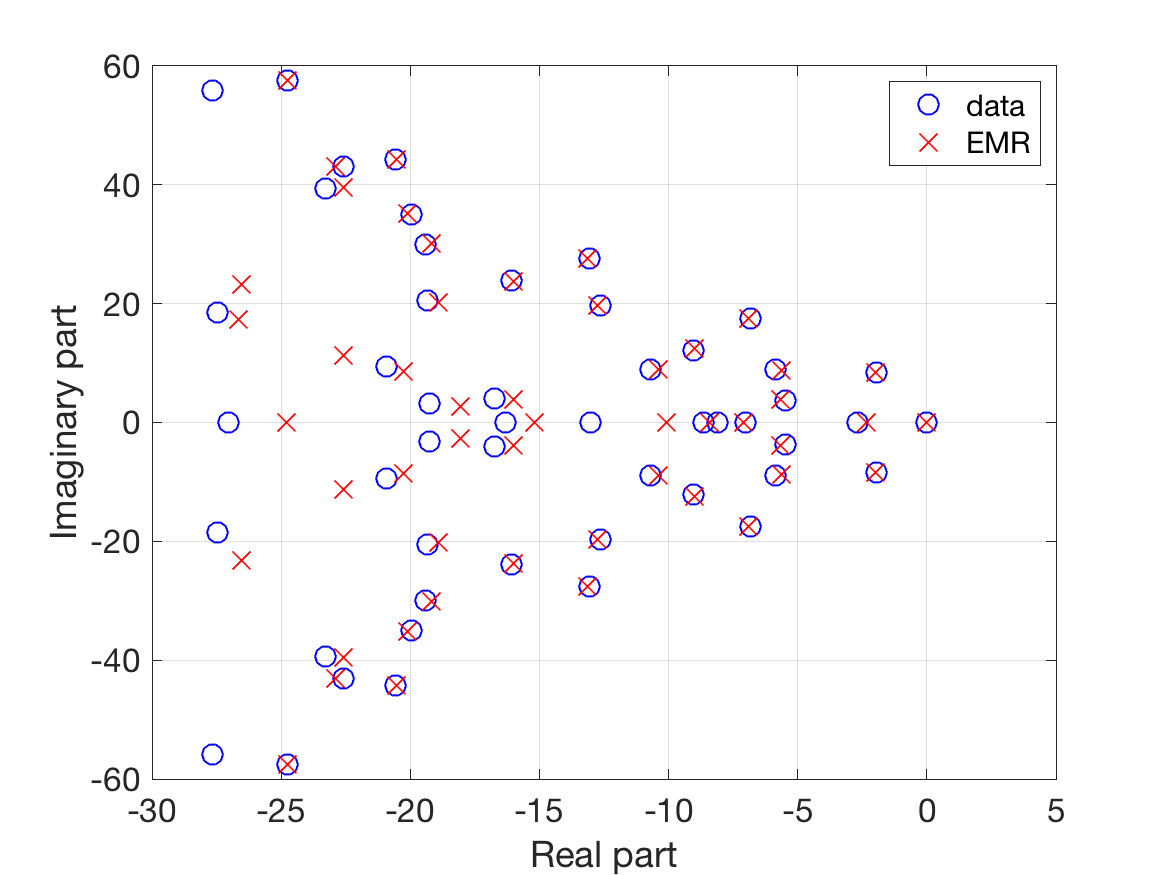
\includegraphics[width=\textwidth]{plots/l63/especl63.png}
	\caption{Observed ergodicity spectrum of L63.}
\end{figure}


\begin{table}[H]
	\centering
	\begin{tabular}{c | cccccccccc}
		EMR & $1$ & $x$ & $y$ & $z$ & $x^2$ & $xy$ & $y^2$ & $xz$ & $yz$ & $z^2$  \\ \hline
		$f_x$ & \hphantom{-}0.00 & -9.81 & \hphantom{-}9.95 & \hphantom{-}0.00 & \hphantom{-}0.00 &\hphantom{-}0.00 & \hphantom{-}0.00 & \hphantom{-}0.00 & \hphantom{-}0.00 & \hphantom{-}0.00 \\ 
		$f_y$ & \hphantom{-}0.00 & \hphantom{-}27.87 & -0.85 & \hphantom{-}0.00& \hphantom{-}0.00 & \hphantom{-}0.00 & \hphantom{-}0.00 & -0.99 &\hphantom{-}0.00 & \hphantom{-}0.00\\ 
		$f_z$ & -0.55 & \hphantom{-}0.00 & \hphantom{-}0.00 & -2.59 & \hphantom{-}0.00 & \hphantom{-}0.98 & \hphantom{-}0.01 & \hphantom{-}0.00& \hphantom{-}0.00 & \hphantom{-}0.00 \\ 
	\end{tabular}
	\caption{Means of the coefficients of L63 estimated on an ensemble of 20 runs. The standard deviations are not shown since the results were very robust.}
\end{table}


%\begin{figure}[H]
%	\centering
%	\begin{subfigure}[b]{0.45\textwidth}
%		\centering
%		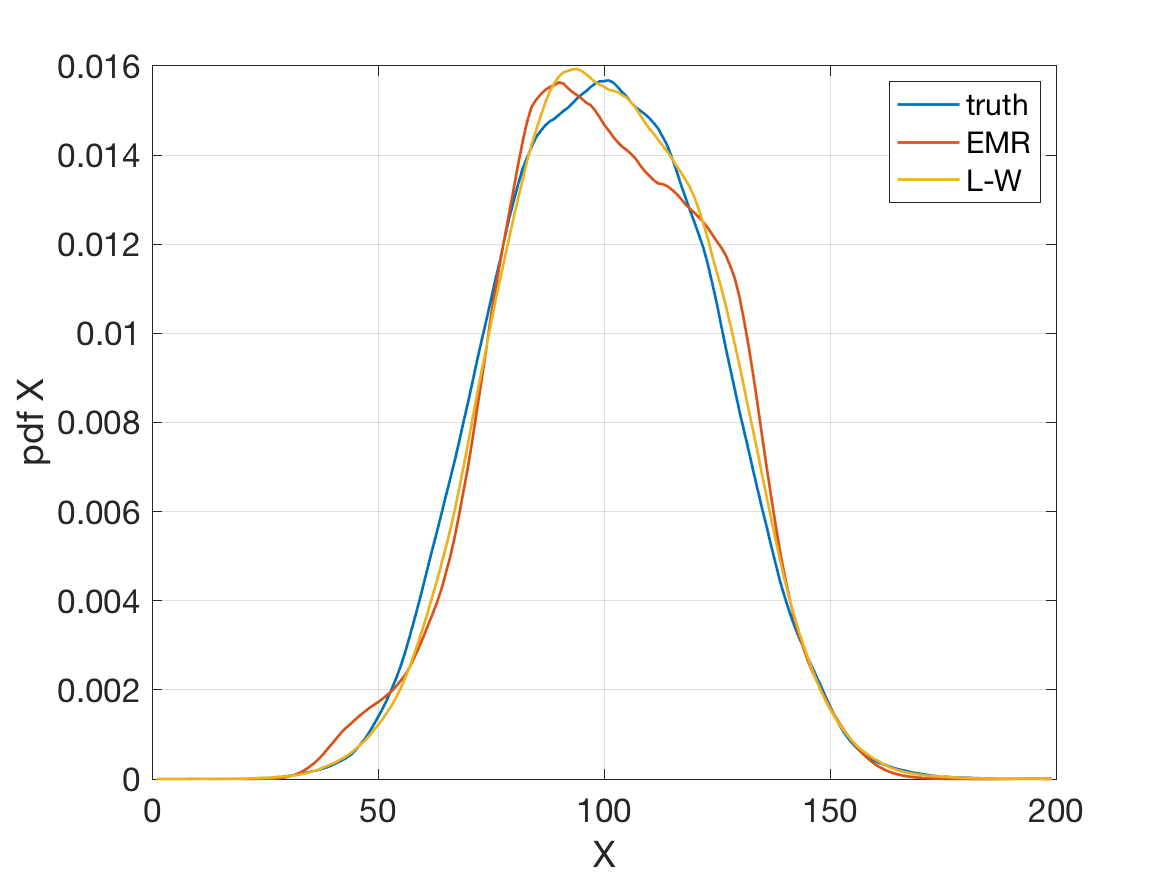
\includegraphics[width=\textwidth]{pdf_x_3.png}
%		%\caption{$y=x$}
%	\end{subfigure}
%	\hfill
%	\begin{subfigure}[b]{0.45\textwidth}
%		\centering
%		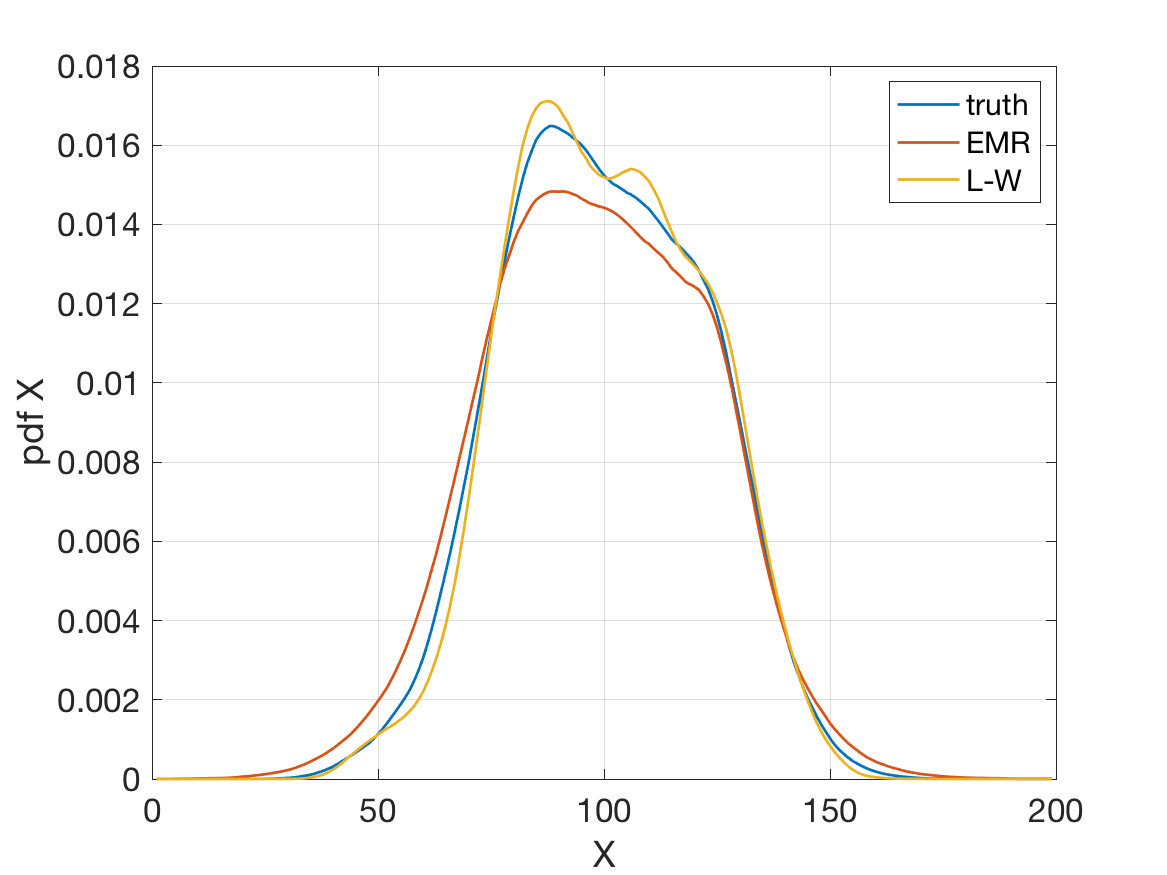
\includegraphics[width=\textwidth]{pdf_x_7.png}
%		%\caption{$y=3sinx$}
%	\end{subfigure}
%	\hfill
%	\caption{PDF's for the $X$-variable obtained using different methods indicated on the plots for $\tau =1 $ (left) and $\tau = 5$ (right).}
%\end{figure}
%
%
%
%\begin{figure}[H]
%	\centering
%	\begin{subfigure}[b]{0.3\textwidth}
%		\centering
%		\includegraphics[width=\textwidth]{error_x.png}
%		%\caption{$y=x$}
%	\end{subfigure}
%	\hfill
%	\begin{subfigure}[b]{0.3\textwidth}
%		\centering
%		\includegraphics[width=\textwidth]{error_y.png}
%		%\caption{$y=3sinx$}
%	\end{subfigure}
%	\hfill
%	\begin{subfigure}[b]{0.3\textwidth}
%		\centering
%		\includegraphics[width=\textwidth]{error_z.png}
%		%\caption{$y=5/x$}
%	\end{subfigure}
%	\caption{\label{errors} Absolute $L^2$-errors and standard deviations of the W-L parametrisation and EMR methodology with respect to the full model.}
%\end{figure}

\section*{Appendix C: the L84-L63 System}

On the previous appendix we investigated the ability of the empirical method to capture the features of the model by analysing time-series. The model was low dimensional and was fully observer in phase-space. Here, we shall repeat the same calculations in a dynamical system possesing a greater number of degrees of freedom, yet still low dimensional. 

The model we consider here is the result of coupling the L84 system \cite{Lorenz1984a} with the already mentioned L63. The model reads as
\begin{align}
dX&=-Y^2-Z^2-aX+a(F_0 + hx)\\
dY&=XY - bXZ - Y +G \\
dZ&=XZ+bXY-Z\\
dx&=\tau s (y-x)\\
dy&=\tau (\rho x - y -xz)\\
dz&=\tau (xy-\beta z)
\end{align}
With the parameter choice: $a=0.25,b=4,$ $F_0=8,$ $G=1,$ $s=10,$ $\rho = 28$ and $\beta =8/3$. The parameter $h$ measures the strength of the coupling and $\tau$ indicates the speed of the L63 system and ultimately, the time-scale difference.

The coupling of this model is one-way, in the sense that only the L63 system feeds into the L84 dynamics. This results (as noted in \cite{Vissio2018b}) in a fully Markovian parametrisation of the L63 variables. In this system, the correlation function that defines the stochastic noise $\eta(t)$ can be further expanded and simplified. Indeed, it can be written explicitly as:
\begin{equation}
C(\eta (0,\eta(t)))=\left \langle (x(0),0,0)\cdot (x(t),0,0) \right \rangle _{\mathrm{L63}}.
\end{equation}
Since L84 does not feed into L63, the evolution of $x(t)$ only obeys the dynamics of L63. Thus, the decorrelation of the noise scales like that of $x(t)$. 

In the numerical experiments, the bookkeeping parameters employed are $h=0.25$ and $\tau$ is indicated on the plots. The coupled, uncoupled and parametrised models were integrated for $7300$ time-units (corresponding to 100 years) with a time-step of $0.005$ time-units.


\subsection{EMR outputs}

Here we present a brief summary of the  outputs given by the EMR in the context of the coupled L84-L63 model. In this set of experiments partial observations of the system are taken, namely, only the output of the variables $X$, $Y$ and $Z$ are going to be saved. This provokes the introduction of noisy and memory terms as indicated earlier. The questions we seek to answer are:

\begin{enumerate}
	\item How well does the EMR procedure approximate the coefficients as a function of the coupling parameter $h$?
	\item How well does the EMR procedure approximate the coefficients as a function of the coupling parameter $h$?
	\item How does the memory/noise term given by the second level in the EMR behave as a function of $h$?
\end{enumerate}

\begin{figure}[H]
	\centering
	\begin{subfigure}[b]{0.3\textwidth}
		\centering
		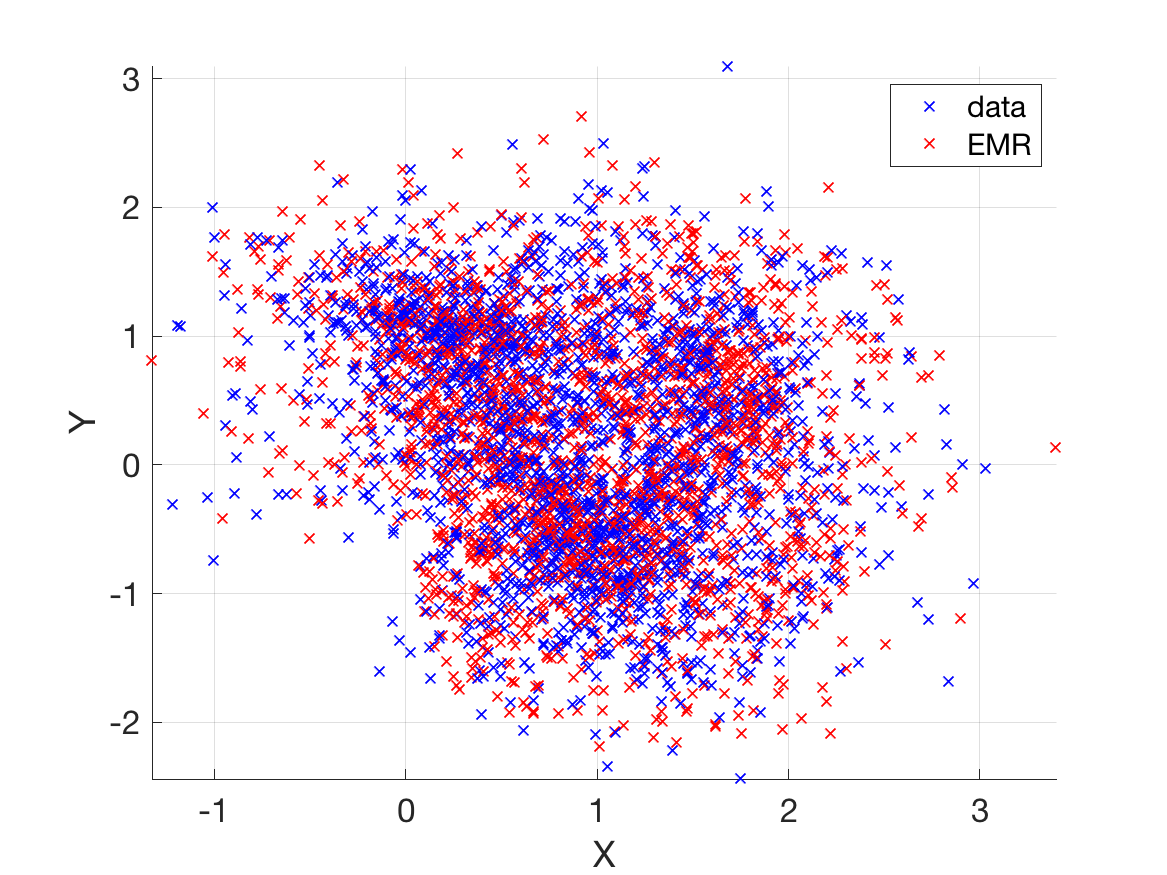
\includegraphics[width=\textwidth]{plots/l84l63/traj1l84.png}
		%\caption{$y=x$}
	\end{subfigure}
	\hfill
	\begin{subfigure}[b]{0.3\textwidth}
		\centering
		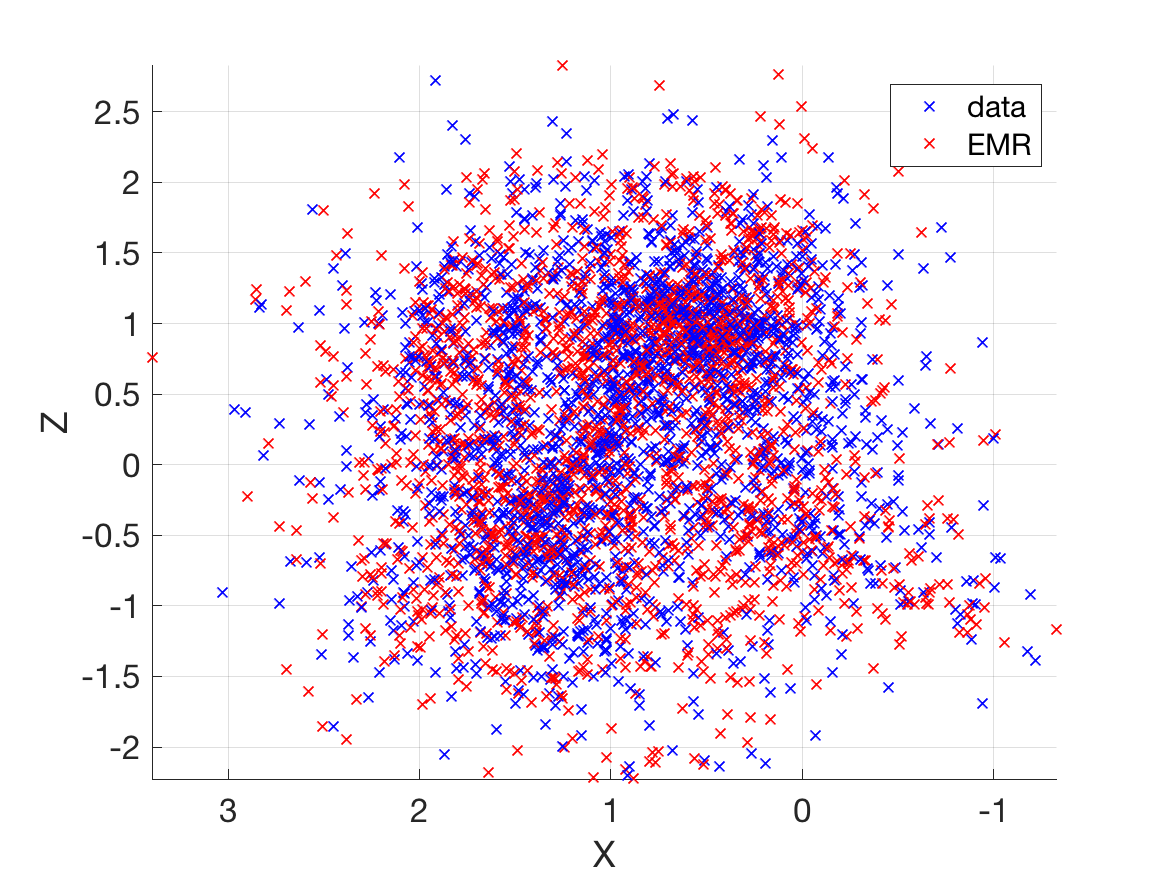
\includegraphics[width=\textwidth]{plots/l84l63/traj2l84.png}
		%\caption{$y=3sinx$}
	\end{subfigure}
	\hfill
	\begin{subfigure}[b]{0.3\textwidth}
		\centering
		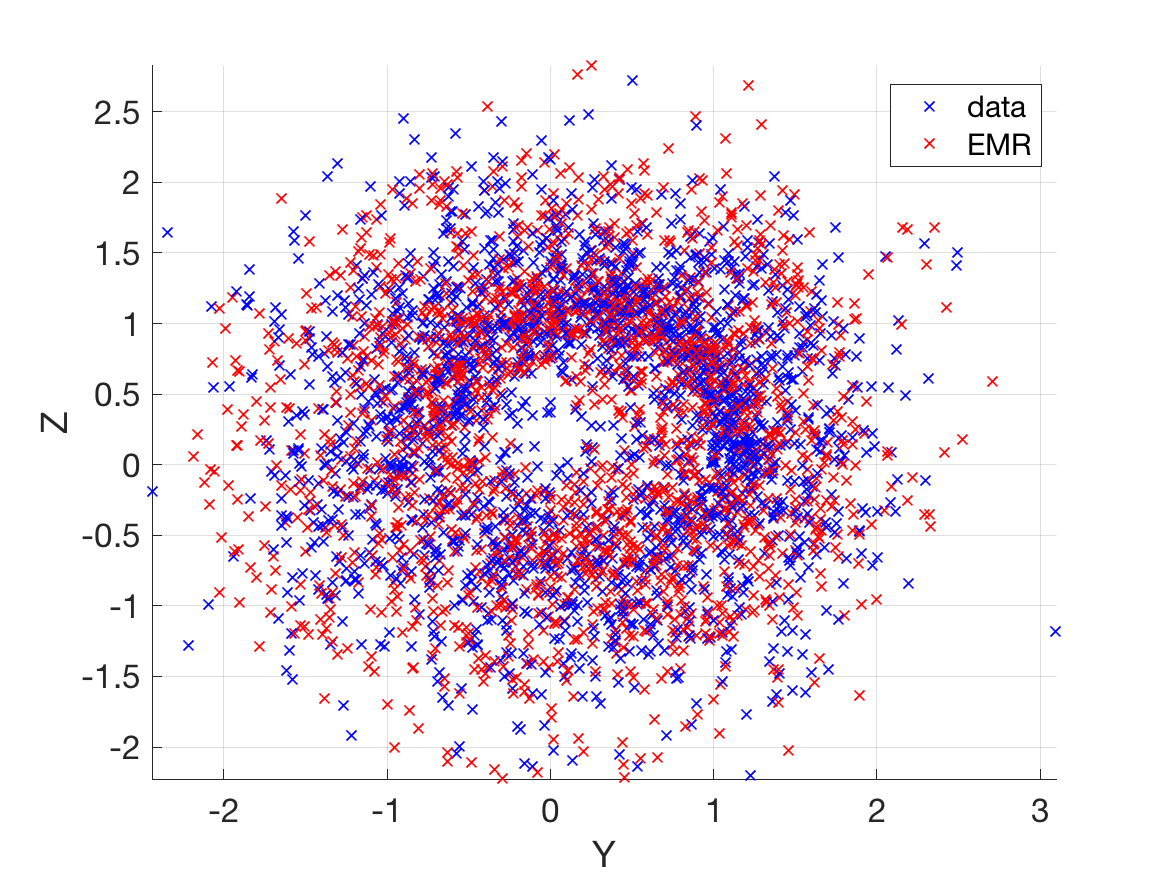
\includegraphics[width=\textwidth]{plots/l84l63/traj3l84.png}
		%\caption{$y=5/x$}
	\end{subfigure}
	\caption{Time-series of L84-L63 plotted on phase space ($h=0.25$).}
\end{figure}


\begin{figure}[H]
	\centering
	\begin{subfigure}[b]{0.3\textwidth}
		\centering
		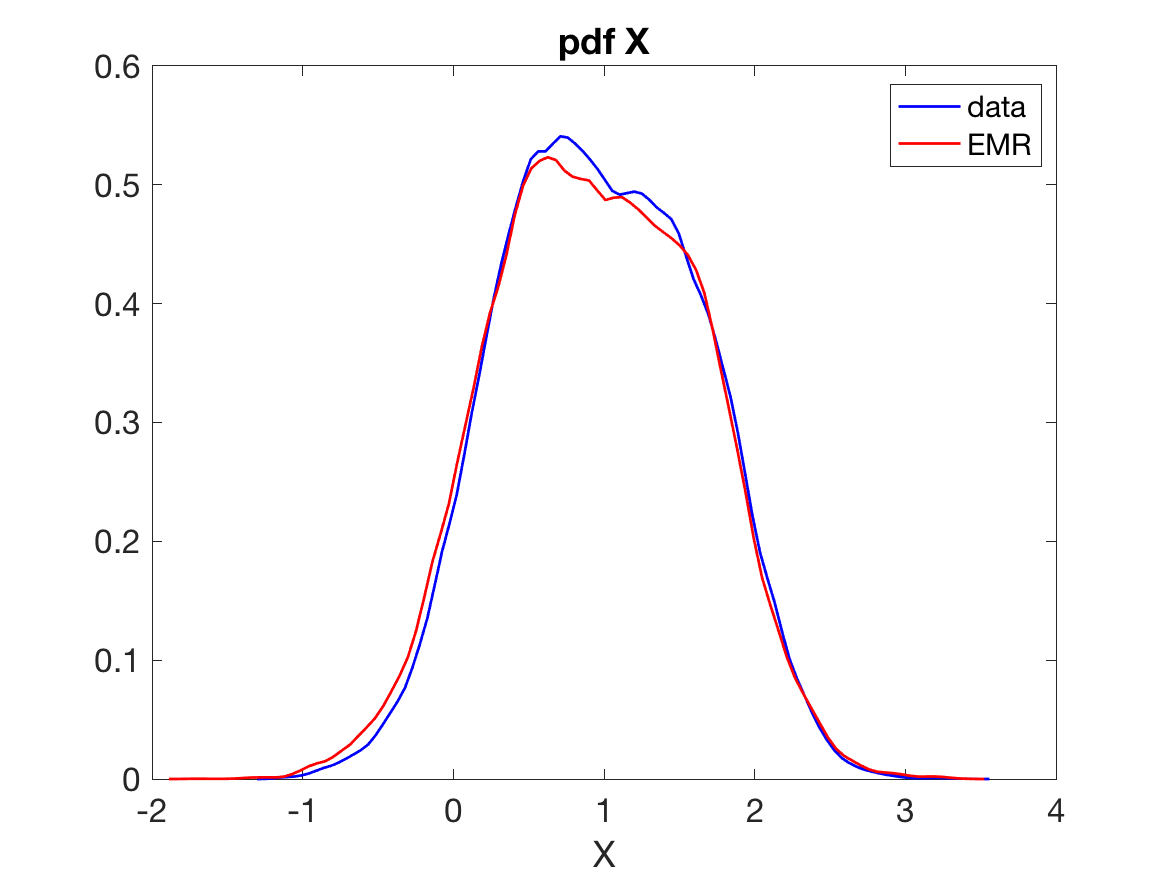
\includegraphics[width=\textwidth]{plots/l84l63/emrpdfxl84025.png}
		%\caption{$y=x$}
	\end{subfigure}
	\hfill
	\begin{subfigure}[b]{0.3\textwidth}
		\centering
		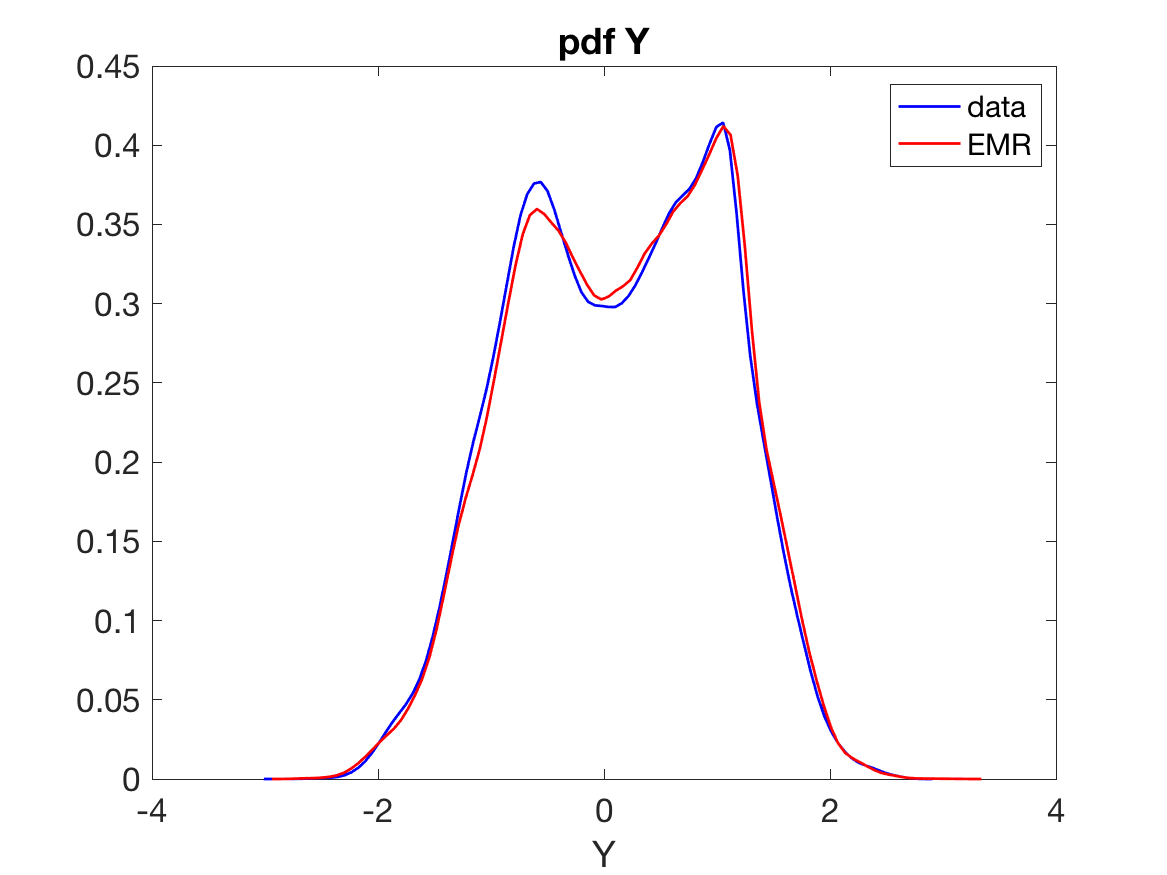
\includegraphics[width=\textwidth]{plots/l84l63/emrpdfyl84025.png}
		%\caption{$y=3sinx$}
	\end{subfigure}
	\hfill
	\begin{subfigure}[b]{0.3\textwidth}
		\centering
		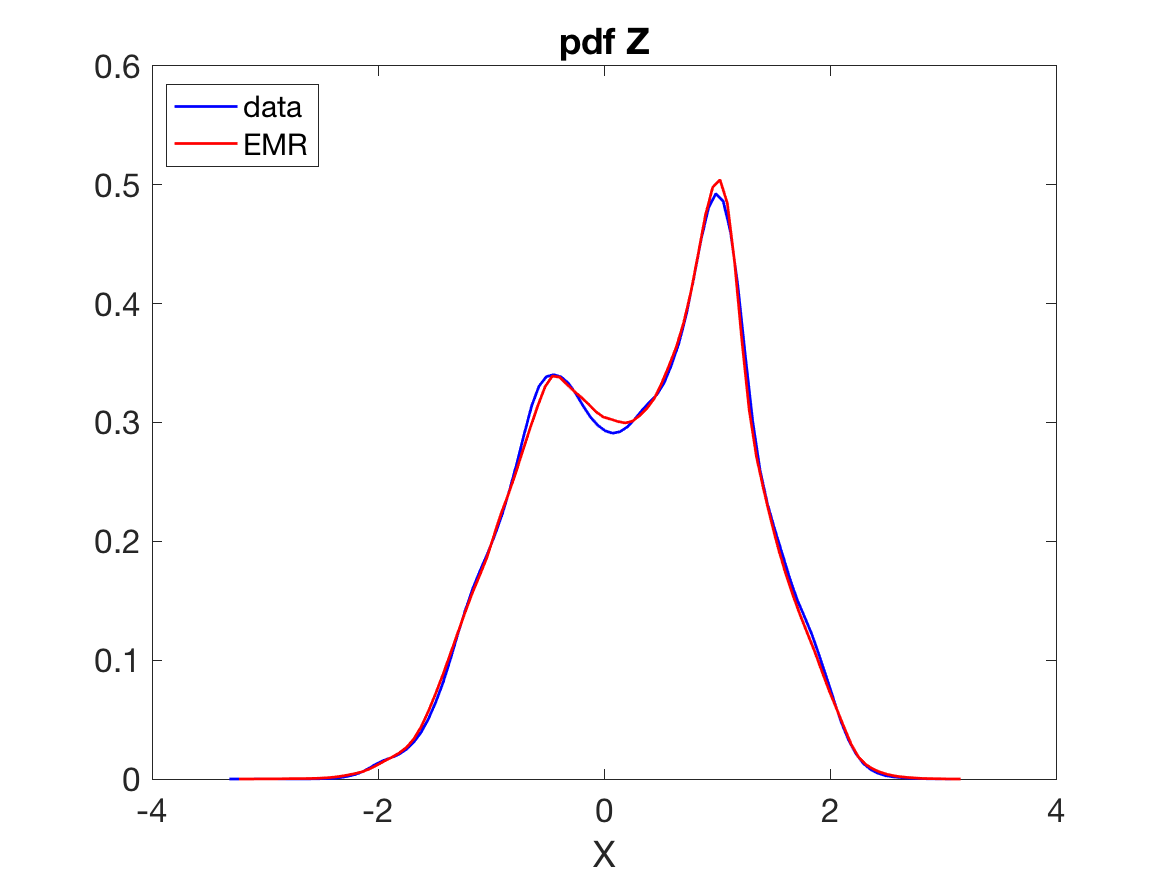
\includegraphics[width=\textwidth]{plots/l84l63/emrpdfzl84025.png}
		%\caption{$y=5/x$}
	\end{subfigure}
	\caption{PDF's of L84-L63 ($h=0.25$).}
\end{figure}

\begin{figure}[H]
	\centering
	\begin{subfigure}[b]{0.3\textwidth}
		\centering
		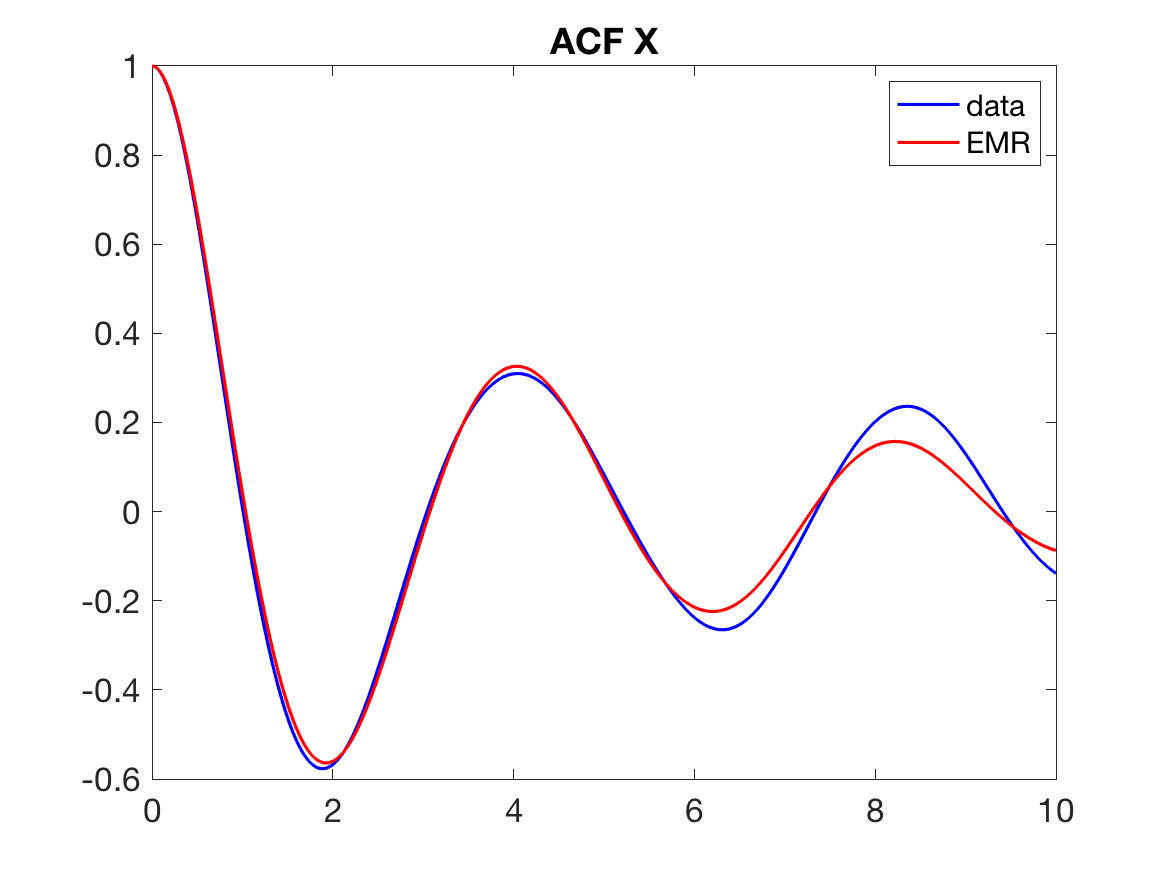
\includegraphics[width=\textwidth]{plots/l84l63/emracfxl84025.png}
		%\caption{$y=x$}
	\end{subfigure}
	\hfill
	\begin{subfigure}[b]{0.3\textwidth}
		\centering
		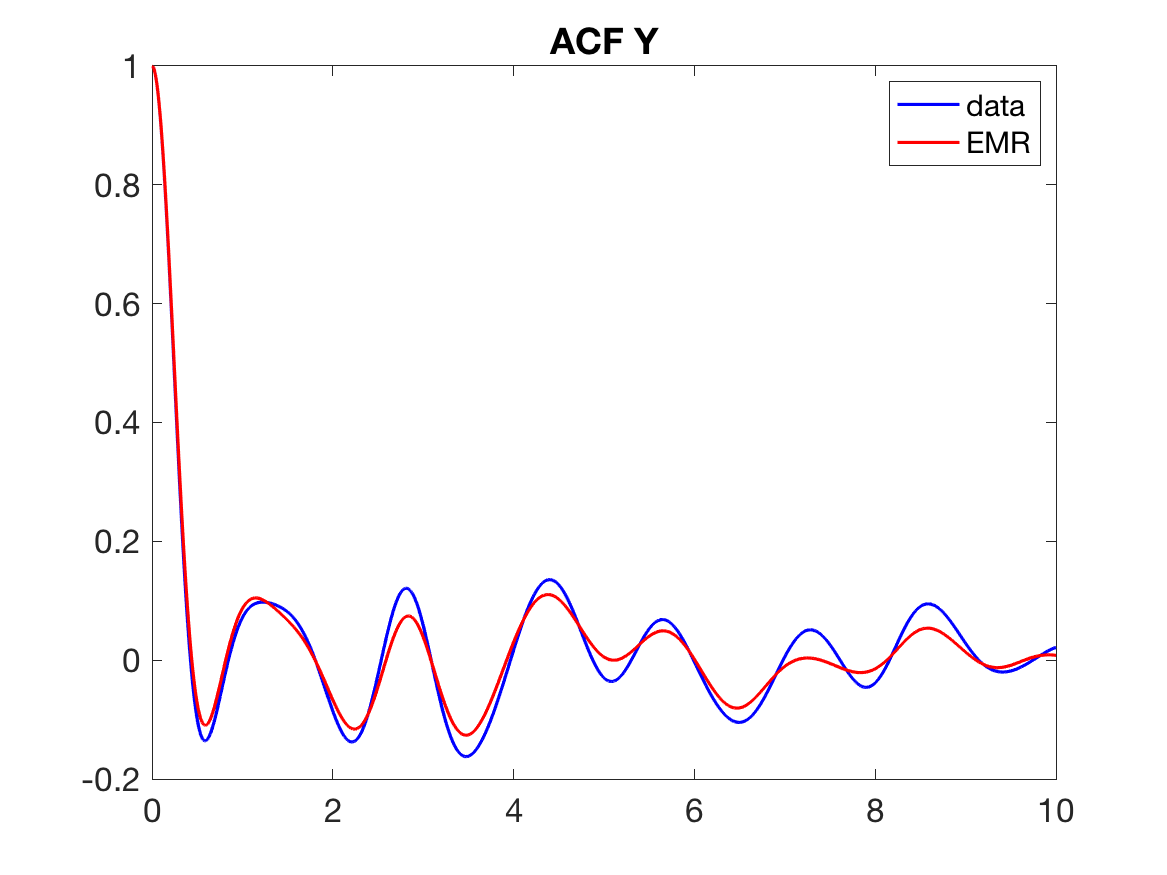
\includegraphics[width=\textwidth]{plots/l84l63/emracfyl84025.png}
		%\caption{$y=3sinx$}
	\end{subfigure}
	\hfill
	\begin{subfigure}[b]{0.3\textwidth}
		\centering
		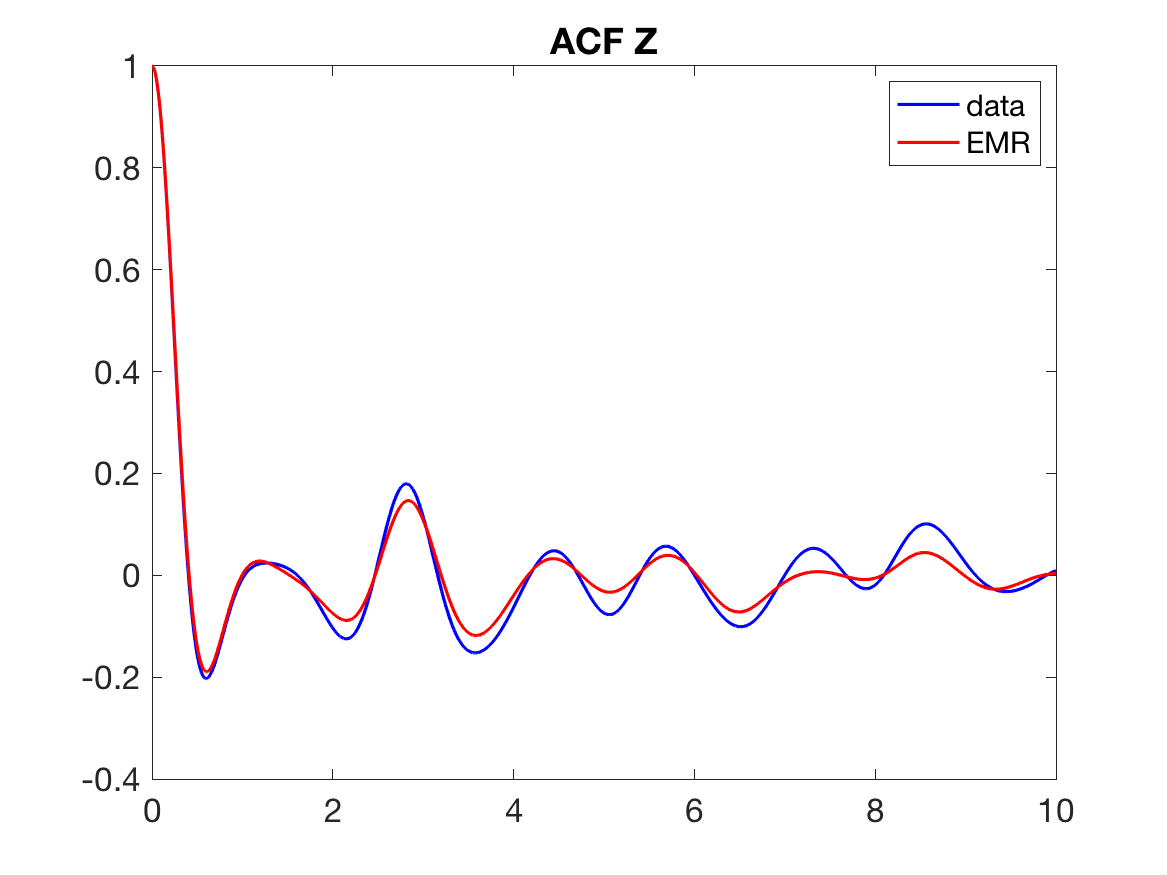
\includegraphics[width=\textwidth]{plots/l84l63/emracfzl84025.png}
		%\caption{$y=5/x$}
	\end{subfigure}
	\caption{Autocorrelation functions of L84-L63 ($h=0.25$).}
\end{figure}

\begin{figure}[H]
	\centering
	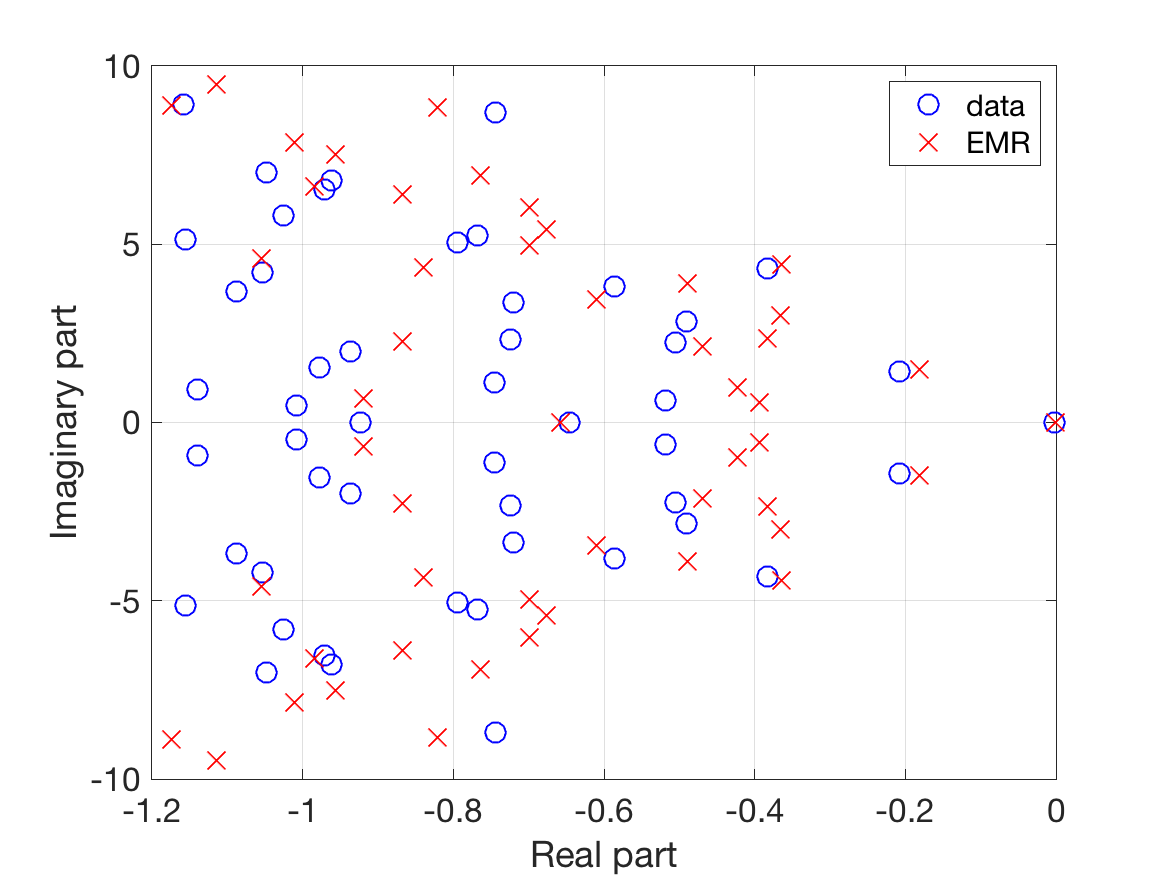
\includegraphics[width=\textwidth]{plots/l84l63/especl84.png}
	\caption{Observed ergodicity spectrum of L84-L63 ($h=0.25$).}
\end{figure}


\begin{figure}[H]
	\centering
	\begin{subfigure}[b]{0.3\textwidth}
		\centering
		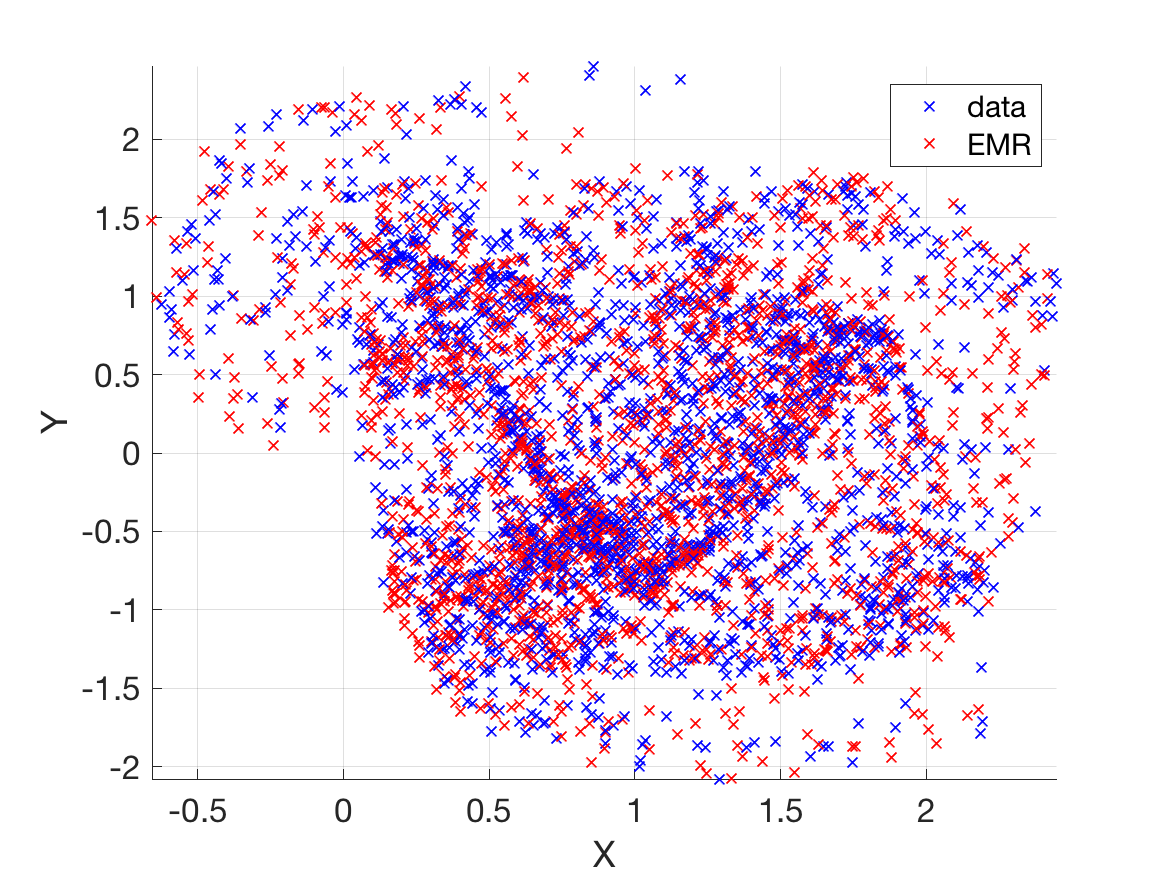
\includegraphics[width=\textwidth]{plots/l84l63/traj1l840025.png}
		%\caption{$y=x$}
	\end{subfigure}
	\hfill
	\begin{subfigure}[b]{0.3\textwidth}
		\centering
		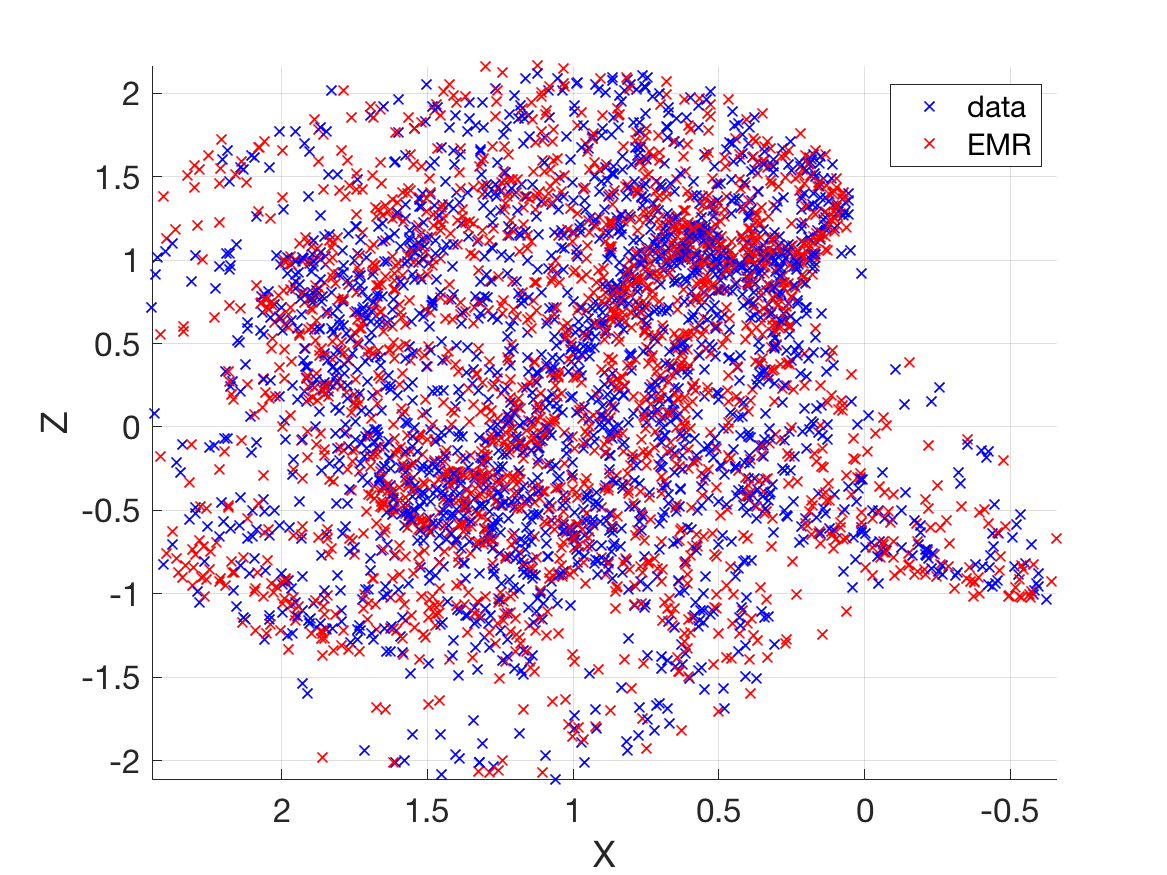
\includegraphics[width=\textwidth]{plots/l84l63/traj2l840025.png}
		%\caption{$y=3sinx$}
	\end{subfigure}
	\hfill
	\begin{subfigure}[b]{0.3\textwidth}
		\centering
		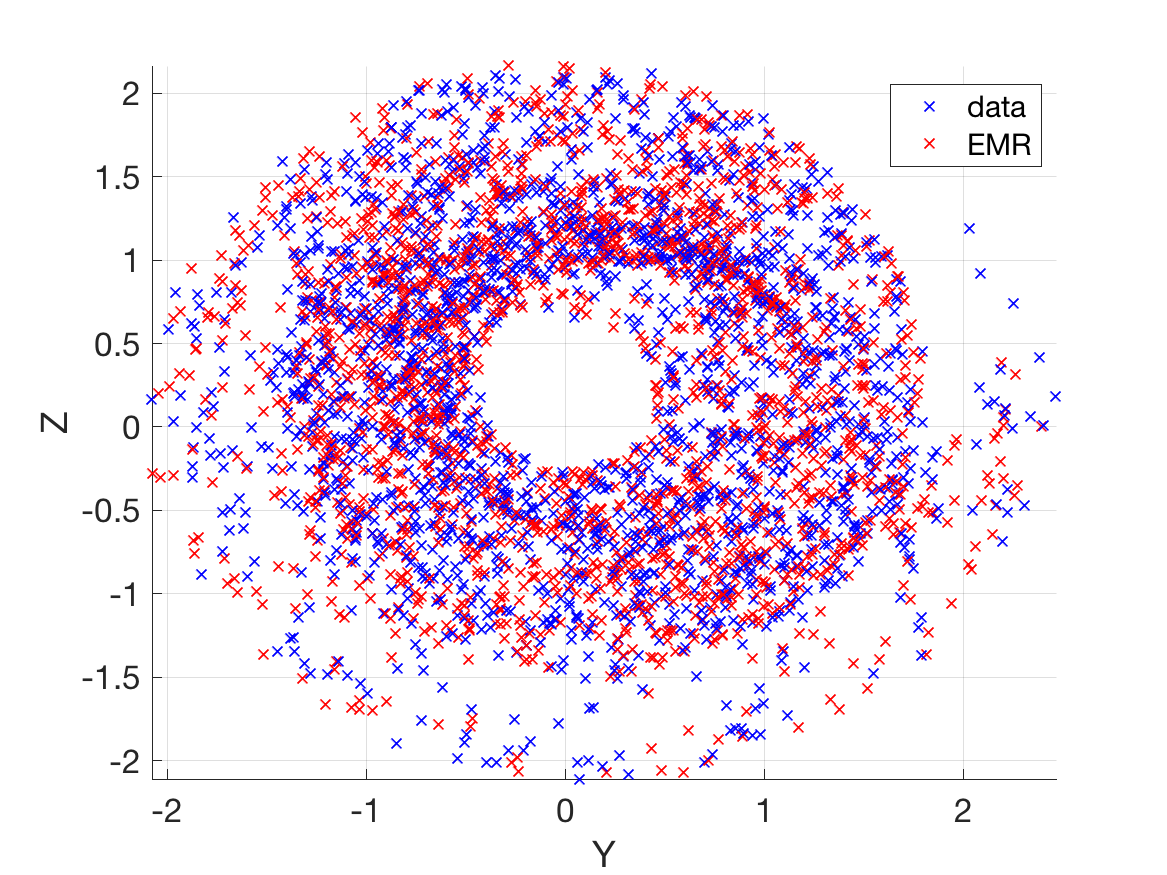
\includegraphics[width=\textwidth]{plots/l84l63/traj3l840025.png}
		%\caption{$y=5/x$}
	\end{subfigure}
	\caption{Time-series of L84-L63 plotted on phase space ($h=0.025$).}
\end{figure}


\begin{figure}[H]
	\centering
	\begin{subfigure}[b]{0.3\textwidth}
		\centering
		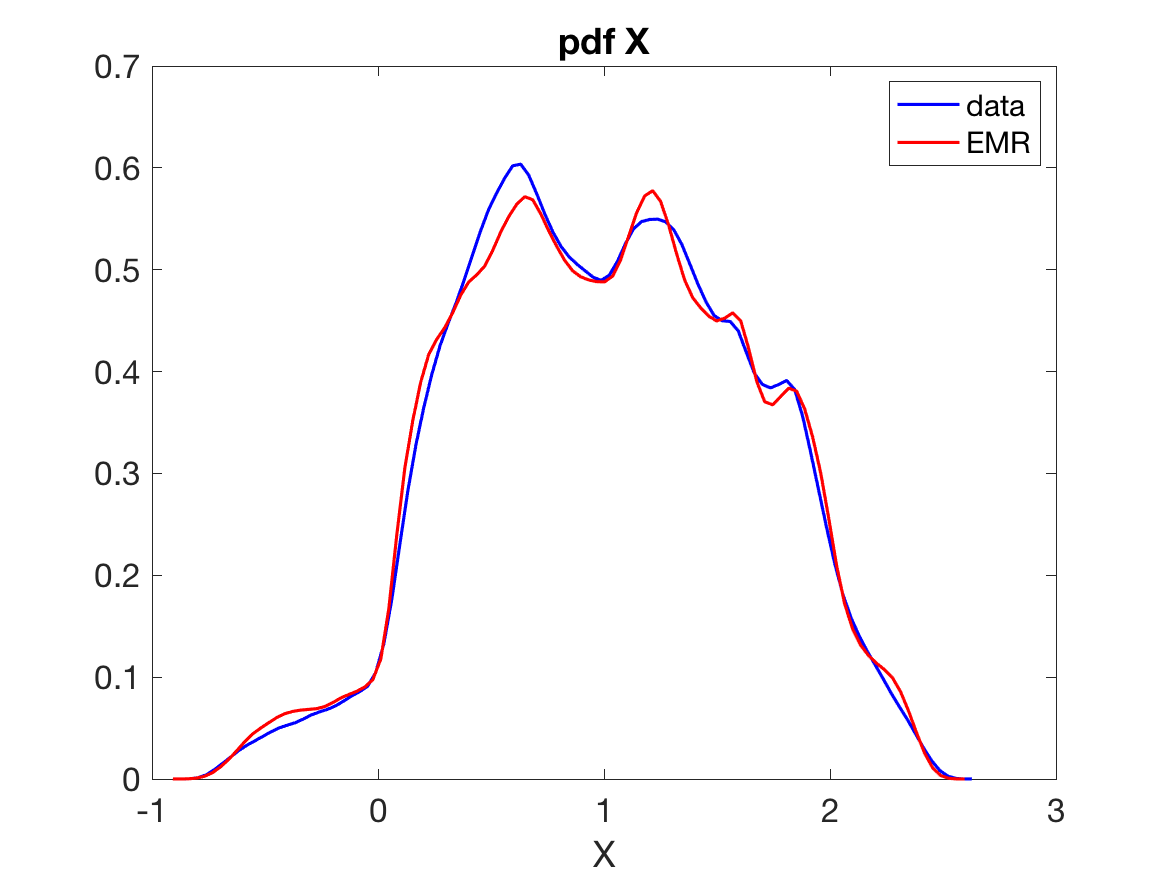
\includegraphics[width=\textwidth]{plots/l84l63/pdfxl840025.png}
		%\caption{$y=x$}
	\end{subfigure}
	\hfill
	\begin{subfigure}[b]{0.3\textwidth}
		\centering
		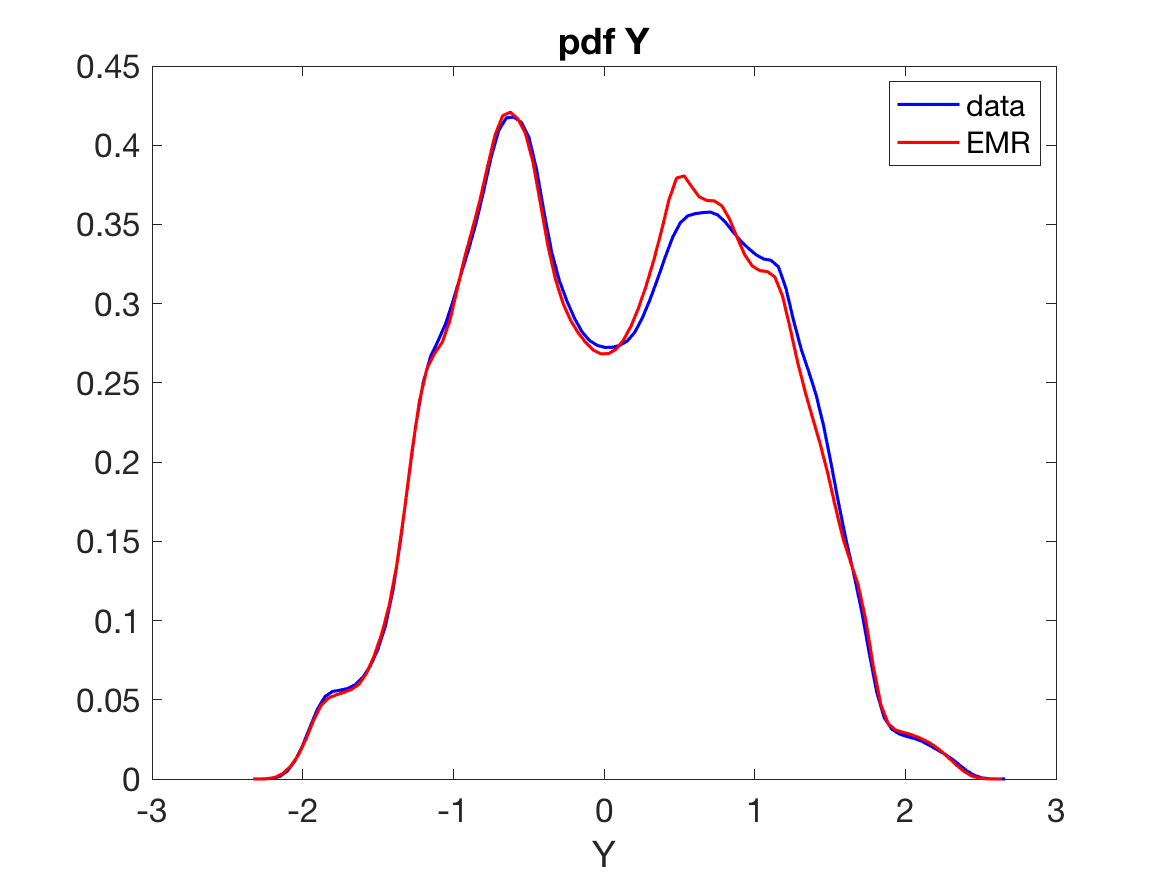
\includegraphics[width=\textwidth]{plots/l84l63/pdfyl840025.png}
		%\caption{$y=3sinx$}
	\end{subfigure}
	\hfill
	\begin{subfigure}[b]{0.3\textwidth}
		\centering
		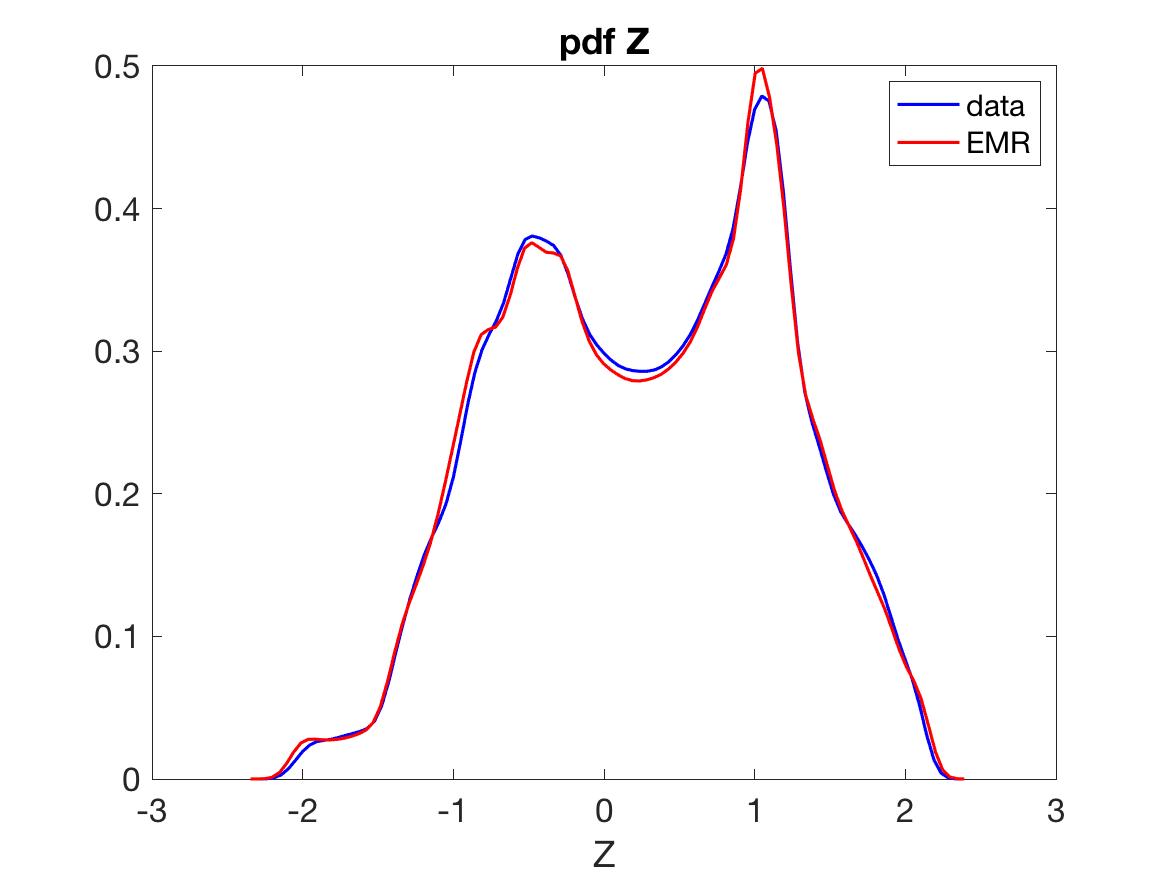
\includegraphics[width=\textwidth]{plots/l84l63/pdfzl840025.png}
		%\caption{$y=5/x$}
	\end{subfigure}
	\caption{PDF's of L84-L63 ($h=0.025$).}
\end{figure}

\begin{figure}[H]
	\centering
	\begin{subfigure}[b]{0.3\textwidth}
		\centering
		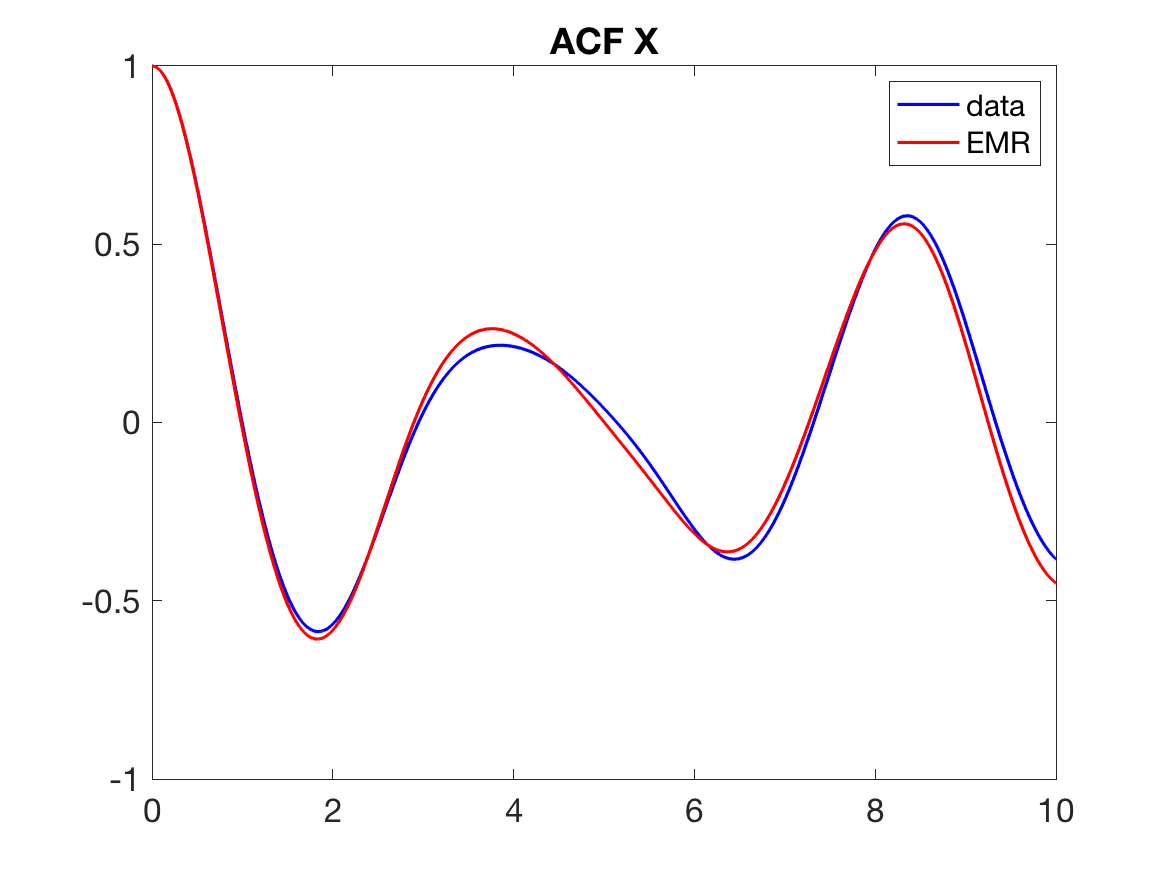
\includegraphics[width=\textwidth]{plots/l84l63/acfxl840025.png}
		%\caption{$y=x$}
	\end{subfigure}
	\hfill
	\begin{subfigure}[b]{0.3\textwidth}
		\centering
		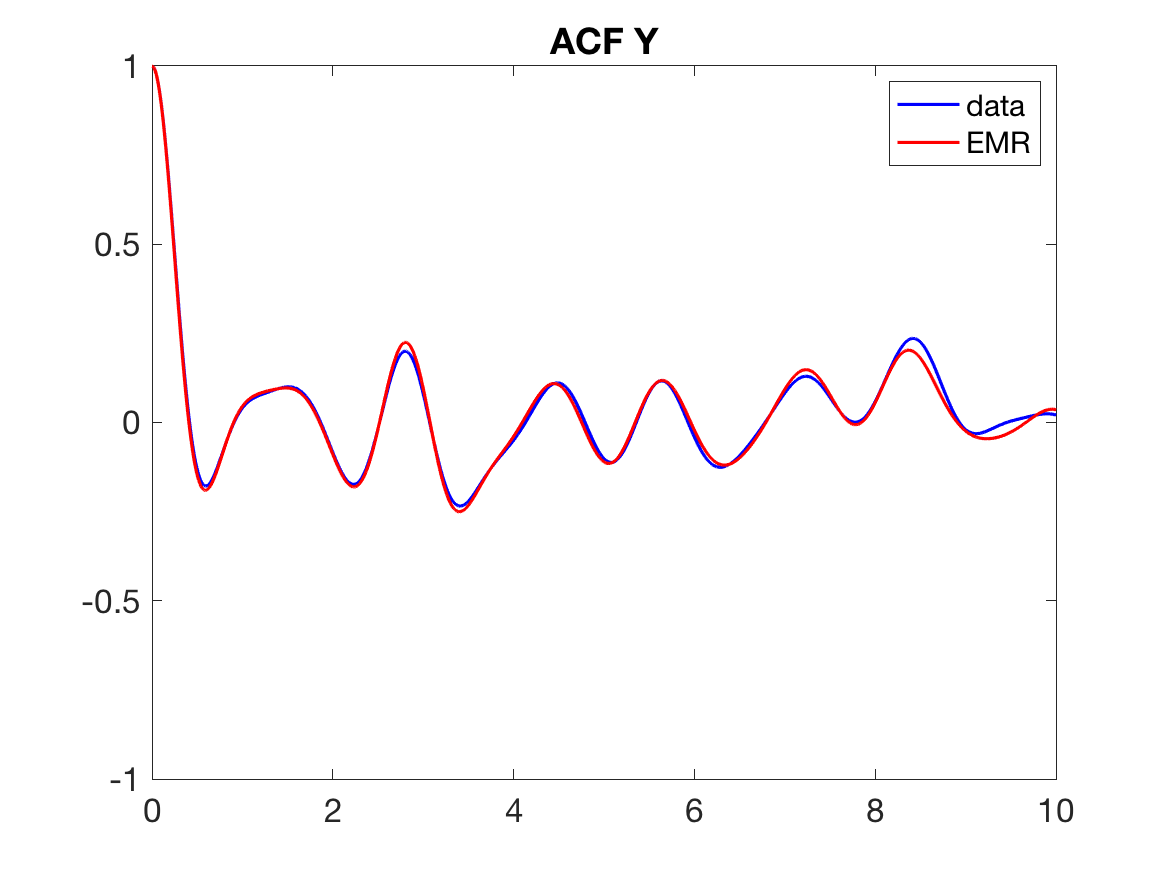
\includegraphics[width=\textwidth]{plots/l84l63/acfyl840025.png}
		%\caption{$y=3sinx$}
	\end{subfigure}
	\hfill
	\begin{subfigure}[b]{0.3\textwidth}
		\centering
		\includegraphics[width=\textwidth]{plots/l84l63/acfzl840025.png}
		%\caption{$y=5/x$}
	\end{subfigure}
	\caption{Autocorrelation functions of L84-L63 ($h=0.025$).}
\end{figure}

\begin{figure}[H]
	\centering
	\includegraphics[width=\textwidth]{plots/l84l63/especl840025.png}
	\caption{Observed ergodicity spectrum of L84-L63 ($h=0.025$).}
\end{figure}

\subsection{Convergence}

Convergence in the EMR approach is determined by the level of stochasticity that the residual of the last level has, as explained on the main text. On Fig.~\ref{convergence emr} we plotted the mean of the determination coefficients of each dimension and we show that convergence in the EMR approach depends mildly on the coupling parameter. Indeed, for $h=0.25$ we observe that around 18 levels are necessary before achieving the optimal level, whereas for $h=0.025$ convergence is attained with 15 levels. This agrees with what one would initially expect. Further, the addition of additive white noise in the L63 system can in fact accelerate the convergence of the method, as seen in Figure \ref{convergence with noise}.

\begin{figure}[H]
	\centering
	\begin{subfigure}[b]{0.49\textwidth}
		\centering
		\includegraphics[width=\textwidth]{plots/l84l63/emr_diagnostic_025.png}
		%\caption{$y=x$}
	\end{subfigure}
	\hfill
	\begin{subfigure}[b]{0.49\textwidth}
		\centering
		\includegraphics[width=\textwidth]{plots/l84l63/emr_diagnostic_0025.png}
		%\caption{$y=3sinx$}
	\end{subfigure}
	\caption{\label{convergence emr}Determination coefficient of the EMR method as a function of number of levels ($h=0.25$ on the left and $0.025$ on the right).}
\end{figure}




\begin{figure}[H]
	\centering
	\includegraphics[width=\textwidth]{plots/l84l63/emr_diagnostics_noise.png}
	\caption{\label{convergence with noise}EMR diagnostics in the noisy L84-L63 system ($h=0.25$ and $\sigma = 1.5$).}
\end{figure}


\subsection{Model Coefficients and Memory Terms}

\begin{table}[H]
	\centering
	\begin{tabular}{c | cccccccccc}
		EMR & $1$ & $x$ & $y$ & $z$ & $x^2$ & $xy$ & $y^2$ & $xz$ & $yz$ & $z^2$  \\ \hline
		$f_X$ & \hphantom{-}1.80 & -0.13 & \hphantom{-}0.02 & \hphantom{-}0.00 & \hphantom{-}0.00 & -0.02 & -0.95 & -0.00 & -0.00 & -0.95\\
		$f_Y$ & \hphantom{-}0.97& \hphantom{-}0.04 & -0.98 & \hphantom{-}0.02 & -0.01 & \hphantom{-}0.92 & \hphantom{-}0.00& -4.02 & \hphantom{-}0.00 & \hphantom{-}0.01 \\ 
		$f_Z$ & \hphantom{-}0.03 & -0.02 & -0.02& -0.98 &\hphantom{-}0.01& \hphantom{-}4.02 & \hphantom{-}0.00 & \hphantom{-}0.92 & -0.01 & \hphantom{-}0.00 \\ 
	\end{tabular}
	\caption{Means of the coefficients of L84-L63 estimated on an ensemble of 20 runs for $h=0.25$. The standard deviations are not shown since the results were very robust.}
\end{table}

\begin{table}[H]
	\centering
	\begin{tabular}{c | ccccccc}
		EMR & $1$ & $x$ & $y$ & $z$ & $r_1$ & $r_2$ & $r_3$  \\ \hline
		$f^{(1)}_X$ & 0.00& 0.00 & 0.00 & 0.00 & -0.08& 0.12 & 1.2 \\ 
		$f^{(1)}_Y$ & 0.00 & 0.00 & 0.00 & 0.00 & 0.02 & 0.03 & -3.78 \\ 
		$f^{(1)}_Z$ & 0.00 & 0.00 & 0.00 & 0.00 & 0.01 & 3.64 & -0.37  \\ 
	\end{tabular}
	\caption{Means of the coefficients for the second level of L84-L63 estimated on an ensemble of 20 runs for $h=0.25$. The standard deviations are not shown since the results were very robust.}
\end{table}

\begin{table}[H]
	\centering
	\begin{tabular}{c | cccccccccc}
		EMR & $1$ & $x$ & $y$ & $z$ & $x^2$ & $xy$ & $y^2$ & $xz$ & $yz$ & $z^2$  \\ \hline
		$f_X$ & 2.00 & -0.26& 0.00 & 0.00 & 0.00 & 0.00 & -1 & 0.00 & 0.00 & -1 \\
		$f_Y$ & 0.97 & 0.05 & -0.97 & 0.02 & -0.02 & 0.92 & 0.00 & -4.02& 0.00 & 0.01 \\
		$f_Z$ & 0.02& -0.03 & -0.023 & -0.97 & 0.02 & 4.02 & 0.00 & 0.92 & 0.00 & 0.00 \\ 
	\end{tabular}
	\caption{Means of the coefficients of L84-L63 estimated on an ensemble of 20 runs for $h=0.025$. The standard deviations are not shown since the results were very robust.}
\end{table}

\begin{table}[H]
	\centering
	\begin{tabular}{c | ccccccc}
		EMR & $1$ & $x$ & $y$ & $z$ & $r_1$ & $r_2$ & $r_3$  \\ \hline
		$f^{(1)}_X$ & 0.00 & 0.00 & 0.00 & 0.00 & -0.07 & 0.02 & 0.20 \\ 
		$f^{(1)}_Y$ & 0.00& 0.00 & 0.00 &0.00& 0.00 & 0.23 & -3.08 \\ 
		$f^{(1)}_Z$ & 0.00 & 0.00 & 0.00 & 0.00 & 0.00 & 3.55 & -0.47 \\ 
	\end{tabular}
	\caption{Means of the coefficients for the second level of L84-L63 estimated on an ensemble of 20 runs for $h=0.025$. The standard deviations are not shown since the results were very robust.}
\end{table}

\subsection{Residuals}

The novelty introduced by the EMR approach is that the errors produced by the nonlinear regression at the first level are coupled to the stochastic correction, as explained earlier, in a linear fashion. It is of interest to understand how the residual is modelled and how it compares to the stochastic correction predicted by the WL parametrisation.

The question now is: does the residual emulated by the EMR resemble the statistical properties of that predicted by WL? Indeed, on Fig.~\ref{residuals} we plotted the residuals and stochastic corrections obtained using the methodologies indicated. Regarding the statistical properties of such residuals, that is illustrated on Fig.~\ref{ergodicity spectrum}, where the leading resonances indicate the rate at which variables decorrelate. As we can see, the leading resonances of the residual simulated by the EMR match perfectly that of the stochastic noise obtained for the WL parametrisation.


\begin{figure}[H]
	\centering
	\begin{subfigure}[b]{0.49\textwidth}
		\centering
		\includegraphics[width=\textwidth]{plots/l84l63/emr_residuals_1.png}
		%\caption{$y=x$}
	\end{subfigure}
	\hfill
	\begin{subfigure}[b]{0.49\textwidth}
		\centering
		\includegraphics[width=\textwidth]{plots/l84l63/lw_stochastic_term.png}
		%\caption{$y=3sinx$}
	\end{subfigure}
	\hfill
	\begin{subfigure}[b]{0.49\textwidth}
		\centering
		\includegraphics[width=\textwidth]{plots/l84l63/emr_residuals_sim.png}
		%\caption{$y=3sinx$}
	\end{subfigure}
	\hfill
	\begin{subfigure}[b]{0.49\textwidth}
		\centering
		\includegraphics[width=\textwidth]{plots/l84l63/xl63.png}
		%\caption{$y=3sinx$}
	\end{subfigure}
	\caption{\label{residuals} Residuals and stochastic noise of the different methods. The top-left figure shows the residual of the first level of the EMR model. The top-right figure shows a run of a red noise with the correlation properties predictedby the WL parametrisation. The bottom-left plot shows a run of the residual of the EMR model (it is decoupled from the main level) and the bottom right shows the $x$-variable of the L63 model.}
\end{figure}

\begin{figure}[H]
	\centering
	\begin{subfigure}[b]{0.32\textwidth}
		\centering
		\includegraphics[width=\textwidth]{plots/l84l63/ergodicity_spectrum_residuals.png}
		%\caption{$y=x$}
	\end{subfigure}
	\hfill
	\begin{subfigure}[b]{0.32\textwidth}
		\centering
		\includegraphics[width=\textwidth]{plots/l84l63/ergodicity_rates_residuals.png}
		%\caption{$y=3sinx$}
	\end{subfigure}
	\hfill
	\begin{subfigure}[b]{0.32\textwidth}
		\centering
		\includegraphics[width=\textwidth]{plots/l84l63/acf_residuals.png}
		%\caption{$y=3sinx$}
	\end{subfigure}
	\caption{\label{ergodicity spectrum} Observed ergodicity spectrum and autocorrelation functions of the different parametrisations.}
\end{figure}

\begin{figure}[H]
	\centering
	\begin{subfigure}[b]{0.49\textwidth}
		\centering
		\includegraphics[width=\textwidth]{plots/l84l63/acf_res_t5.png}
		%\caption{$y=3sinx$}
	\end{subfigure}
	\hfill
	\begin{subfigure}[b]{0.49\textwidth}
		\centering
		\includegraphics[width=\textwidth]{plots/l84l63/acf_res_t1.png}
		%\caption{$y=3sinx$}
	\end{subfigure}
	\caption{\label{decorrelation residuals} Decorrelation of residuals of the EMR methodology and of stochastic noise induced by the WL parametrisation for different coupling strengths. We show two cases where the time-scale separation is: $\tau = 1$ (right) and $\tau = 5$.}
\end{figure}

\subsection{Comparison}

The target of the parametrisations presented here is to be able to reproduce the climatology of the system without needing to integrate of the full dynamics. Measuring differences in the climatology boils down to measuring differences between the attractors and invariant measures of the different models. For simplicity we shall take the Kolmogorov-Smirnov statistic of the projected invariant measures of the system onto the main coordinates $X$, $Y$ and $Z$. To attribute a score to the methodologies we calculate the Kolmogorov-Smirnov statistics of the obtained climatologies with respect to the data coming from the whole model. The Kolmogorov-Smirnov statistic does not measure distances in a strict sense. Hence, the Wasserstein distance \cite{villani} is precisely defined for this purpose and has been suggested as a skill-measuring tool in the context of dynamical systems and climatology \cite{robin2017, Vissio2018b}. 

To assess the performances of the different methods, we ran ten integrations of the dynamics initialised with random intial conditions and applying a spinup of 10 years. The model was integrated for 100 years with a time-step of 0.005 time-units.
\begin{table}[H]
	\centering
	\begin{tabular}{l | ccc}
		& Data & EMR  & WL \\ 
		\hline 
		$\bar{X}$&$91.6 \pm 0.4$ &$ 94.7 \pm 0.5 $&$ 93.1 \pm 0.4 $\\ 
		$\bar{Y}$&$21.7 \pm 0.7 $&$ 15.1 \pm 1 $&$ 18.7 \pm 0.6 $\\ 
		$\bar{Z}$&$29.2 \pm 0.5 $& $26.4 \pm 0.3 $& $29.3 \pm 0.8 $\\ 
		$\mathrm{var}(X)$&$48.6 \pm 0.8 $& $50.2 \pm 1.7 $& $49.7 \pm 0.8$ \\ 
		$\mathrm{var}(Y)$&$84.7 \pm 0.5 $&$ 84.9 \pm 0.4$ &$ 83.8 \pm 1.9 $\\ 
		$\mathrm{var}(Z)$&$79.3 \pm 0.5 $& $82.6 \pm 0.4 $&$ 80.1 \pm 1.7$ \\ 
		$\mathrm{cov}(XY)$&$-17.6 \pm 0.6 $& $-13 \pm 0.8 $& $-15.3 \pm 0.4$ \\ 
		$\mathrm{cov}(XZ)$&$-6.6 \pm 0.4 $&$ -3.5 \pm 0.4 $& $-6.4 \pm 0.8$ \\ 
		$\mathrm{cov}(YZ)$&$0.3 \pm 0.4 $& $-2.7 \pm 0.2$ & $-0.2 \pm 0.6$ \\ 
	\end{tabular}
	\caption{\label{tablemoments1}Expectation value of the first two moments of the variables $X,Y$ and $Z$ from the L84-L63 model for the time-scale separation of $\tau = 1$ and coupling parameter $h=0.25$. The results are multiplied times $10^2$.}
\end{table}

\begin{table}[H]
	\centering
	\begin{tabular}{l | ccc}
		& Data & EMR  & WL \\ 
		\hline 
		$\bar{X}$&$97 \pm 0.4$ & $93.3 \pm 0.6 $& $97.8 \pm 0.4$ \\ 
		$\bar{Y}$&$14.2 \pm 0.8$ &$ 18.2 \pm 0.9$ &$ 12.9 \pm 0.8$ \\ 
		$\bar{Z}$&$30.9 \pm 0.4 $ &$ 28.4 \pm 0.6$ &$ 30.9 \pm 0.6$ \\ 
		$\mathrm{var}(X)$&$43.6 \pm 1.1$ &$ 52.2 \pm 0.5$ &$ 42.9 \pm 1$ \\ 
		$\mathrm{var}(Y)$&$82.8 \pm 0.2$ &$ 83.7 \pm 0.4 $& $83 \pm 0.9$ \\ 
		$\mathrm{var}(Z)$&$81.4 \pm 0.4 $& $81.4 \pm 0.4 $&$ 82.1 \pm 1.2 $\\ 
		$\mathrm{cov}(XY)$&$-11.5 \pm 0.6$ & $-15.1 \pm 0.7$ & $-10.5 \pm 0.7 $\\ 
		$\mathrm{cov}(XZ)$&$-7.9 \pm 0.4$ &$ -5.6 \pm 0.5$ &$ -7.9 \pm 0.6 $\\ 
		$\mathrm{cov}(YZ)$&$-1.5 \pm 0.3 $&$ -0.2 \pm 0.4 $& $-1.9 \pm 0.3 $\\ 
	\end{tabular}
	\caption{\label{tablemoments2}Expectation value of the first two moments of the variables $X,Y$ and $Z$ from the L84-L63 model for the time-scale separation of $\tau = 5$ and coupling parameter $h=0.25$. The results are multiplied times $10^2$.}
\end{table}

\begin{figure}[H]
	\centering
	\begin{subfigure}[b]{0.3\textwidth}
		\centering
		\includegraphics[width=\textwidth]{plots/l84l63/pdfxl84025.png}
		%\caption{$y=x$}
	\end{subfigure}
	\hfill
	\begin{subfigure}[b]{0.3\textwidth}
		\centering
		\includegraphics[width=\textwidth]{plots/l84l63/pdfyl84025.png}
		%\caption{$y=3sinx$}
	\end{subfigure}
	\begin{subfigure}[b]{0.3\textwidth}
		\centering
		\includegraphics[width=\textwidth]{plots/l84l63/pdfzl84025.png}
		%\caption{$y=3sinx$}
	\end{subfigure}
	\hfill
	\caption{PDFs of the variables of L84-L63 obtained using different methodologies. In this plot, the coupling parameter is $h=0.25$ and the scales separation $\tau = 5$.}
\end{figure}

\begin{figure}[H]
	\centering
	\begin{subfigure}[b]{0.3\textwidth}
		\centering
		\includegraphics[width=\textwidth]{plots/l84l63/acfxl84025.png}
		%\caption{$y=x$}
	\end{subfigure}
	\hfill
	\begin{subfigure}[b]{0.3\textwidth}
		\centering
		\includegraphics[width=\textwidth]{plots/l84l63/acfyl84025.png}
		%\caption{$y=3sinx$}
	\end{subfigure}
	\begin{subfigure}[b]{0.3\textwidth}
		\centering
		\includegraphics[width=\textwidth]{plots/l84l63/acfzl84025.png}
		%\caption{$y=3sinx$}
	\end{subfigure}
	\hfill
	\caption{ACFs of the variables of L84-L63 obtained using different methodologies. In this plot, the coupling parameter is $h=0.25$ and the scales separation $\tau = 5$.}
\end{figure}


\subsection{Non-trivial mean field forcing}

In the case presented earlier, the mean field contribution to the WL parametrisation was trivial, due to the symmetry of the $x$-variable in the L63 system. Here, we shall consider a perturbation that leads to non-trivial mean field correction term. This is simply attained by replacing the $x$ forcing by $z$, which has a non-zero mean in the L63 system. This change has two implications. Since the steady state mean value of the forcing is non-zero, the addition of such mean into the dynamic should provide a first order approximation to the statistics of the coupled model. Secondly, the variable $z$ decorrelates very slowly in the L63 system. Therefore, we will test what the effects of this is when empirically approximating the model using the EMR methodology.

\begin{figure}[H]
	\centering
	\includegraphics[width=0.5\textwidth]{plots/l84l63/emr_diagnostic_025z.png}
	\hfill
	\caption{Determination coefficient of the EMR method in the modified L84-L63 model as a function of number of levels ($h=0.25$).}
\end{figure}

\begin{figure}[H]
	\centering
	\begin{subfigure}[b]{0.3\textwidth}
		\centering
		\includegraphics[width=\textwidth]{plots/l84l63/pdfx025z.png}
		%\caption{$y=x$}
	\end{subfigure}
	\begin{subfigure}[b]{0.3\textwidth}
		\centering
		\includegraphics[width=\textwidth]{plots/l84l63/pdfy025z.png}
		%\caption{$y=3sinx$}
	\end{subfigure}
	\begin{subfigure}[b]{0.3\textwidth}
		\centering
		\includegraphics[width=\textwidth]{plots/l84l63/pdfz025z.png}
		%\caption{$y=3sinx$}
	\end{subfigure}
	\hfill
	\caption{PDF's of the observed variables $X,Y,Z$ obtained using full-model integrations and parametrisations indicated in the figures. The coupling parameter is $h=0.25$ and the time-scale parameter $\tau =5$.}
\end{figure}

\begin{figure}[H]
	\centering
	\begin{subfigure}[b]{0.3\textwidth}
		\centering
		\includegraphics[width=\textwidth]{plots/l84l63/acfx025z.png}
		%\caption{$y=x$}
	\end{subfigure}
	\begin{subfigure}[b]{0.3\textwidth}
		\centering
		\includegraphics[width=\textwidth]{plots/l84l63/acfy025z.png}
		%\caption{$y=3sinx$}
	\end{subfigure}
	\begin{subfigure}[b]{0.3\textwidth}
		\centering
		\includegraphics[width=\textwidth]{plots/l84l63/acfz025z.png}
		%\caption{$y=3sinx$}
	\end{subfigure}
	\hfill
	\caption{ACF's of the observed variables $X,Y,Z$ obtained using full-model integrations and parametrisations indicated in the figures. The coupling parameter is $h=0.25$ and the time-scale parameter $\tau =5$.}
\end{figure}


\section*{Appendix D: a note on the role of the spectral gap}
In the case of one-way coupling, namely, $\CCC^{\yy} _{\xx}(\xx):\CCC^{\yy} _{\yy}(\yy)\equiv 0$, the formulae can be further simplified since the memory term dissapears, leading to a fully Markovian parametrisation, as noted in \cite{Vissio2018b}. Secondly, the decorrelation function for the stochastic noise decays at the same rate as the Koopman operator $e^{t\LLL^\yy{}_0}$ converges to equilibrium as $t$ tends to infinity. Such rate of converge is fully characterised by the spectral properties of the operator $\Pi _{0,Y}$, where by the separation of its leading eigenvalues to the rest of the spectrum, the \emph{spectral gap}, determines the decay \cite{engelsemigroups2006}. Of course, one has to assume the existence of a spectral gap, which might not be present due to an accummulation of eigenvalues on the complex unit ball. An operator with a spectral gap is called \emph{quasi-compact} \cite{engelsemigroups2006}. This provokes modulations on the decay of correlations making it, perhaps, subexponential. As a consequence, in the presence of a spectral gap $R>0$ the decorrelation function of the noise is given by: 
\begin{equation}
\langle \eta (0), \eta (t)\rangle=\bigg \langle \CCC^{\xx}_{\yy}(\yy_0),e^{t\LLL}\CCC^{\xx}_{\yy_0} \bigg \rangle\propto e^{tR},
\end{equation}
where $\yy_0$ is an initial condition of the hidden model. A full knowledge of the Koopman operator of the parametrised $\yy$-variables makes it possible to give an explicit formula for $R$. 

Another implication is that the use of the spectral gap as the decorrelation rate of the noise, makes the method easy to adapt to the time-scale separation. In fact, let us assume that we have a systen coupled system of the form
\begin{align}
\dot{\mathbf{x}}(t) &= \FFF(\mathbf{x}(t)) + \epsilon \CCC_{\xx}^{\xx}\left(\xx(t) \right) : \CCC_{\yy}^{\xx}\left(\yy(t) \right) \\
\dot{\mathbf{y}}(t) &= \tau \GGG(\mathbf{y}(t)) + \epsilon \CCC_{\xx}^{\yy}\left(\xx(t) \right):\CCC_{\yy}^{\yy}\left(\yy(t) \right)
\end{align}
where $\tau>0$ indicates a time-scale separation. Then, the spectral gap depends on $\tau$ and can be written as $R(\tau)=\tau R(1)$. This means that once we know the spectral gap for $\tau =1$ it suffices to rescale it to obtain the parametrisation for abitrary $\tau$.

The calculation of the spectral gap for a given model is a hard task. In particular to obtain a good estimate of the spectral gap in the L63 system, a very high-resolution Ulam method is required \cite{Tantet2018}. In such work, numerical evidence for the existence of a spectral gap in the L63 was found giving a rough estimate of $R\approx 0.1$. This information can be exploited to (naïvely) parametrise the effects of the L63 into the L84 model (as in the previous appendix) in the form of red-noise with exponential time-decorrelation with exponent $R$. Bellow we show a summary of the results provided by such noise implementation.

\begin{figure}[H]
	\centering
	\begin{subfigure}[b]{0.3\textwidth}
		\centering
		\includegraphics[width=\textwidth]{plots/l84l63/pdf_x_1.png}
		%\caption{$y=x$}
	\end{subfigure}
	\hfill
	\begin{subfigure}[b]{0.3\textwidth}
		\centering
		\includegraphics[width=\textwidth]{plots/l84l63/pdf_y_1.png}
		%\caption{$y=3sinx$}
	\end{subfigure}
	\hfill
	\begin{subfigure}[b]{0.3\textwidth}
		\centering
		\includegraphics[width=\textwidth]{plots/l84l63/pdf_z_1.png}
		%\caption{$y=5/x$}
	\end{subfigure}
	\caption{\label{pdfucp1}PDF's of the uncoupled, coupled and parametrised L84-L63 ($\tau=1$).}
\end{figure}

\begin{figure}[H]
	\centering
	\begin{subfigure}[b]{0.3\textwidth}
		\centering
		\includegraphics[width=\textwidth]{plots/l84l63/poincare_xy_u.png}
		%\caption{$y=x$}
	\end{subfigure}
	\hfill
	\begin{subfigure}[b]{0.3\textwidth}
		\centering
		\includegraphics[width=\textwidth]{plots/l84l63/poincare_xy_c.png}
		%\caption{$y=3sinx$}
	\end{subfigure}
	\hfill
	\begin{subfigure}[b]{0.3\textwidth}
		\centering
		\includegraphics[width=\textwidth]{plots/l84l63/poincare_xy_p.png}
		%\caption{$y=5/x$}
	\end{subfigure}
	\caption{\label{poincarexy} $XY$ Poincar\'e sections at $Z=0$ of the uncoupled, coupled and parametrisedL84-L63 system ($\tau=1$).}
\end{figure}

\begin{figure}[H]
	\centering
	\begin{subfigure}[b]{0.3\textwidth}
		\centering
		\includegraphics[width=\textwidth]{plots/l84l63/poincare_yz_u.png}
		%\caption{$y=x$}
	\end{subfigure}
	\hfill
	\begin{subfigure}[b]{0.3\textwidth}
		\centering
		\includegraphics[width=\textwidth]{plots/l84l63/poincare_yz_c.png}
		%\caption{$y=3sinx$}
	\end{subfigure}
	\hfill
	\begin{subfigure}[b]{0.3\textwidth}
		\centering
		\includegraphics[width=\textwidth]{plots/l84l63/poincare_yz_p.png}
		%\caption{$y=5/x$}
	\end{subfigure}
	\caption{\label{poincareyz}$YZ$ Poincar\'e sections at $X=1$ of the uncoupled, coupled and parametrised L84-L63 system ($\tau=1$).}
\end{figure}


\begin{figure}[H]
	\centering
	\begin{subfigure}[b]{0.3\textwidth}
		\centering
		\includegraphics[width=\textwidth]{plots/l84l63/pdf_x_5.png}
		%\caption{$y=x$}
	\end{subfigure}
	\hfill
	\begin{subfigure}[b]{0.3\textwidth}
		\centering
		\includegraphics[width=\textwidth]{plots/l84l63/pdf_y_5.png}
		%\caption{$y=3sinx$}
	\end{subfigure}
	\hfill
	\begin{subfigure}[b]{0.3\textwidth}
		\centering
		\includegraphics[width=\textwidth]{plots/l84l63/pdf_z_5.png}
		%\caption{$y=5/x$}
	\end{subfigure}
	\caption{\label{pdfucp5}PDF's of the uncoupled, coupled and parametrised L84-L63 system ($\tau=5$).}
\end{figure}

\begin{figure}[H]
	\centering
	\begin{subfigure}[b]{0.3\textwidth}
		\centering
		\includegraphics[width=\textwidth]{plots/l84l63/poincare_xy_u5.png}
		%\caption{$y=x$}
	\end{subfigure}
	\hfill
	\begin{subfigure}[b]{0.3\textwidth}
		\centering
		\includegraphics[width=\textwidth]{plots/l84l63/poincare_xy_c5.png}
		%\caption{$y=3sinx$}
	\end{subfigure}
	\hfill
	\begin{subfigure}[b]{0.3\textwidth}
		\centering
		\includegraphics[width=\textwidth]{plots/l84l63/poincare_xy_p5.png}
		%\caption{$y=5/x$}
	\end{subfigure}
	\caption{\label{poincarexy5}$XY$ Poincar\'e sections at $Z=0$ of the uncoupled, coupled and parametrised L84-L63 system ($\tau=5$).}
\end{figure}

\begin{figure}[H]
	\centering
	\begin{subfigure}[b]{0.3\textwidth}
		\centering
		\includegraphics[width=\textwidth]{plots/l84l63/poincare_yz_u5.png}
		%\caption{$y=x$}
	\end{subfigure}
	\hfill
	\begin{subfigure}[b]{0.3\textwidth}
		\centering
		\includegraphics[width=\textwidth]{plots/l84l63/poincare_yz_c5.png}
		%\caption{$y=3sinx$}
	\end{subfigure}
	\hfill
	\begin{subfigure}[b]{0.3\textwidth}
		\centering
		\includegraphics[width=\textwidth]{plots/l84l63/poincare_yz_p5.png}
		%\caption{$y=5/x$}
	\end{subfigure}
	\caption{\label{poincareyz5}$YZ$ Poincar\'e sections at $X=1$ of the uncoupled, coupled and parametrised L84-L63 system ($\tau=5$).}
\end{figure}



\end{document}